%模板
\documentclass[12pt,a4paper,twoside]{book}

\usepackage{ctex}
\usepackage[linesnumbered,boxed]{algorithm2e}
\usepackage{ulem}
\usepackage{makecell }
\usepackage{verbatim}
\usepackage{enumerate}%罗列专用宏包
\usepackage{graphicx}%插入图片的宏包
\usepackage{subfigure} 
\usepackage{bm}
\usepackage{amsmath,ntheorem,lmodern}
\usepackage{makeidx}%索引专用
\makeindex  %添加索引
\usepackage{amsmath}
\usepackage{fancyhdr}
\usepackage{framed}
\usepackage{amsfonts}
\usepackage{wrapfig}
\usepackage{amssymb}%数学符号宏包
\usepackage{textcomp}%树叶图案在这个包里
\usepackage{bbding}%很多漂亮的图案
\usepackage[dvipsnames, svgnames, x11names,table,xcdraw]{xcolor}%导入了所有颜色配置文件的宏包
\usepackage{CJKfntef}
\usepackage{emptypage}
\usepackage{geometry}%页边距调整
\geometry{left=2cm,right=2cm,bottom=2cm,top=2cm}
\usepackage{titletoc}%目录页的宏包
\usepackage{titlesec}%改变章节或标题的样式的宏包
\usepackage[bookmarks=true,colorlinks,linkcolor=black]{hyperref}
\usepackage{enumerate}%使用改宏包优化罗列环境
\usepackage{tcolorbox}%box宏包
\usepackage{multirow}
\usepackage{longtable}%跨页表格
\usepackage{supertabular}%跨页表格
\usepackage{tikz}
\usetikzlibrary{shapes.geometric}
\usetikzlibrary{arrows,arrows.meta}

%各类设置

%字体设置
\setCJKmainfont[BoldFont=思源宋体 CN]{Source Han Serif CN}%需要查看电脑字体查找对应字体的文件英文文件名
\setCJKfamilyfont{song}{STZhongsong}
\setCJKfamilyfont{kai}{STKaiti}%都是用来定义字体的(此处使用电脑自带楷书)
\setCJKfamilyfont{hei}{Source Han Serif CN}
\setCJKfamilyfont{heiti}{Source Han Sans SC-Medium}
\setCJKfamilyfont{heilight}{Source Han Sans SC-Light}

%章节或标题的样式
\titleformat{\chapter}{\CJKfamily{hei}\bfseries\Huge\color{titlepurple}}{第\ \thechapter\ 章\ \quad}{0pt}{}
\titleformat{\section}{\CJKfamily{hei}\Large\color{titlepurpleb}}{\bfseries{\thesection}\quad  }{0pt}{}
\titleformat{\subsection}{\CJKfamily{hei}\large\color{titlepurplec}}{\bfseries{\thesubsection}\quad  }{0pt}{}
\titlespacing{\subsection}{1.5em}{0.1em}{1em}[1em]
%格式如下:\titlespacing*{章节名称}{左间距}{(前)行间距}{(后)行间距}[右间距(一般都没用,填0.1em即可,但不能不填)]
\titlespacing*{\subsubsection}{2em}{3em}{1em}[1em]

%目录调整
\newcounter{mycontents}
\newcommand{\thecontents}{\refstepcounter{mycontents} \alph{mycontents}.}
%\titlecontents{标题名}[左间距]{标题格式}{标题标志}{无序号标题}{指引线与页码}[下间距]
\titlecontents{chapter}
[0cm]
{\bf \large \vspace{0.8em} }{\contentspush{第 \thecontentslabel\ 章 \hspace*{0.8em}}}{}{\titlerule*[0.5pc]{$\cdot$}\contentspage}
\titlecontents{section}[1.7cm]{\bf  \vspace{0.5em} }{\contentslabel{2.4em}}{\hspace*{-2.5em} \thecontents \hspace*{0.8em}}{\titlerule*[0.5pc]{$\cdot$}\contentspage}
\titlecontents{subsection}[2.5cm]{\small \vspace{0.2em} }{\contentslabel{3em}}{}{\titlerule*[0.5pc]{$\cdot$}\contentspage}

%定义颜色
%定义某个颜色,对应颜色代号查表
\definecolor{titlepurple}{HTML}{5758BB}%一级标题(目前:蓝紫色)
\definecolor{titlepurpleb}{HTML}{3A006F}%二级标题(目前:深紫色)
\definecolor{titlepurplec}{HTML}{006266}%三级标题(目前:墨绿色)
\definecolor{tab1}{HTML}{9698ED}%表格1
\definecolor{tab2}{HTML}{DBDCFF}%表格2
\definecolor{dy0}{HTML}{EA7500}%小标题定义专用(目前:橙黄色)
\definecolor{dl}{HTML}{007500}%小标题定理专用(目前:深绿色)
\definecolor{inference}{HTML}{343300}%小标题推论专用(目前:墨绿色)
\definecolor{ex}{HTML}{7158e2}%小标题例专用(目前:紫色)
\definecolor{dy}{HTML}{BF0060}%夹杂在文本中的定义词的颜色1(目前:深红色)
\definecolor{dy2}{HTML}{6C3365}%夹杂在文本中的定义词的颜色2(目前:红紫色)
\definecolor{超链接}{HTML}{0000C6}%含超链接的文字专用色(目前:蓝紫色)
\definecolor{文字底色}{HTML}{F8FF00}%强调的文字底色(目前:黄色)


%定义计数器
\newcounter{theorem}[section]
\newcounter{defination}[section]
\newcounter{example}[section]
\newcounter{inference}[section]
\newcounter{E}[section]
\newcounter{F}[section]
\renewcommand{\thetheorem}{定理 \thesection.\arabic{theorem}}
\renewcommand{\thedefination}{定义 \thesection.\arabic{defination}}
\renewcommand{\theexample}{例 \thesection.\arabic{example}}
\renewcommand{\theinference}{推论 \thesection.\arabic{inference}}


%定义环境
\newcommand{\mybox}[2][]{
	\begin{tcolorbox}[on line,
		arc=0pt,outer arc=0pt,colback=#1!10!white,colframe=#1,
		boxsep=0pt,left=3pt,right=3pt,top=3.5pt,bottom=3.5pt,
		boxrule=0pt,leftrule=1.5pt]#2
\end{tcolorbox}}

%命令格式说明:正常情况的命令就是中文对应的英文名,以下有几个特殊情况进行了微调
%1. 小标题在列表上方,使用enup+英文名;小标题在列表下方,使用enbelow+英文名
%2. 标题间隔太大,采用t+英文名
%3. 间距太小,用add+英文名
%4. 在列举环境中间距太小用adden+英文名

%定理类
\newcommand{\theorem}[1][]{\vspace{1em}\noindent\refstepcounter{theorem}\label{#1} \mybox[dl]{\color{dl}\bf{\thetheorem}\hspace{1em}#1}\vspace{0.5em}  \par}
\newcommand{\enuptheorem}[1][]{\vspace{1em}\noindent\refstepcounter{theorem}\label{#1} \mybox[dl]{\color{dl}\bf{\thetheorem}\hspace{1em}#1}\vspace*{-0.8cm}}
\newcommand{\enbelowtheorem}[1][]{\hspace*{-1.5em}\noindent\refstepcounter{theorem}\label{#1} \mybox[dl]{\color{dl}\bf{\thetheorem}\hspace{1em}#1}  \par}
\newcommand{\ttheorem}[1][]{\noindent\refstepcounter{theorem}\label{#1} \mybox[dl]{\color{dl}\bf{\thetheorem}\hspace{1em}#1} \vspace*{-1em}\par }
\newcommand{\addtheorem}[1][]{\vspace{1.2em}\noindent\refstepcounter{theorem}\label{#1} \mybox[dl]{\color{dl}\bf{\thetheorem}\hspace{1em}#1}\vspace*{0.5em}  \par}
\newcommand{\addentheorem}[1][]{\vspace{1.2em}\hspace*{-1.5em}\noindent\refstepcounter{theorem}\label{#1} \mybox[dl]{\color{dl}\bf{\thetheorem}\hspace{1em}#1}\vspace{0.5em}  \par}

%推论类
\newcommand{\inference}[1][]{\vspace{1em}\noindent\refstepcounter{inference}\label{#1} \mybox[inference]{\color{inference}\bf{\theinference}\hspace{1em}#1}\vspace{0.5em}   \par}
\newcommand{\enupinference}[1][]{\vspace{1em}\noindent\refstepcounter{inference}\label{#1} \mybox[inference]{\color{inference}\bf{\theinference}\hspace{1em}#1}\vspace*{-0.8cm}  }
\newcommand{\enbelowinference}[1][]{\hspace*{-1.5em}\noindent\refstepcounter{inference}\label{#1} \mybox[inference]{\color{inference}\bf{\theinference}\hspace{1em}#1}  \par}
\newcommand{\tinference}[1][]{\noindent\refstepcounter{inference}\label{#1} \mybox[inference]{\color{inference}\bf{\theinference}\hspace{1em}#1}\vspace*{0.5em} \par }
\newcommand{\addinference}[1][]{\vspace{1.2em}\noindent\refstepcounter{inference}\label{#1} \mybox[inference]{\color{inference}\bf{\theinference}\hspace{1em}#1}\vspace{0.5em} \par}
\newcommand{\addeninference}[1][]{\vspace{1.2em}\hspace*{-1.5em}\noindent\refstepcounter{inference}\label{#1} \mybox[inference]{\color{inference}\bf{\theinference}\hspace{1em}#1}\vspace{0.5em} \par}

%定义类
\newcommand{\defination}[1][]{\vspace{1em}\noindent\refstepcounter{defination}\label{#1} \mybox[dy0]{\color{dy0}\bf{\thedefination}\hspace{1em}#1}\vspace{0.5em} \par}
\newcommand{\enupdefination}[1][]{\vspace{1em}\noindent\refstepcounter{defination}\label{#1} \mybox[dy0]{\color{dy0}\bf{\thedefination}\hspace{1em}#1}\vspace*{-0.8cm}}
\newcommand{\enbelowdefination}[1][]{\hspace*{-1.5em}\noindent\refstepcounter{defination}\label{#1} \mybox[dy0]{\color{dy0}\bf{\thedefination}\hspace{1em}#1} \par }
\newcommand{\tdefination}[1][]{   \noindent\refstepcounter{defination}\label{#1} \mybox[dy0]{\color{dy0}\bf{\thedefination}\hspace{1em}#1}\vspace*{0.5em}  \par }
\newcommand{\adddefination}[1][]{\vspace{1.2em}\noindent\refstepcounter{defination}\label{#1} \mybox[dy0]{\color{dy0}\bf{\thedefination}\hspace{1em}#1}\vspace{0.5em} \par}
\newcommand{\addendefination}[1][]{\vspace{1.2em}\hspace*{-1.5em}\noindent\refstepcounter{defination}\label{#1} \mybox[dy0]{\color{dy0}\bf{\thedefination}\hspace{1em}#1}\vspace{0.5em} \par}

%例类
\newcommand{\example}[1][]{\vspace{1em}\noindent\refstepcounter{example}\label{#1} \mybox[ex]{\color{ex}\bf{\theexample}\hspace{1em}#1}\vspace{0.5em} \par }
\newcommand{\enupexample}[1][]{\vspace{1em}\noindent\refstepcounter{example}\label{#1} \mybox[ex]{\color{ex}\bf{\theexample}\hspace{1em}#1}\vspace*{-0.8cm}}
\newcommand{\enbelowexample}[1][]{\hspace*{-1.5em}\noindent\refstepcounter{example}\label{#1} \mybox[ex]{\color{ex}\bf{\theexample}\hspace{1em}#1} \par }
\newcommand{\texample}[1][]{  \noindent\refstepcounter{example}\label{#1} \mybox[ex]{\color{ex}\bf{\theexample}\hspace{1em}#1} \vspace*{0.5em} \par }
\newcommand{\addexample}[1][]{\vspace{1.2em}\noindent\refstepcounter{example}\label{#1} \mybox[ex]{\color{ex}\bf{\theexample}\hspace{1em}#1}\vspace{0.5em} \par }
\newcommand{\addenexample}[1][]{\vspace{1.2em}\hspace*{-1.5em}\noindent\refstepcounter{example}\label{#1} \mybox[ex]{\color{ex}\bf{\theexample}\hspace{1em}#1}\vspace{0.5em} \par }

%\theoremstyle{break}
%\theoremindent0.2cm
%\newtheorem*{theorem}{\hspace{0.2cm}\color{dl}\label{#1} \mybox[dl]{\color{dl}定理\addtocounter{A}{1} \thesection.\arabic{A}}}
%\newtheorem*{defination}{\hspace{0.2cm}\color{dy0}\label{#1} \mybox[dy0]{\color{dy0}定义\addtocounter{B}{1} \thesection.\arabic{B}}}
%\newtheorem*{feature}{\hspace{-0.16cm}\color{ffa725}\label{#1} \mybox[ffa725]{\color{ffa725}性质\addtocounter{C}{1} \thesection.\arabic{C}}}
%\newtheorem*{inference}{\hspace{-0.16cm}\color{1a9850}\label{#1} \mybox[1a9850]{\color{1a9850}推论\addtocounter{D}{1} \thesection.\arabic{D}}}
%\newtheorem*{method}{\hspace{-0.16cm}\color{6a3d9a}\label{#1} \mybox[6a3d9a]{\color{6a3d9a}方法\addtocounter{E}{1} \thesection.\arabic{E}}}
%\newtheorem*{example}{\hspace{-0.16cm}\color{53a9ab}\label{#1} \mybox[53a9ab]{\color{53a9ab}例题\addtocounter{F}{1} \thesection.\arabic{F}}}

%文章标题
		\title{
			\Huge{空间解析几何总结}\\
			\quad\\
\begin{center}
	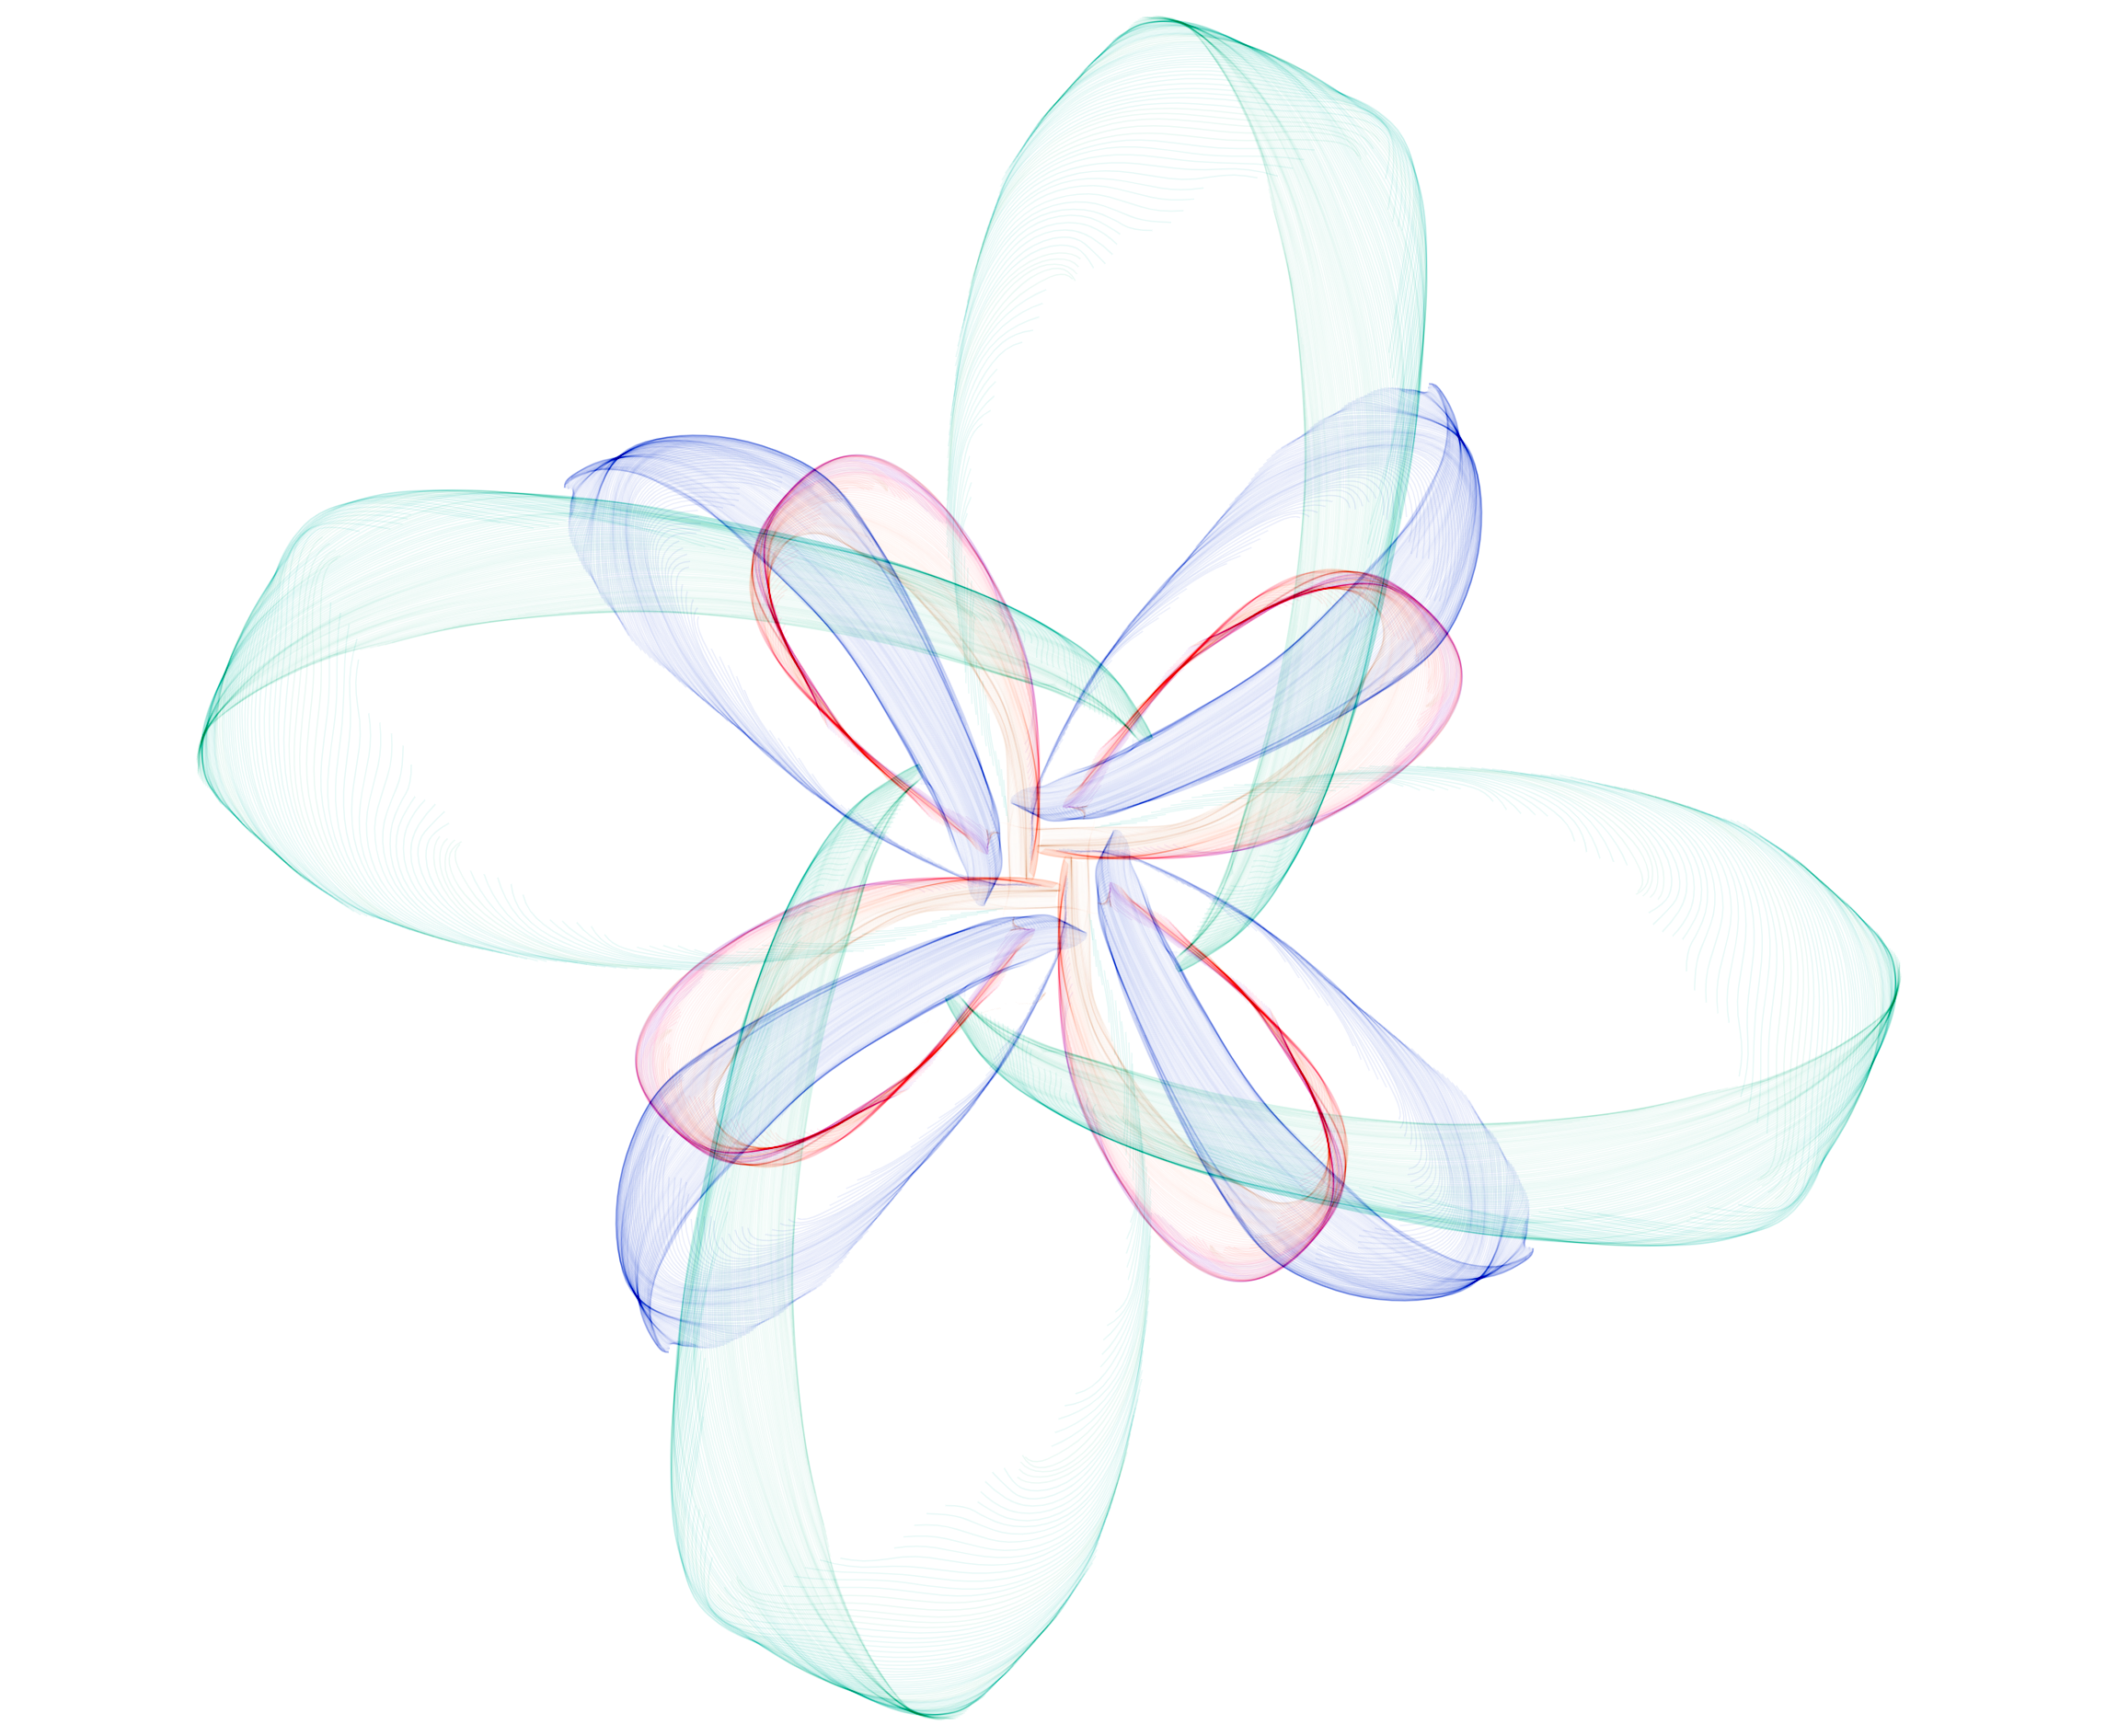
\includegraphics[width=15.5cm]{picture/cover6.png}
	%\includegraphics[width=8cm]{cover2.png}
	%\includegraphics[width=8cm]{cover3.png}
	%\includegraphics[width=12cm]{cover4.png}
\end{center}
}
		\author{
		{\CJKfamily{kai} \large {易鹏}}\\
		{\CJKfamily{kai} \large 中山大学}\vspace*{0.5em}\\
		内部版本号:V4.62.84(正式版)
}


%调整间距(倍数)
\linespread{1.5}

%自定义页眉页脚---------------
\pagestyle{fancy}
\renewcommand{\chaptermark}[1]{\markboth{\;第\ \thechapter\ 章\quad#1\;}{}}
\renewcommand{\sectionmark}[1]{\markright{\;\thesection\ #1\;}}
\fancyhf{}
%\fancyfoot[C]{\bfseries\thepage}
\fancyhead[LO]{\small\CJKfamily{song}\rightmark}
\fancyhead[RE]{\small\CJKfamily{song}\leftmark}
\fancyhead[RO,LE]{\;\thepage\;}
\fancyfoot[RO,LE]{\footnotesize\CJKfamily{heilight}{空间解析几何}}
\fancyfoot[RE,LO]{\footnotesize\CJKfamily{heilight}Analytic Geometry of Space}
\renewcommand{\headrulewidth}{0.4pt} % 注意不用\setlength
%\renewcommand{\footrulewidth}{0pt}
\fancyheadoffset[LE,RO]{0cm}
\fancyfootoffset[LE,RO]{0cm}
% 注意不用\setlength
%\renewcommand{\footrulewidth}{0pt}

%自定义命令
\newcommand{\link}[1][]{\hyperref[#1] {\color{超链接}#1}}%超链接简化命令
\newcommand{\sj}{\vspace*{-1em}}
\newcommand{\sja}{\vspace*{-0.5em}}
\newcommand{\jg}{\vspace*{1em}}
\newcommand{\eqkg}{$\,$}
\newcommand{\kg}{\hspace*{1em}}
\newcommand{\huo}{\mbox{或}}


%文档开始
\begin{document}

%标题及目录
\pagenumbering{Roman}
\clearpage {\pagestyle{empty}}
\maketitle
\setcounter{page}{1}
\tableofcontents

%正文部分
\newpage
\setcounter{page}{1}
\pagenumbering{arabic}


%第一章

\chapter{向量代数}
\section{向量的基本概念}
\subsection{几何概念}
\thispagestyle{empty}
\vspace*{-0.5cm}
\enupdefination[向量相关几何概念]
\begin{enumerate}[]
	\setlength{\itemindent}{3em}
	\setlength{\topsep}{0.01em}
	\setlength{\itemsep}{0.01em}
	\item \quad 
	\begin{figure}[h]
		\centering
		\begin{minipage}{0.8\linewidth}
			\item $\bullet$\quad {\color{dy2}向量\index{XL@向量!XL@向量}}:既有大小又有方向的量. 用符号\boldmath$a,b,c,\cdots ,$\unboldmath 或$\overrightarrow{a},\overrightarrow b$,\\$\overrightarrow{c},\cdots $表示.
			\item $\bullet$\quad {\color{dy2}向量的模\index{XL@向量!XLDM@向量的模}}:一个向量$\overrightarrow{a}$可以用一条有向线段$\overrightarrow{AB}$来表示,那么线段的长度$|AB|$就叫做向量的模(长度).用起点$A$到终点$B$的指向来表示向量量$\overrightarrow{a}$的方向.如图\ref{向量}. 
			\item $\bullet$\quad {\color{dy2}零向量\index{XL@向量!LXL@零向量}}:长度为$0$的向量. 记作$0$. {\color{dy}零向量的方向不确定. }
			\item $\bullet$\quad {\color{dy2}单位向量\index{XL@向量!DWXL@单位向量}}:长度为$1$的向量. 与$\overrightarrow{a}$同向的单位向量记作$\overrightarrow{a^0}$
			\item $\bullet$\quad {\color{dy2}反向量\index{XL@向量!FXL@反向量}}:与原向量大小相等方向相反的向量. 记作$-\overrightarrow{a}$.
		\end{minipage}%
		\hfill
		\begin{minipage}{0.2\linewidth}
			\centering
			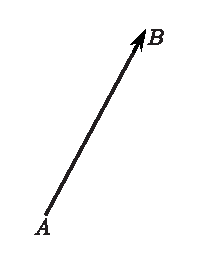
\includegraphics[width=0.9\linewidth]{picture/C-1/1.1/xl1}
			\caption{向量的表示}
			\label{向量}
		\end{minipage}%
	\end{figure}
\end{enumerate}

\subsection{解析概念}
\vspace*{-0.5cm}
\enupdefination[向量解析相关概念]
\begin{enumerate}[]
	\setlength{\itemindent}{3em}
	\setlength{\topsep}{0.01em}
	\setlength{\itemsep}{0.01em}
	\item 
	\item $\bullet$\quad{\color{dy2}基\index{XL@向量!J@基}}:空间中任意三个有次序的不共面的向量$\overrightarrow{e_1},\overrightarrow{e_2},\overrightarrow{e_3}$称为空间中的一组基.
	\item $\bullet$\quad{\color{dy2}坐标\index{XL@向量!ZB@坐标}}:对于空间中任一向量$\overrightarrow m$,若
	\begin{equation}
		\overrightarrow{m}=x\overrightarrow{e_1}+y\overrightarrow{e_2}+z\overrightarrow{e_3}
	\end{equation}
	则把有序三元实数组$(x,y,z)$称为$\overrightarrow{m}$在基$\overrightarrow{e_1},\overrightarrow{e_2},\overrightarrow{e_3}$中的坐标.
	\item $\bullet$\quad{\color{dy2}定位向量(矢径)\index{XL@向量!DWXL@定位向量}}:在空间中取定一个点$O$以后,任意一个点$M$与向量$\overrightarrow{OM}$一一对应,因此称$\overrightarrow{OM}$为点$M$的定位向量(矢径\index{XL@向量!SJ@矢径}). 
\end{enumerate}

	\begin{figure}[h]
		\sj 
\defination[坐标系相关概念]
\end{figure}

\begin{enumerate}[]
	\setlength{\itemindent}{3em}
	\setlength{\topsep}{0.01em}
	\setlength{\itemsep}{0.01em}
	\begin{figure}[h]
		\begin{minipage}{0.6\linewidth}
			\item $\bullet$\quad{\color{dy2}仿射坐标系}\index{FSZBX@仿射坐标系!FSZBX@仿射坐标系}:空间中的一个点$O$和一组基$\overrightarrow{e_1},\overrightarrow{e_2},\overrightarrow{e_3}$合在一起称为空间的一个{\color{dy2}仿射标架}或{\color{dy2}仿射坐标系}\index{FSZBX@仿射坐标系!FSBJ@仿射标架},记作$[O;\overrightarrow{e_1},\overrightarrow{e_2},\overrightarrow{e_3}]$,其中$O$称为{\color{dy2}原点}\index{FSZBX@仿射坐标系!YD@原点}. {\color{dy}特别地,当仿射坐标系的基向量两两垂直时,称为直角坐标系\index{FSZBX@仿射坐标系!ZJZBX@直角坐标系}}.
			\item $\bullet$\quad{\color{dy2}坐标轴\index{FSZBX@仿射坐标系!ZBJ@坐标轴}}:过原点$O$,且分别以$\overrightarrow{e_1},\overrightarrow{e_2},\overrightarrow{e_3}$为方向得有向直线分别称为$x$轴,$y$轴,$z$轴,统称为{\color{dy2}坐标轴}. 
			\item$\bullet$\quad {\color{dy2}坐标平面\index{FSZBX@仿射坐标系!ZBPM@坐标平面}}:由每两根坐标轴决定的平面称为{\color{dy2}坐标平面},分别为$xOy,yOz,zOx$平面. 
			\item $\bullet$\quad{\color{dy2}卦限\index{FSZBX@仿射坐标系!GX@卦限}}:坐标平面把空间分成八个部分,称为八个{\color{dy2}卦限}. 如图\ref{八卦}. 
			\item $\bullet$\quad{\color{dy2}左右手系}:将右手的拇指和食指分别指着$x$轴,$y$轴,如果中值所指的方向与$z$轴方向在$xOy$平面同侧,则称此坐标系为{\color{dy2}右手系\index{FSZBX@仿射坐标系!YSX@右手系}},否则称为{\color{dy2}左手系\index{FSZBX@仿射坐标系!ZSX@左手系}}. 
		\end{minipage}
		\hfill
		\begin{minipage}{0.4\linewidth}
			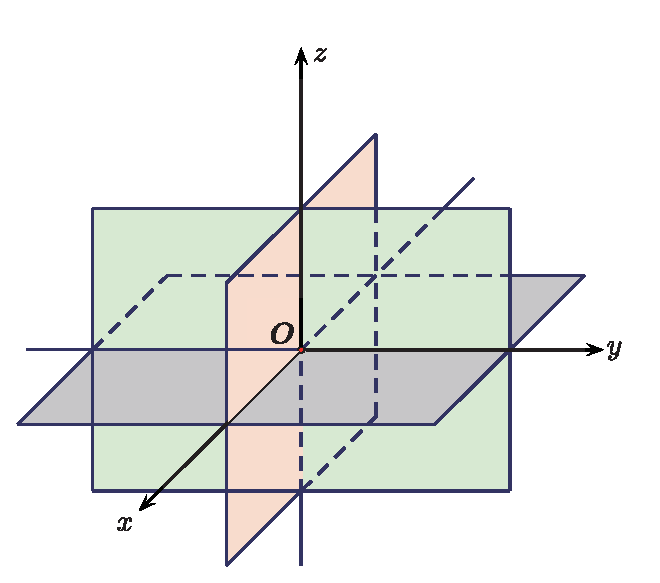
\includegraphics[scale=0.75]{picture/C-1/1.1/BG.eps}
			\caption{仿射坐标系及其八卦}
			\label{八卦}
		\end{minipage}
	\end{figure}
\end{enumerate}
\jg
\jg

\subsection{方向角与方向余弦}
\tdefination[向量的夹角]\index{XL@向量!XLDJJ@向量的夹角}
设有两个非零向量$\overrightarrow{a}$,$\overrightarrow{b}$,任取空间中一点$O$ ,作$\overrightarrow{OA}=\overrightarrow{a},\overrightarrow{OB}=\overrightarrow{b}$,规定$0\le \varphi=\angle AOB\le \pi $,那么$\angle AOB$称为向量$\overrightarrow{a}$,$\overrightarrow{b}$的夹角,即$0\le\left\langle \overrightarrow{a},\overrightarrow{b}\right\rangle =\left\langle \overrightarrow{b},\overrightarrow{a}\right\rangle =\varphi\le \pi $.

\begin{figure}[h]
	\begin{minipage}{0.5\linewidth}
		\centering 
		\includegraphics[width=0.9\linewidth]{picture/C-1/1.1/angle.eps}
		\caption{向量的夹角}
	\end{minipage}
	\hfill
	\begin{minipage}{0.5\linewidth}
		\centering 
		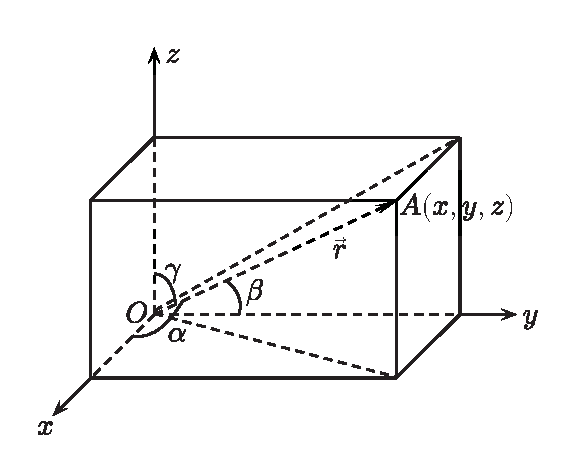
\includegraphics[width=0.9\linewidth]{picture/C-1/1.1/angle2.eps}
		\caption{方向角与方向余弦}
	\end{minipage}
\end{figure}
\newpage 
\defination[方向角与方向余弦]\index{FSZBX@仿射坐标系!FXJYFXYX@方向角与方向余弦}
\quad 记非零向量$\overrightarrow{r}$与三条坐标轴($x$轴,$y$轴,$z$轴)的夹角分别为$\alpha ,\beta ,\gamma$.称为向量$\overrightarrow{r}$的方向角.设$\overrightarrow{r}=\overrightarrow{OA}=(x,y,z)$,若$\sqrt{x^2+y^2+z^2}\ne 0,$则
\begin{equation*}
	\cos \alpha =\frac{x}{|\overrightarrow{r}|}=\frac{x}{	\sqrt{x^2+y^2+z^2}}\qquad 
	\cos \beta =\frac{y}{|\overrightarrow{r}|}=\frac{y}{	\sqrt{x^2+y^2+z^2}}\qquad
	\cos \gamma =\frac{z}{|\overrightarrow{r}|}=\frac{z}{	\sqrt{x^2+y^2+z^2}}
\end{equation*}

\section{向量的基本运算}
\subsection{线性运算}\index{XXYS@线性运算!XXYS@线性运算}
\begin{enumerate}
	\setlength{\itemindent}{0em}
	\setlength{\topsep}{0.01em}
	\setlength{\itemsep}{0.01em}
	\item {\color{dy}加(减)法\index{XXYS@线性运算!JF@加法}}
	\begin{enumerate}[(1)]
		\setlength{\topsep}{0.01em}
		\setlength{\itemsep}{0.01em}
		\item {\color{dy2}几何表示}
		\begin{enumerate}[]
					\setlength{\itemindent}{1em} 
			\setlength{\topsep}{0.01em}
			\setlength{\itemsep}{0.01em}
			\item 对于向量 $\overrightarrow a,\overrightarrow b$,作有向线段 ,作有向线段 $\overrightarrow {AB}$表示 $\overrightarrow a$,作 $\overrightarrow {BC}$表示 $\overrightarrow b$,则把有向线段 $\overrightarrow {AC}$表示的向量 $\overrightarrow c$称为 向量$\overrightarrow a$与$\overrightarrow b$的和 .向量加法运算规则在几何上称为向量加法运算规则在几何上称为{\color{dy}三角形法则\index{XXYS@线性运算!JF@加法!SJXFZ@三角形法则}}或{\color{dy}平行四边形法则\index{XXYS@线性运算!JF@加法!PXSBXFZ@平行四边形法则}} .如图\ref{向量加法}.
			\begin{figure}[h]
				\centering
				\subfigure[三角形法则]{
					\begin{minipage}[t]{0.5\linewidth}
						\centering
						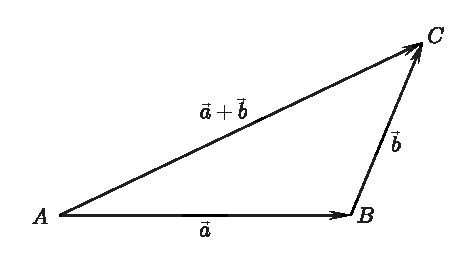
\includegraphics[width=0.9\linewidth]{picture/C-1/1.2/JF2}
						%\caption{fig1}
					\end{minipage}%
				}%
				\subfigure[平行四边形法则]{
					\begin{minipage}[t]{0.5\linewidth}
						\centering
						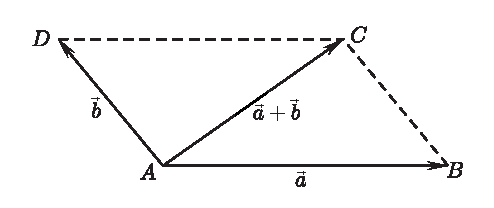
\includegraphics[width=0.9\linewidth]{picture/C-1/1.2/JF1}
						%\caption{fig2}
					\end{minipage}%
				}%
				
				\centering
				\caption{向量的加法法则}
				\label{向量加法}
			\end{figure}
		\end{enumerate}
		\item {\color{dy2}坐标表示}
		\begin{enumerate}[]
					\setlength{\itemindent}{1em} 
			\setlength{\topsep}{0.01em}
			\setlength{\itemsep}{0.01em}
			\item 设$\overrightarrow a = (x_1,y_1,z_1),\overrightarrow b = (x_2,y_2,z_2)$,则$\overrightarrow a +\overrightarrow b =(x_1+x_2,y_1+y_2,z_1+z_2)$
		\end{enumerate}
		\item {\color{dy2}运算律}
		\begin{enumerate}
					\setlength{\itemindent}{1em} 
			\setlength{\topsep}{0.01em}
			\setlength{\itemsep}{0.01em}
			\begin{minipage}{0.6\linewidth}
				\item 交换律:$\overrightarrow a+\overrightarrow b =\overrightarrow b+\overrightarrow a$
				\item 结合律:$\left( \overrightarrow a+\overrightarrow b\right)  +\overrightarrow  c= \overrightarrow a+\left( \overrightarrow b  +\overrightarrow  c\right) $
				\item 任意向量$\overrightarrow{a}$,有$\overrightarrow{a}+\overrightarrow{0}$
				\item 任意向量$\overrightarrow{a}$,有$\overrightarrow{a}-\overrightarrow{a}=\overrightarrow{0}$
				\item 向量的减法:$\overrightarrow{a} - \overrightarrow{b} =\overrightarrow{a} +(- \overrightarrow{b} )$
			\end{minipage}
			\hfill
			\begin{minipage}{0.4\linewidth}
				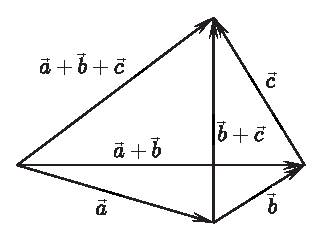
\includegraphics[width=0.9\linewidth]{picture/C-1/1.2/JF3}
			\end{minipage}
		\end{enumerate}
	\end{enumerate}
\newpage
	\item {\color{dy}数乘\index{XXYS@线性运算!SC@数乘}}
	\begin{enumerate}[(1)]
		\setlength{\topsep}{0.01em}
		\setlength{\itemsep}{0.01em}
		\item{\color{dy2}几何表示}
		\begin{enumerate}
			实数$\lambda$与向量$\overrightarrow a$的乘积定义为一个向量$\lambda \overrightarrow{a}$它的长度为
			\begin{equation}
				\left| \lambda \overrightarrow{a}\right| =|\lambda |\cdot \left| \overrightarrow{a}\right|
			\end{equation} 
			当 $\lambda >0$时它的方向与 $\overrightarrow{a}$相同,当 $\lambda <0$时它的方向与 $\overrightarrow{a}$相反 .
		\end{enumerate}
		\item {\color{dy2}坐标表示}
		\begin{enumerate}[]
					\setlength{\itemindent}{1em} 
			\setlength{\topsep}{0.01em}
			\setlength{\itemsep}{0.01em}
			\item 设$\overrightarrow a = (x,y,z)$,则$\lambda\overrightarrow{a}=(\lambda x,\lambda y,\lambda z)$
		\end{enumerate}
		\item{\color{dy2} 运算律}
		\begin{enumerate}
					\setlength{\itemindent}{1em} 
			\setlength{\topsep}{0.01em}
			\setlength{\itemsep}{0.01em}
			\item 结合律:$\lambda (\mu \overrightarrow{a})=(\lambda \mu )\overrightarrow{a}$
			\item 分配律:$(\lambda + \mu )\overrightarrow{a}=\lambda \overrightarrow{a}+\mu \overrightarrow{a} , \qquad \lambda(\overrightarrow{a}+\overrightarrow{b})=\lambda \overrightarrow{a}+\lambda \overrightarrow{b}.$
		\end{enumerate}
	\end{enumerate}
\end{enumerate}
\subsection{线性组合}
\tdefination[线性组合]\index{XXXGX@线性相关性!XXZH@线性组合}
一般地,设 $\overrightarrow {a_1},\overrightarrow {a_2},\cdots ,\overrightarrow {a_m}$是一组向量, $k_1,k_2,\cdots ,k_m$是一组实数,称向量 $k_1\overrightarrow{ a_1},k_2\overrightarrow {a_2},\cdots ,k_m\overrightarrow{ a_m}$为该向量组的一个 {\color{dy}线性组合},称$k_1,k_2,\cdots ,k_m$为这个 {\color{dy}线性组合的系数\index{XXXGX@线性相关性!XXZHDXS@线性组合的系数}}. 


\adddefination[线性相关性]\index{XXXGX@线性相关性!XXXGX@线性相关性}
一般地,设 $\overrightarrow {a_1},\overrightarrow {a_2},\cdots ,\overrightarrow {a_m}$是一组向量,如果存在 一组不全为零的实数$k_1,k_2,\cdots ,k_m$使得:
\begin{equation}
	k_1\overrightarrow{a_1}+k_2\overrightarrow{a_2}+\cdots +k_m\overrightarrow{a_m}=0
	\label{线性相关}
\end{equation}
那么称向量$\overrightarrow {a_1},\overrightarrow {a_2},\cdots ,\overrightarrow {a_m}$ {\color{dy}线性相关}\index{XXXGX@线性相关性!XXXG@线性相关}. 否则称向量组为{\color{dy}线性无关\index{XXXGX@线性相关性!XXWG@线性无关}}.\\
\quad 向量线性相关性的几何意义:线性相关性与向量是否在同一个向量空间等价. 在二阶和三阶向量空间中,向量是否线性相关代表着向量是否共线或共面. 
\jg
\jg
\subsection{内积}\index{NJ@内积}
\begin{enumerate}[1.]
			\setlength{\itemindent}{0em} 
	\setlength{\topsep}{0.01em}
	\setlength{\itemsep}{0.01em}
	\item {\color{dy2}几何表示}
	\begin{enumerate}[]
				\setlength{\itemindent}{1.5em} 
		\setlength{\topsep}{0.01em}
		\setlength{\itemsep}{0.01em}
		\item \begin{equation}
			\overrightarrow{a} \cdot \overrightarrow{b}=|\overrightarrow{a}|\cdot |\overrightarrow{b}| \cos \left\langle \overrightarrow{a},\overrightarrow{b}	\right\rangle 
		\end{equation}
	\end{enumerate}
	\newpage
	\item {\color{dy2}坐标表示}
	\begin{enumerate}[]
				\setlength{\itemindent}{1.5em} 
		\setlength{\topsep}{0.01em}
		\setlength{\itemsep}{0.01em}
		\item 设在仿射标架$[O,\overrightarrow{e_1},\overrightarrow{e_2},\overrightarrow{e_3}]$中$\overrightarrow{a},\overrightarrow{b}$的坐标分别为:$(a_1,a_2,a_3),(b_1,b_2,b_3)$,则
		\begin{equation}
			\begin{aligned}
				\overrightarrow{a} \cdot   \overrightarrow{b}&=(a_1\overrightarrow{e_1}+a_2\overrightarrow{e_2}+a_3\overrightarrow{e_3})\cdot   (b_1\overrightarrow{e_1}+b_2\overrightarrow{e_2}+b_3\overrightarrow{e_3})\\
				&=a_1b_1\cdot  \left[\overrightarrow{e_1}\cdot   \overrightarrow{e_1}\right]+a_1b_2\cdot  \left[\overrightarrow{e_1}\cdot   \overrightarrow{e_2}\right]+a_1b_3\cdot  \left[\overrightarrow{e_1}\cdot  \overrightarrow{e_3}\right]\\
				&\,\,+a_2b_1\cdot  \left[\overrightarrow{e_2}\cdot   \overrightarrow{e_1}\right]+a_2b_2\cdot  \left[\overrightarrow{e_2}\cdot   \overrightarrow{e_2}\right]+a_2b_3\cdot  \left[\overrightarrow{e_2}\cdot  \overrightarrow{e_3}\right]\\
				&\,\,+a_3b_1\cdot  \left[\overrightarrow{e_3}\cdot   \overrightarrow{e_1}\right]+a_3b_2\cdot  \left[\overrightarrow{e_3}\cdot   \overrightarrow{e_2}\right]+a_3b_3\cdot  \left[\overrightarrow{e_3}\cdot   \overrightarrow{e_3}\right]
			\end{aligned}
		\end{equation}
		\qquad 因此,我们要知道两个向量的内积,只需要知道向量$\overrightarrow{e_1},\overrightarrow{e_2},\overrightarrow{e_3}$的内积(九个数)即可,这九个数称为{\color{dy}仿射标架$[O,\overrightarrow{e_1},\overrightarrow{e_2},\overrightarrow{e_3}]$的度量参数\index{FSZBX@仿射坐标系!DLCS@度量参数}}. \\
		\hspace*{2em}特别地,当仿射坐标系的基向量两两垂直时,即为直角坐标系时,内积表达式可写为
		\begin{equation}
			\overrightarrow{a} \cdot \overrightarrow{b}=a_1b_1+a_2b_2+a_3b_3.
		\end{equation}
	\end{enumerate}
	\item {\color{dy2}运算律}
	\begin{enumerate}[i.]
				\setlength{\itemindent}{1.5em} 
		\setlength{\topsep}{0.01em}
		\setlength{\itemsep}{0.01em}
		\item 对称性:$\overrightarrow{a}\cdot \overrightarrow{b}=\overrightarrow{b}\cdot \overrightarrow{a}.$
		\item 数线性:$(\lambda\overrightarrow{a})\cdot \overrightarrow{b}=\overrightarrow{a}\cdot (\lambda \overrightarrow{b}).$
		\item 向量线性:$(\overrightarrow{a}+\overrightarrow{b})\cdot \overrightarrow{c}=\overrightarrow{a}\cdot \overrightarrow{c}+\overrightarrow{b}\cdot\overrightarrow{c}.$
	\end{enumerate}
\end{enumerate}
\jg
\jg
\subsection{外积}\index{WJ@外积}
\begin{enumerate}[1.]
			\setlength{\itemindent}{0em} 
	\setlength{\topsep}{0.01em}
	\setlength{\itemsep}{0.01em}
	\item {\color{dy2}几何表示}\vspace{0.25cm}
	\begin{enumerate}[]
				\setlength{\itemindent}{1.5em} 
		\setlength{\topsep}{0.01em}
		\setlength{\itemsep}{0.01em}
		\begin{figure}[htb]
			\begin{minipage}{0.6\linewidth}
				\item 两个向量$\overrightarrow{a},\overrightarrow{b}$的外积仍然是一个向量,它的长度为
				\begin{equation}
					\left|\overrightarrow{a}\times\overrightarrow{b} \right| =|\overrightarrow{a}|\cdot |\overrightarrow{b}|\sin \left\langle \overrightarrow{a},\overrightarrow{b}\right\rangle 
				\end{equation}
				\item 它的方向为与$\overrightarrow{a},\overrightarrow{b}$构成的平面垂直,右手螺旋为逆时针,则垂直该平面向上;右手螺旋为顺时针,则垂直该平面向下. 
				\item {\color{dy}几何意义}\label{外积的几何意义} :$\left|\overrightarrow{a}\times\overrightarrow{b} \right|$代表的是分别以$\overrightarrow{a},\overrightarrow{b}$为邻边的平行四边形的面积. 如图\ref{外积}.
			\end{minipage}
			\hfill
			\begin{minipage}{0.4\linewidth}
				\centering
				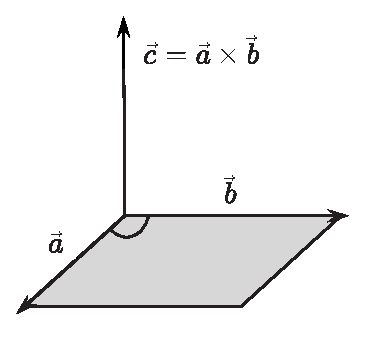
\includegraphics[width=0.7\linewidth]{picture/C-1/1.2/WJ.eps}
				\caption{外积的几何意义}
				\label{外积}
			\end{minipage}
		\end{figure}
	\end{enumerate}
	\newpage
	\item {\color{dy2}坐标表示}
	\begin{enumerate}[]
				\setlength{\itemindent}{1.5em} 
		\setlength{\topsep}{0.01em}
		\setlength{\itemsep}{0.01em}
		\item 设在仿射标架$[O,\overrightarrow{e_1},\overrightarrow{e_2},\overrightarrow{e_3}]$中$\overrightarrow{a},\overrightarrow{b}$的坐标分别为:$(a_1,a_2,a_3),(b_1,b_2,b_3)$,则
		\begin{equation}
			\begin{aligned}
				\overrightarrow{a} \times \overrightarrow{b}&=(a_1\overrightarrow{e_1}+a_2\overrightarrow{e_2}+a_3\overrightarrow{e_3})\times (b_1\overrightarrow{e_1}+b_2\overrightarrow{e_2}+b_3\overrightarrow{e_3})\\
				&=a_1b_1\cdot  \left[\overrightarrow{e_1}\times \overrightarrow{e_1}\right]+a_1b_2\cdot  \left[\overrightarrow{e_1}\times \overrightarrow{e_2}\right]+a_1b_3\cdot  \left[\overrightarrow{e_1}\times\overrightarrow{e_3}\right]\\
				&\,\, +a_2b_1\cdot  \left[\overrightarrow{e_2}\times \overrightarrow{e_1}\right]+a_2b_2\cdot  \left[\overrightarrow{e_2}\times \overrightarrow{e_2}\right]+a_2b_3\cdot  \left[\overrightarrow{e_2}\times\overrightarrow{e_3}\right]\\
				&\,\,  +a_3b_1\cdot  \left[\overrightarrow{e_3}\times \overrightarrow{e_1}\right]+a_3b_2\cdot  \left[\overrightarrow{e_3}\times \overrightarrow{e_2}\right]+a_3b_3\cdot  \left[\overrightarrow{e_3}\times \overrightarrow{e_3}\right]\\
				&=\left( a_1b_2-a_2b_1\right)\cdot \left[\overrightarrow{e_1}\times \overrightarrow{e_2}\right]+\left(a_3b_1-a_1b_3\right)\cdot \left[\overrightarrow{e_3}\times \overrightarrow{e_1}\right]+\left(a_2b_3-a_3b_2\right)\cdot \left[\overrightarrow{e_2}\times \overrightarrow{e_3}\right] \\
				&=\begin{array}{|ccc|}
					\left[\overrightarrow{e_1}\times \overrightarrow{e_2}\right]&\left[\overrightarrow{e_3}\times \overrightarrow{e_1}\right]  &\left[\overrightarrow{e_2}\times \overrightarrow{e_3}\right]  \\
					a_1 & a_2 & a_3 \\
					b_1 & b_2 & b_3
				\end{array}
			\end{aligned}
		\end{equation}
		\qquad 因此,我们要知道任意两个向量的外积,只需要知道向量$\overrightarrow{e_1},\overrightarrow{e_2},\overrightarrow{e_3}$的外积(三个向量)即可. \\
		\hspace*{2em}特别地,当仿射坐标系的基向量两两垂直时,即为直角坐标系时,外积表达式可写为:
		\begin{equation}
			\overrightarrow{a} \times \overrightarrow{b}=\left( a_2b_3-a_3b_2\right)\cdot \overrightarrow{e_1}+\left(a_3b_1-a_1b_3\right)\cdot  \overrightarrow{e_2}+\left(a_1b_2-a_2b_1\right)\cdot \overrightarrow{e_3} =\begin{array}{|ccc|}
				\overrightarrow{e_1}& \overrightarrow{e_2} & \overrightarrow{e_3} \\
				a_1 & a_2 & a_3 \\
				b_1 & b_2 & b_3
			\end{array}
		\end{equation}
	\end{enumerate}
			\item  {\color{dy2}运算律}
	\begin{figure}[h]
		\begin{minipage}{0.5\linewidth}
			\begin{enumerate}[i]
						\setlength{\itemindent}{1.5em} 
				\setlength{\topsep}{0.01em}
				\setlength{\itemsep}{0.01em}
				\item 反交换律:$\overrightarrow{a}\times \overrightarrow{b}=-\overrightarrow{b}\times \overrightarrow{a}$
				\item 数乘线性:$(\lambda \overrightarrow{a})\times \overrightarrow{b}=\lambda (\overrightarrow{a}\times \overrightarrow{b})$
				\item 左分配律:$\overrightarrow{a}\times (\overrightarrow{b}+\overrightarrow{c})=\overrightarrow{a}\times \overrightarrow{b}+\overrightarrow{a}\times \overrightarrow{c}$
				\item 右分配律:$(\overrightarrow{b}+\overrightarrow{c})\times \overrightarrow{a}=\overrightarrow{b}\times \overrightarrow{a}+ \overrightarrow{c}\times \overrightarrow{a} $
			\end{enumerate}
		\end{minipage}
		\hfill
		\begin{minipage}{0.4\linewidth}
			\centering
			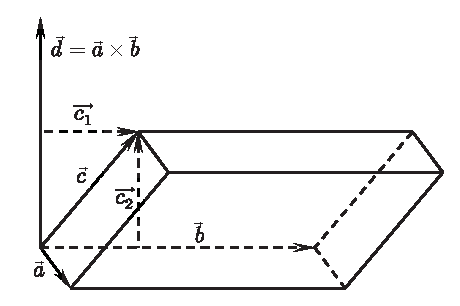
\includegraphics[width=0.9\linewidth]{picture/C-1/1.2/HHJ.eps}
			\caption{外积的几何意义}
			\label{混合积}
		\end{minipage}
	\end{figure}
\end{enumerate}
\subsection{混合积}\index{HHJ@混合积}
\begin{enumerate}[1.]
			\setlength{\itemindent}{1.5em} 
	\setlength{\topsep}{0.01em}
	\setlength{\itemsep}{0.01em}
	\item {\color{dy2}几何表示}
	\begin{enumerate}[]
				\setlength{\itemindent}{1.5em} 
		\setlength{\topsep}{0.01em}
		\setlength{\itemsep}{0.01em}
		\item 两个向量$\overrightarrow{a},\overrightarrow{b}$的外积后与另一个向量$\overrightarrow{c}$内积后是一个数,记为
		\begin{equation}
			\left( \overrightarrow{a}\times\overrightarrow{b}\right) \cdot \overrightarrow{c}
		\end{equation}
		\item {\color{dy}几何意义}\label{混合积的几何意义}:$\left|\overrightarrow{a}\times\overrightarrow{b}\cdot \overrightarrow{c} \right|$代表的是分别以$\overrightarrow{a},\overrightarrow{b},\overrightarrow{c}$为邻边的平行六面体的体积. 如图\ref{混合积}.
	\end{enumerate}

	\item {\color{dy2}坐标表示}
	\begin{enumerate}[]
				\setlength{\itemindent}{1.5em} 
		\setlength{\topsep}{0.01em}
		\setlength{\itemsep}{0.01em}
		\item 设在仿射标架$[O,\overrightarrow{e_1},\overrightarrow{e_2},\overrightarrow{e_3}]$中$\overrightarrow{a},\overrightarrow{b},\overrightarrow{c}$的坐标分别为:$(a_1,a_2,a_3),(b_1,b_2,b_3),(c_1,c_2,c_3)$,则
		\begin{equation}
			\begin{aligned}
				(\overrightarrow{a} \times \overrightarrow{b})\cdot \overrightarrow{c}&=(a_1\overrightarrow{e_1}+a_2\overrightarrow{e_2}+a_3\overrightarrow{e_3})\times (b_1\overrightarrow{e_1}+b_2\overrightarrow{e_2}+b_3\overrightarrow{e_3})\\
				&=\left( a_1b_2-a_2b_1\right)\cdot \left[\overrightarrow{e_1}\times \overrightarrow{e_2}\right]+\left(a_3b_1-a_1b_3\right)\cdot \left[\overrightarrow{e_3}\times \overrightarrow{e_1}\right]\\
				&\quad +\left(a_2b_3-a_3b_2\right)\cdot \left[\overrightarrow{e_2}\times \overrightarrow{e_3}\right]\cdot \left( c_1\overrightarrow{e_1}+c_2\overrightarrow{e_2}+c_3\overrightarrow{e_3}\right) \\
				&=[(a_1b_2-a_2b_1)c_3+(a_3b_1-a_1b_3)c_2+(a_2b_3-a_3b_2)c_1]\,\,(\overrightarrow{e_1}\times \overrightarrow{e_2}\cdot \overrightarrow{e_3})\\
				&=\begin{array}{|ccc|}
					a_1 & a_2 & a_3 \\
					b_1 & b_2 & b_3 \\
					c_1 & c_2 & c_3
				\end{array}\cdot (\overrightarrow{e_1}\times \overrightarrow{e_2}\cdot \overrightarrow{e_3})
			\end{aligned}
		\end{equation}
		\addentheorem[混合积表示]{设在仿射标架$[O,\overrightarrow{e_1},\overrightarrow{e_2},\overrightarrow{e_3}]$中$\overrightarrow{a},\overrightarrow{b},\overrightarrow{c}$的坐标分别为:$(a_1,a_2,a_3)$,\\
			$(b_1,b_2,b_3),(c_1,c_2,c_3)$,则
			\begin{equation}
				\frac{(\overrightarrow{a} \times \overrightarrow{b})\cdot \overrightarrow{c}}{(\overrightarrow{e_1}\times \overrightarrow{e_2})\cdot \overrightarrow{e_3}}=
				\begin{array}{|ccc|}
					a_1 & a_2 & a_3 \\
					b_1 & b_2 & b_3 \\
					c_1 & c_2 & c_3
				\end{array}
			\end{equation}
			特别地,当仿射坐标系的基向量两两垂直时,即为直角坐标系时,混合积表达式可写为:
			\begin{equation}
				(\overrightarrow{a} \times \overrightarrow{b})\cdot \overrightarrow{c}=
				\begin{array}{|ccc|}
					a_1 & a_2 & a_3 \\
					b_1 & b_2 & b_3 \\
					c_1 & c_2 & c_3
				\end{array}
			\end{equation}
		}
	\end{enumerate}
	\item {\color{dy2}性质}
	\begin{equation}
		\left( \overrightarrow{a}\times \overrightarrow{b}\right) \cdot \overrightarrow{c}=\left( \overrightarrow{b}\times \overrightarrow{c}\right) \cdot \overrightarrow{a}=\left( \overrightarrow{c}\times\overrightarrow{a}\right) \cdot \overrightarrow{b}=\overrightarrow{a}\cdot \left( \overrightarrow{b}\times \overrightarrow{c}\right) .
	\end{equation}
	即混合积的轮换式相等$(a,b,c)=(b,c,a)=(c,a,b)$,任意两个向量交换顺序都要加上负号. \\
\end{enumerate}
\subsection{射影和分量}
\tdefination[射影]
\hspace*{0.3cm} 若向量$\overrightarrow{a}=\overrightarrow{ a_1}+\overrightarrow{a_2}$,其中$\overrightarrow{a_1}\parallel \overrightarrow{e},\overrightarrow{ a_2}\perp \overrightarrow{e},\overrightarrow{e}$是单位向量,则称$\overrightarrow{a_1}$是在$\overrightarrow{e}$方向上的{\color{dy}内射影\index{SY@射影!NSY@内射影}(简称射影\index{SY@射影!SY@射影})},也称{\color{dy}投影向量\index{SY@射影!TYXL@投影向量}};称$\overrightarrow{a_1}$是在$\overrightarrow{e}$方向$\overrightarrow{e}$下的{\color{dy}外射影\index{SY@射影!WSY@外射影}}.

\begin{figure}[h]
	\begin{minipage}{0.65\linewidth}
		\defination[分量]
		\hspace*{0.3cm} 若向量$\overrightarrow{a_1}$是$\overrightarrow{a}$在方向$\overrightarrow{e}$(单位向量)上的内射影,则存在唯一的实数$\lambda $使得$\overrightarrow{a_1}=\lambda \overrightarrow{e}$,这个实数$\lambda $被称为$\overrightarrow{a}$在方向$\overrightarrow{e}$上的{\color{dy}分量\index{SY@射影!FL@分量}(也称投影\index{SY@射影!TY@投影})},记作$\Pi_{\overrightarrow{e}}\overrightarrow{a}$,其值为
		\begin{equation}
			\Pi_ {\overrightarrow{e}}\overrightarrow{a}=|\overrightarrow{a}|\cos \left\langle \overrightarrow{a},\overrightarrow{e}\right\rangle=\frac{\overrightarrow{a}\cdot \overrightarrow{e}}{|\overrightarrow{e}|}=\overrightarrow{a}\cdot \overrightarrow{e}.
		\end{equation}
		
	\end{minipage}
	\hfill
	\begin{minipage}{0.35\linewidth}
		\centering
		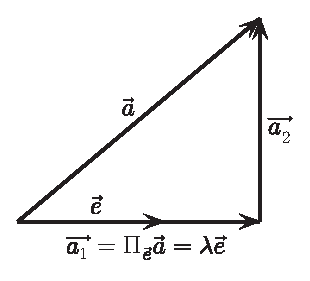
\includegraphics[width=0.7\linewidth]{picture/C-1/1.2/TY.eps}
		\caption{向量的射影}
		\label{TY}
	\end{minipage}
\end{figure}
这里特别要注意的是:射影(投影向量)是矢量,而分量(投影)才是标量!\\
\vspace*{-2em}
\subsection{二重外积}\index{ECWJ@二重外积}

\ttheorem[二重外积公式]
对任意向量$\overrightarrow{a},\overrightarrow{b},\overrightarrow{c},$有
\begin{equation}
	\overrightarrow{a}\times\left( \overrightarrow{b}\times\overrightarrow{c}\right) =\left( \overrightarrow{a}\cdot \overrightarrow{c}\right)\overrightarrow{b}-\left( \overrightarrow{a}\cdot  \overrightarrow{b}\right)\overrightarrow{c}.  
	\label{二重外积}
\end{equation}
\qquad  二重外积公式\eqref{二重外积}表明$\overrightarrow{a}\times\left( \overrightarrow{b}\times\overrightarrow{c}\right)$是向量$\overrightarrow{b},\overrightarrow{c}$的线性组合,即$\overrightarrow{a}\times\left( \overrightarrow{b}\times\overrightarrow{c}\right)$与向量$\overrightarrow{b},\overrightarrow{c}$共面. 

\section{向量共线、共面的判断条件汇总}
\subsection{向量或三点共线的通用判定条件}\index{SDGX@三点共线}
\begin{enumerate}[1.]
	\setlength{\itemindent}{0em}
	\setlength{\topsep}{0.01em}
	\setlength{\itemsep}{0.01em}
	\item {\color{dy2}几何表示}
	
	\enbelowtheorem[共线定理1]
	\quad $\overrightarrow{a},\overrightarrow{b}$共线的充分必要条件是存在不全为$0$的实数$\lambda,\mu $,使得
	\begin{equation}
		\lambda \overrightarrow{a}+\mu \overrightarrow{b}=\overrightarrow{0}
		\label{gx1}
	\end{equation}
	{\color{dy} 而$\overrightarrow{a},\overrightarrow{b}$不共线的充分必要条件是式\eqref{gx1}中$\lambda=\mu=0 $.}
	
	\addentheorem[共线定理2]
	\quad $\overrightarrow{a},\overrightarrow{b}$共线的充分必要条件是存在实数$\lambda $,使得
	\begin{equation}
		\overrightarrow{a}=\lambda \overrightarrow{b}
		\label{gx2}
	\end{equation}
	\qquad {\color{dy}注:式\eqref{gx1},\eqref{gx2}本质是线性组合和线性相关性(式\eqref{线性相关})的具体应用. }
	
	\addentheorem[共线定理3]
	\quad $\overrightarrow{a},\overrightarrow{b}$共线的充分必要条件是
	\begin{equation}
		\overrightarrow{a}\times\overrightarrow{b}=\overrightarrow{0}
	\end{equation}
	
	\item {\color{dy2}坐标表示}
	
	\enbelowtheorem[共线定理4]
	\quad 在三个点$A,B,C$所在平面上取一个仿射坐标系$[O;\overrightarrow{e_1},\overrightarrow{e_2}]$,设$A,B,C$的坐标分别是
	$$(a_1,a_2),(b_1,b_2),(c_1,c_2)$$
	则$A,B,C$三点共线的充分必要条件是
	\begin{equation}
		\begin{array}{|ccc|}
			a_1 & b_1 & c_1 \\
			a_2 & b_2 & c_2 \\
			1 & 1 & 1
		\end{array}=0
	\end{equation}
	
	\addentheorem[共线定理5]
	\quad 设仿射坐标系$[O;\overrightarrow{e_1},\overrightarrow{e_2},\overrightarrow{e_3}]$上的两个向量$\overrightarrow{a},\overrightarrow{b}$的坐标分别是$(a_1,a_2,a_3)$,\\$(b_1,b_2,b_3).$则$\overrightarrow{a},\overrightarrow{b}$共线的充分必要条件是
	\begin{equation}
		\begin{array}{|cc|}
			a_1 & b_1  \\
			a_2 & b_2 
		\end{array}=
		\begin{array}{|cc|}
			a_1 & b_1  \\
			a_3& b_3 
		\end{array}=
		\begin{array}{|cc|}
			a_2 & b_2  \\
			a_3 & b_3 
		\end{array}=0
	\end{equation}
\end{enumerate}

\subsection{向量或四点共面的通用判定条件}\index{SDGM@四点共面}
\begin{enumerate}[1.]
	\setlength{\itemindent}{0em}
	\setlength{\topsep}{0.01em}
	\setlength{\itemsep}{0.01em}
	\item {\color{dy2}几何表示}
	
	\enbelowtheorem[共面定理1]
	\quad $\overrightarrow{a},\overrightarrow{b},\overrightarrow{c}$共线的充分必要条件是存在不全为$0$的实数$k_1,k_2,k_3 $,使得
	\begin{equation}
		k_1\overrightarrow{a}+k_2\overrightarrow{b}+k_3\overrightarrow{c}=\overrightarrow{0}
		\label{gm1}
	\end{equation}
	{\color{dy} 而$\overrightarrow{a},\overrightarrow{b}$不共面的充分必要条件是式\eqref{gm1}中$k_1=k_2=k_3=0 $.}
	
	\newpage
	\addentheorem[共面定理2]
	\quad $\overrightarrow{a},\overrightarrow{b},\overrightarrow{c}$共面的充分必要条件是存在实数$\lambda ,\mu $,使得
	\begin{equation}
		\overrightarrow{c}=\lambda \overrightarrow{a}+\mu\overrightarrow{b}
		\label{gm2}
	\end{equation}
	{\color{dy}\qquad 注:式\eqref{gm1},\eqref{gm2}本质是线性组合和线性相关性(式\eqref{线性相关})的具体应用. }
	
	
	\addentheorem[共面定理3]
	\quad $\overrightarrow{a},\overrightarrow{b},\overrightarrow{c}$共面的充分必要条件是
	\begin{equation}
		\left( \overrightarrow{a}\times\overrightarrow{b}\right) \cdot \overrightarrow{c}=0
	\end{equation}
	
	\item {\color{dy2}坐标表示}
	
	\enbelowtheorem[共面定理4]
	\quad 设$\overrightarrow{a},\overrightarrow{b},\overrightarrow{c}$的仿射坐标分别为:
	$$(a_1,a_2,a_3),(b_1,b_2,b_3),(c_1,c_2,c_3)$$
	则$\overrightarrow{a},\overrightarrow{b},\overrightarrow{c}$共面的充分必要条件是
	\begin{equation}
		\begin{array}{|ccc|}
			a_1 & a_2 & a_3 \\
			b_1 & b_2 & b_3 \\
			c_1 & c_2 & c_3
		\end{array}=0
	\end{equation}
	
	
	\addentheorem[共面定理5]
	\quad 设四个点$A,B,C,D$的仿射坐标分别为:
	$$(x_1,y_1,z_1),(x_2,y_2,z_2),(x_3,y_3,z_3),(x_4,y_4,z_4)$$
	则点$A,B,C,D$共面的充分必要条件是
	\begin{equation}
		\begin{array}{|cccc|}
			x_1 & y_1 & z_1 & 1 \\
			x_2 & y_2 & z_2 & 1 \\
			x_3 & y_3 & z_3 & 1 \\
			x_4 & y_4 & z_4 & 1
		\end{array}=0
		\label{SDGM}
	\end{equation}
\end{enumerate} 



%第二章

\chapter{空间中的直线和平面}
\section{平面的方程}\index{PMFC@平面方程}
\subsection{确定平面的条件}
\thispagestyle{empty}
\begin{enumerate}[$\bullet$]
	\setlength{\itemindent}{3em}
	\setlength{\topsep}{0.01em}
	\setlength{\itemsep}{0.01em}
	\item 不在一条直线上的三点确定个平面 .如图\ref{pm1}.
	\item 过一定点且垂直于线可以作个平面.如图\ref{pm2}.
	\item 一条直线和外点确定个平面.如图\ref{pm3}.
	\item 两相交直线确定一个平面.如图\ref{pm4}.
	\item 两平行直线确定一个面.如图\ref{pm5}.
\end{enumerate}
\begin{figure}[h]
	\subfigure[三点]{
		\begin{minipage}[b]{0.33\linewidth}
			\centering
			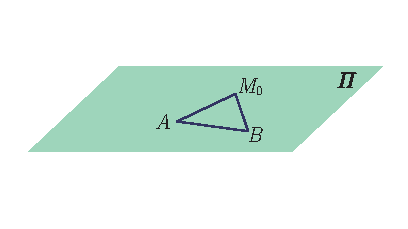
\includegraphics[width=0.9\linewidth]{picture/C-2/2.1/pm1.eps}
			%\caption{fig1}
			\label{pm1}
		\end{minipage}%
	}%
	\subfigure[定点加垂线]{
		\begin{minipage}[b]{0.33\linewidth}
			\centering
			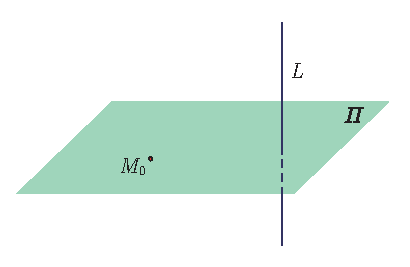
\includegraphics[width=0.9\linewidth]{picture/C-2/2.1/pm2.eps}
			%\caption{fig2}
			\label{pm2}
		\end{minipage}%
	}%
	\subfigure[外点加直线]{
		\begin{minipage}[b]{0.33\linewidth}
			\centering
			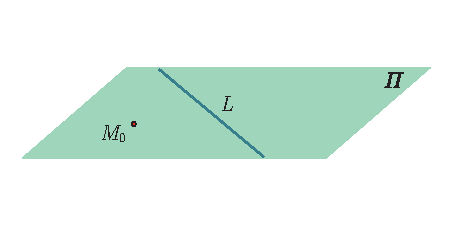
\includegraphics[width=0.95\linewidth]{picture/C-2/2.1/pm3.eps}
			%\caption{fig2}
			\label{pm3}
		\end{minipage}%
	}%
	
	\subfigure[两相交直线]{
		\begin{minipage}[b]{0.5\linewidth}
			\centering
			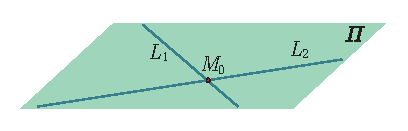
\includegraphics[width=0.9\linewidth]{picture/C-2/2.1/pm4.eps}
			%\caption{fig2}
			\label{pm4}
		\end{minipage}%
	}%
	\subfigure[两平行直线]{
		\begin{minipage}[b]{0.5\linewidth}
			\centering
			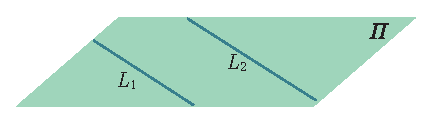
\includegraphics[width=0.9\linewidth]{picture/C-2/2.1/pm5.eps}
			%\caption{fig2}
			\label{pm5}
		\end{minipage}%
	}%
	\centering
	\caption{确定平面的条件}
\end{figure}
\newpage 
\subsection{通用的平面方程}
\begin{enumerate}[\large1.]
	\item {\color{dy}\large 坐标式方程(参数方程\index{PMFC@平面方程!CSFC@参数方程})}\index{PMFC@平面方程!ZBSFC@坐标式方程}
	\begin{enumerate}[]
		\item 已知:{\color{dl}平面上一点}:$M_0(x_0,y_0,z_0)$和平面上的{\color{dl}两个不共线的向量(直线)}:$\overrightarrow{a}=(a_1,a_2,a_3),\overrightarrow{b}=(b_1,b_2,b_3)$.
		\item 原理:三向量共面原理:$\overrightarrow{M_0M}=\lambda \overrightarrow{a}+\mu \overrightarrow{b}$.
		\item 表达式:
		\begin{equation}
		\Pi: \begin{cases}
		x=x_0+\lambda a_1+\mu b_1,\\
		y=y_0+\lambda a_2+\mu b_2,\\
		z=z_0+\lambda a_3+\mu b_3.
		\end{cases}
		\end{equation}
	\end{enumerate}
	\item {\color{dy}\large 向量式方程}\index{PMFC@平面方程!XLSFC@向量式方程}
	\begin{enumerate}[]
		\item 已知:{\color{dl}平面上一点}:$M_0(x_0,y_0,z_0)$和平面上的{\color{dl}两个不共线的向量(直线)}:$\overrightarrow{a}=(a_1,a_2,a_3),\overrightarrow{b}=(b_1,b_2,b_3)$.
		\item 原理:$\overrightarrow{OM}=\overrightarrow{OM_0}+\overrightarrow{M_0M}$,三向量共面原理.记$\overrightarrow{OM}=\overrightarrow{r},\overrightarrow{OM_0}=\overrightarrow{r_0}$.
		\item 表达式:
		\begin{equation}
		\overrightarrow{r}=\overrightarrow{r_0}+\lambda \overrightarrow{a}+\mu \overrightarrow{b}
		\end{equation}
	\end{enumerate}
	\item {\color{dy}\large 行列式方程}\index{PMFC@平面方程!HLSFC@行列式方程}
	\begin{enumerate}[]
		\item 已知:{\color{dl}平面上一点}:$M_0(x_0,y_0,z_0)$和平面上的{\color{dl}两个不共线的向量(直线)}:$\overrightarrow{a}=(a_1,a_2,a_3),\overrightarrow{b}=(b_1,b_2,b_3)$.
		\item 原理:三向量共面:$\overrightarrow{M_0M}\cdot \left( \overrightarrow{a}\times\overrightarrow{b}\right) =0$.
		\item 表达式:
		\begin{equation}
		\begin{array}{|ccc|}
		x-x_0 & y-y_0 & z-z_0 \\
		a_1 & a_2 & a_3 \\
		b_1 & b_2 & b_3
		\end{array}=0
		\label{HLS}
		\end{equation}
	\end{enumerate}
	\item {\color{dy}\large 三点式方程}\index{PMFC@平面方程!SDSFC@三点式方程}
	\begin{enumerate}[]
		\item 已知:{\color{dl}不在一条直线上的三点}:$M_1(x_1,y_1,z_1),M_2(x_2,y_2,z_2),M_3(x_3,y_3,z_3)$
		\item 原理:三向量$\overrightarrow{M_1M},\overrightarrow{M_1M_2},\overrightarrow{M_1M_3},$共面:$\overrightarrow{M_1M} \cdot \left( \overrightarrow{M_1M_2}\times\overrightarrow{M_1M_3}\right) =0$.
		\item 表达式:
		\begin{equation}
		\begin{array}{|ccc|}
		x-x_1 & y-y_1 & z-z_1 \\
		x_2-x_1 & y_2-y_1 & z_2-z_1 \\
		x_3-x_1 & y_3-y_1 & z_3-z_1
		\end{array}=0
		\end{equation}
		或
		\begin{equation}
		\begin{array}{|cccc|}
		x & y & z &1\\
		x_1&y_1 &z_1 & 1\\
		x_2& y_2 & z_2& 1\\
		x_3& y_3 & z_3&1
		\end{array}=0
		\end{equation}
		这个式子可以结合四点共面的式子\eqref{SDGM}结合记忆和理解. 
	\end{enumerate}
	\item {\color{dy}\large 一般式方程}\index{PMFC@平面方程!YBSFC@一般式方程}
	\begin{enumerate}[]
		\item 已知:{\color{dl}平面上一点}:$M_0(x_0,y_0,z_0)$和平面上的{\color{dl}两个不共线的向量(直线)}:$\overrightarrow{a}=(a_1,a_2,a_3),\overrightarrow{b}=(b_1,b_2,b_3)$.
		\item 原理:用行列式的知识按第一行展开式\eqref{HLS}.
		\item 表达式:
		\begin{equation}
		Ax+By+Cz+D=0
		\end{equation}
		其中,
		\begin{equation*}
		A=\begin{array}{|cc|}
		a_2 & a_3 \\
		b_2 & b_3
		\end{array}
		\,,\quad 
		B=\begin{array}{|cc|}
		a_3 & a_1 \\
		b_3 & b_1
		\end{array}
		\,,\quad 
		C=\begin{array}{|cc|}
		a_1 & a_2 \\
		b_1 & b_2
		\end{array}
		\,,\quad 
		D=-(Ax_0+By_0+Cz_0).
		\end{equation*}
		{\color{dy}空间任何一个平面$\Longleftrightarrow x,y,z$的三元一次方程. }
	\end{enumerate}
	
	\enbelowtheorem[向量与平面平行定理]
	\quad 设平面$\pi $的方程为
	\begin{equation*}
	Ax+By+Cz+D=0,
	\end{equation*}
	则向量$\overrightarrow{v}=(X,Y,Z)$平行于平面$\pi $的充要条件为
	\begin{equation*}
	AX+BY+CZ=0
	\end{equation*}
	
	\item {\color{dy}\large 截距式方程}\index{PMFC@平面方程!JJSFC@截距式方程}
	\begin{enumerate}[]
		\item 已知:{\color{dl}与坐标轴相交的三点}:$M_1(a,0,0),M_2(0,b,0),M_3(0,0,c)$
		\item 原理:与三点式相同,只是取与坐标轴相交的三个特殊点. 
		\item 表达式:$M_1(a,0,0),M_2(0,b,0),M_3(0,0,c)$代入三点式方程得:
		\begin{equation*}
		\begin{array}{|ccc|}
		x-a & y & z \\
		-a & b & 0 \\
		-a & 0 & c
		\end{array}=bcx+acy+abz=abc.
		\end{equation*}
		由于$abc \ne 0$,那么上式可写为:
		\begin{equation}
		\frac{x}{a}+\frac{y}{b}+\frac{z}{c}=1.
		\end{equation}
	\end{enumerate}
\end{enumerate}
\subsection{直角坐标系平面方程}
\tdefination[法向量]\index{XL@向量!FXL2@法向量}
在空间中给定一个点$M_0$和一个非零向量$\overrightarrow{n}$,那么通过点$M_0$且与向量$\overrightarrow{n}$垂直的平面是惟一确定的,我们把向量$\overrightarrow{n}$叫做这一个平面的法向量. 

\begin{enumerate}[\large1.]
	\item {\color{dy}\large 点法式方程}\index{PMFC@平面方程!DFSFC@点法式方程}
	\begin{enumerate}[]
		\item 已知:{\color{dl}一个定点}:$M_0(x_0,y_0,z_0)$和{\color{dl}一个法向量}:$\overrightarrow{n}=(A,B,C)$.如图\ref{DFS}.
		\item 原理:法向量的性质,即对于平面任意一点$M(x,y,z)$均有$\overrightarrow{MM_0}\cdot \overrightarrow{n}=0$. 
		\item 表达式:设$M_0,M$的位置矢量分别是$\overrightarrow{r_0},\overrightarrow{r}$.
		\begin{equation}
		\overrightarrow{n}\cdot\left(  \overrightarrow{r}-\overrightarrow{r_0}\right) =0
		\end{equation}
		即
		\begin{equation}
		A(x-x_0)+B(y-y_0)+C(z-z_0)+D=0
		\end{equation}
		\quad 令$D=-(Ax_0+By_0+Cz_0)$,那么上式可以表示成一般式:
		\begin{equation}
		Ax+By+Cz+D=0
		\end{equation}
	\end{enumerate}
	\begin{figure}[h]
		\centering 
		\subfigure[点法式方程]{
			\begin{minipage}[b]{0.5\linewidth}
				\centering
				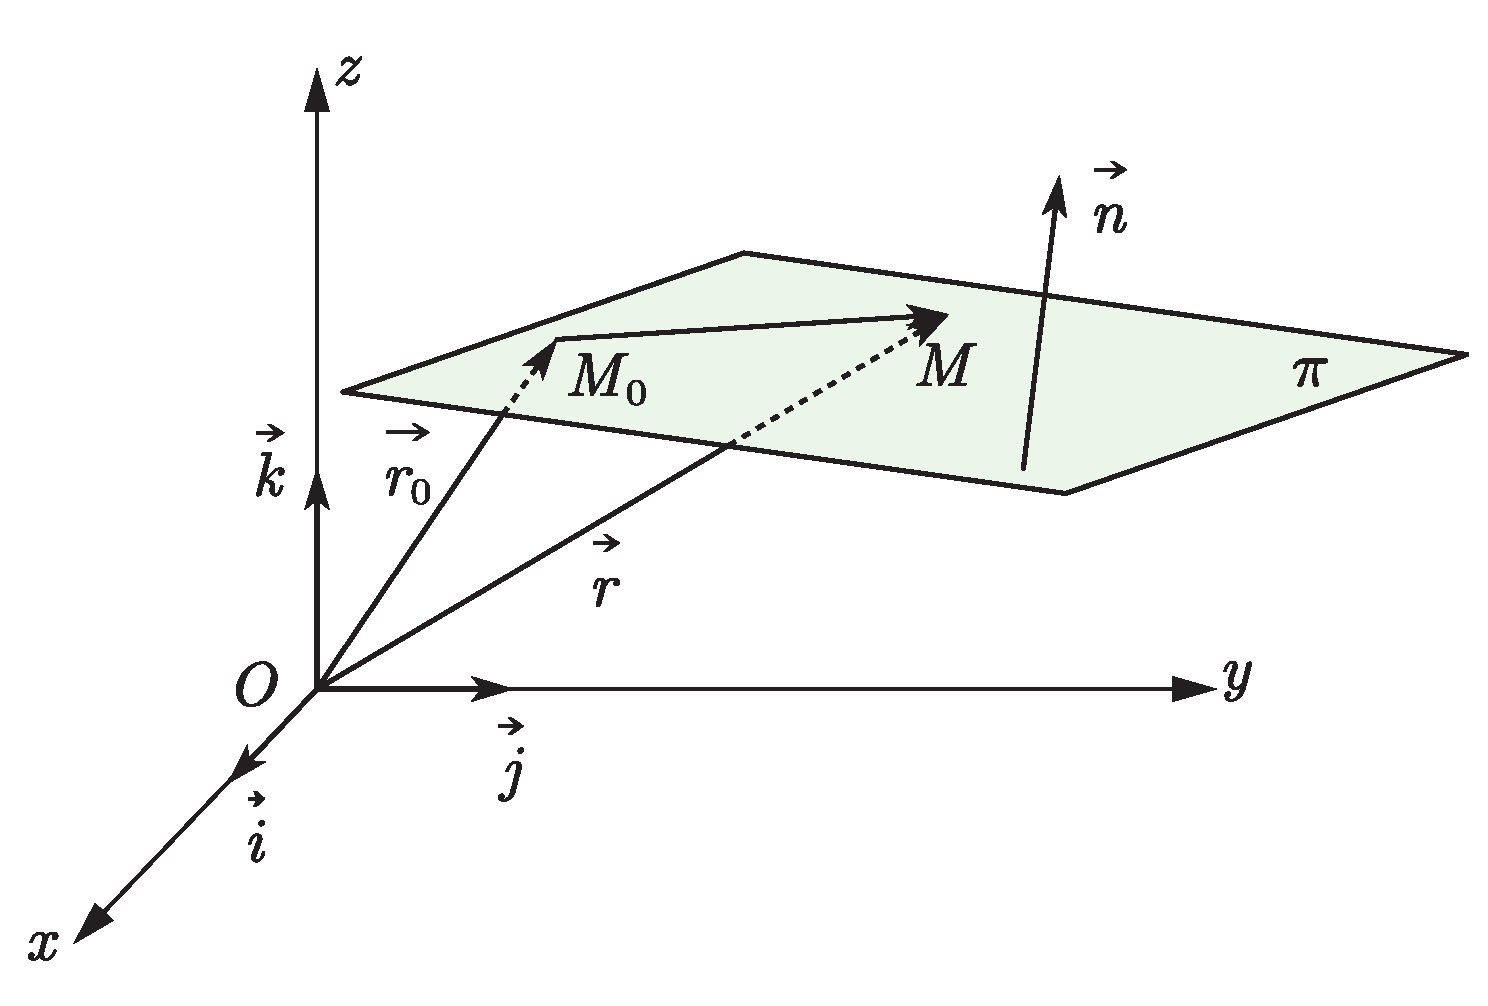
\includegraphics[width=0.9\linewidth]{picture/C-2/2.1/DFS.eps}
				%\caption{fig1}
				\label{DFS}
			\end{minipage}%
		}%
		\subfigure[向量式法式方程]{
			\begin{minipage}[b]{0.5\linewidth}
				\centering 
				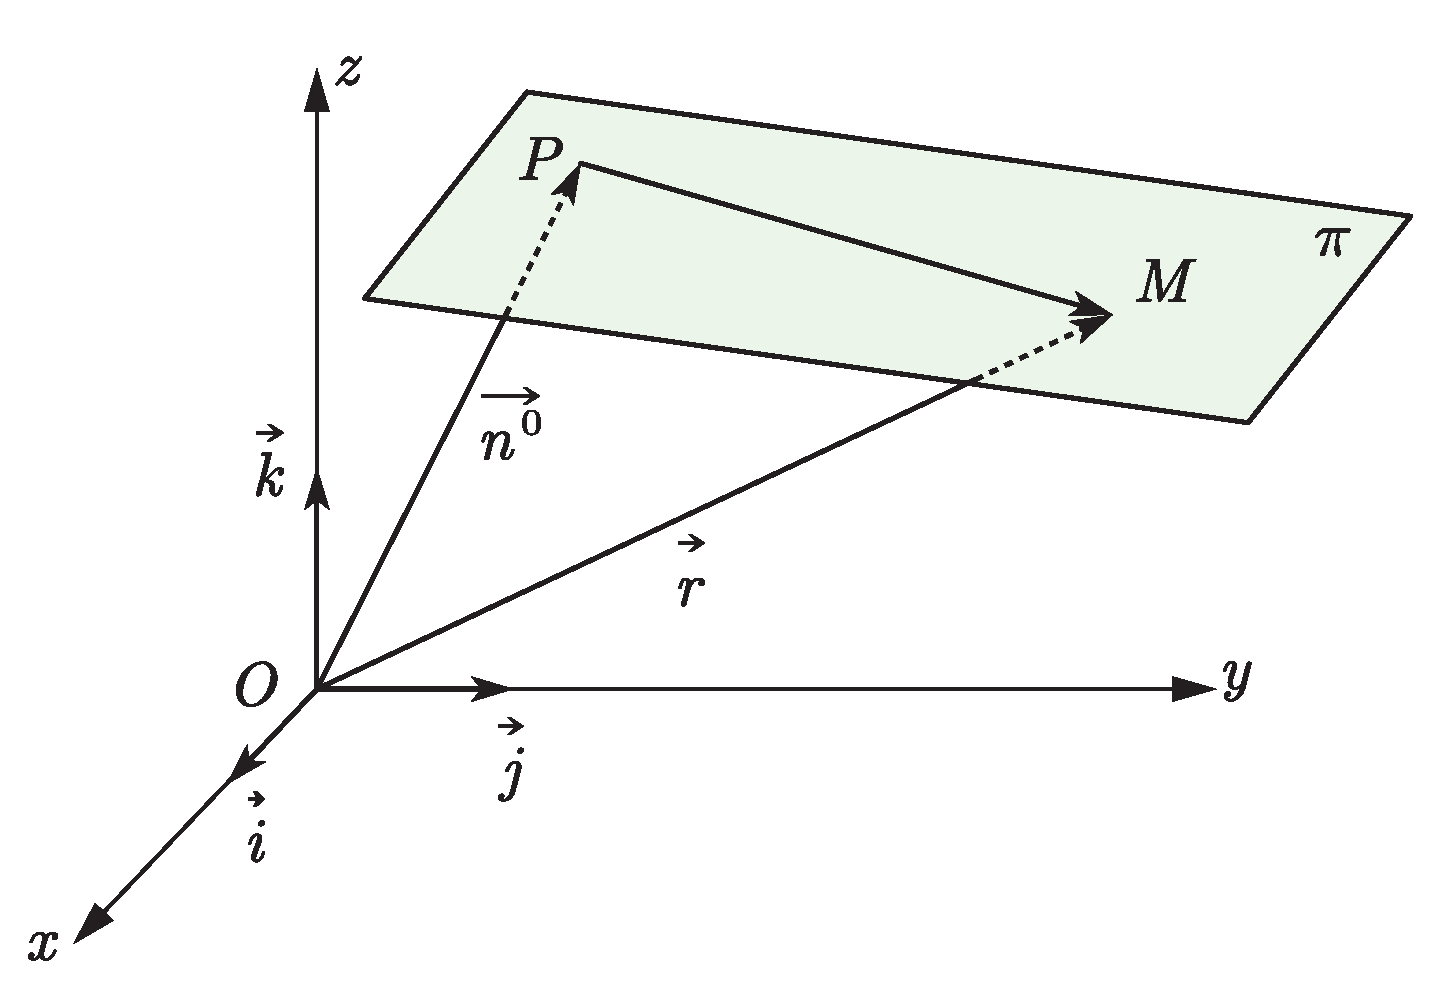
\includegraphics[width=0.9\linewidth]{picture/C-2/2.1/XLFS.eps}
				%\caption{fig2}
				\label{XLFS}
			\end{minipage}%
		}%
		\caption{直角坐标系平面方程}
	\end{figure}
	\label{平面的向量式法式方程}
	\item  {\color{dy}\large 向量式法式方程}\index{PMFC@平面方程!XLSFSFC@向量式法式方程}
	\begin{enumerate}[]
		\item 已知:{\color{dl}一个定点}:$P(x_0,y_0,z_0),$且{\color{dl}$\ \overrightarrow{OP}$垂直于平面$\pi $}.如图\ref{XLFS}.
		\item 原理:法向量的性质,取$\overrightarrow{OP}$的单位向量$\overrightarrow{n^0}$,那么向量$\overrightarrow{n^0}$是平面的单位法向量. 
		\item 表达式:设$M$的位置矢量分别是$\overrightarrow{r}$,$\left|\overrightarrow{OP} \right| =p$,则$\overrightarrow{OP} =p\overrightarrow{n^0}.$
		\begin{equation}
		\pi :\overrightarrow{n^0}\cdot \left(\overrightarrow{r}-p\overrightarrow{n^0} \right) =\overrightarrow{n^0}\cdot \overrightarrow{r}-p=0.
		\end{equation}
		\qquad 设$\overrightarrow{n^0}=\left(\cos \alpha ,\cos \beta ,\cos \gamma \right) $,其中$\alpha , \beta , \gamma$是向量$\overrightarrow{n^0}$的方向角,那么上式可以表示成\\
		{\color{dy}坐标式法式方程}:\index{PMFC@平面方程!ZBSFSFC@坐标式法式方程}
		\begin{equation}
		x\,\cos \alpha +y\,\cos \beta +z\,\cos \gamma-p=0.
		\end{equation}
	\end{enumerate}
	{\color{dy}法向量的方向规定}\\
	\hspace*{0.7cm} 如果点$P$是原点向平面$\pi $所引垂线的垂足,且法向量取单位法向量$\overrightarrow{n^0}$,那么
	\begin{enumerate}[(1)]
		\setlength{\itemindent}{3em}
		\setlength{\topsep}{0.01em}
		\setlength{\itemsep}{0.01em}
		\item 当平面不过原点时,规定$\overrightarrow{n^0}$正向与$\overrightarrow{OP}$相同,即{\color{dl}由原点指向平面};
		\item 当平面过原点时,$\overrightarrow{n^0}$正向在垂直于平面的两个方向中{\color{dl}任选一个}即可.
	\end{enumerate}
	{\color{dy}法式方程的特点}\\
	\hspace*{0.7cm} 平面的坐标式法式方程也是一种一般方程,但它满足两个条件:
	\begin{enumerate}[(1)]
		\setlength{\itemindent}{3em}
		\setlength{\topsep}{0.01em}
		\setlength{\itemsep}{0.01em}
		\item 一次项系数的平方和等于1;
		\item 常数项$-p \le 0$.
	\end{enumerate}
	{\color{dy}法式化因子}\\\index{PMFC@平面方程!XLSFSFC@向量式法式方程!FSHYZ@法式化因子}
	\hspace*{0.7cm} 要将直角坐标系下的一般方程
	\begin{equation*}
	Ax+By+Cz+D=0
	\end{equation*}
	化为法式方程,需要将法向量$\overrightarrow{n}=(A,B,C)$单位化,只要以
	\begin{equation}
	\lambda =\pm \frac{1}{|\overrightarrow{n}|}=\pm \frac{1}{\sqrt{A^2+B^2+C^2}}
	\end{equation}
	乘一般方程即可。$\lambda $的符号选取满足$\lambda D=-p \le 0.$即
	\begin{enumerate}[(1)]
		\setlength{\itemindent}{3em}
		\setlength{\topsep}{0.01em}
		\setlength{\itemsep}{0.01em}
		\item 当$D \neq 0$时,$\lambda $的符号与$D$相异;
		\item 当$D = 0$时,$\lambda $的符号可以任意选取其一.
	\end{enumerate}
	取定符号的因子$\lambda $称为平面的法式化因子.
\end{enumerate}
\section{特殊的平面方程}
对于平面一般式方程$Ax+By+Cz+D=0$,有
\begin{center}
	\begin{tabular}{|c|c|c|}
		\hline 
		条件&方程  &平面特点  \\ 
		\hline 
		$D=0$&$Ax+By+Cz=0$  & 通过原点 \\ 
		\hline 
		$A=0$&$By+Cz+D=0$  &\makecell [c]{\hspace*{0.5cm} 法向量$\overrightarrow{n}=(0,B,C)$  垂直于$x$轴,\hspace*{0.5cm} \\ \hspace*{0.5cm} 该平面平行(或包含)于$x$轴\hspace*{0.5cm} } \\ 
		\hline 
		$B=0$&$Ax+Cz+D=0$  &\makecell [c]{\hspace*{0.5cm} 法向量$\overrightarrow{n}=(A,0,C)$  垂直于$y$轴,\hspace*{0.5cm}  \\ \hspace*{0.5cm} 该平面平行(或包含)于$y$轴\hspace*{0.5cm} } \\ 
		\hline 
		$C=0$&$Ax+By+D=0$  &\makecell [c]{\hspace*{0.5cm} 法向量$\overrightarrow{n}=(A,B,0)$  垂直于$z$轴,\hspace*{0.5cm} \\ \hspace*{0.5cm} 该平面平行(或包含)于$z$轴\hspace*{0.5cm} } \\ 
		\hline 
		$A=B=0$& $\displaystyle Cz+D=0  (z=-\frac{D}{C})$ & \makecell [c]{\hspace*{0.5cm} 法向量$\overrightarrow{n}=(0,0,C)$  垂直于$x,y$轴,\hspace*{0.5cm} \\ \hspace*{0.5cm} 该平面平行(或重合)于$xOy$平面\hspace*{0.5cm} } \\ 
		\hline 
		$B=C=0$& $\displaystyle Ax+D=0 (x=-\frac{D}{A})$ & \makecell [c]{\hspace*{0.5cm} 法向量$\overrightarrow{n}=(A,0,0)$  垂直于$y,z$轴,\hspace*{0.5cm}  \\ \hspace*{0.5cm} 该平面平行(或重合)于$yOz$平面\hspace*{0.5cm} } \\ 
		\hline 
		$A=B=0$& $\displaystyle By+D=0 (z=-\frac{D}{B})$ & \makecell [c]{\hspace*{0.5cm} 法向量$\overrightarrow{n}=(0,B,0)$  垂直于$x,z$轴,\hspace*{0.5cm} \\ \hspace*{0.5cm} 该平面平行(或重合)于$xOz$平面\hspace*{0.5cm} } \\ 
		\hline 
	\end{tabular} 
\end{center}


\section{直线的方程}
\subsection{确定直线的条件}
\begin{enumerate}[$\bullet$]
	\setlength{\itemindent}{3em}
	\setlength{\topsep}{0.01em}
	\setlength{\itemsep}{0.01em}
	\item 过一定点可以作唯一直线平行于一定直线 .如图\ref{ZX1}.
	\item 两点可以确定一条直线.如图\ref{ZX2}.
	\item 任意一条直线可以视为两相交平面的交线.如图\ref{ZX3}.
\end{enumerate}
\begin{figure}[h]
	\subfigure[点和平行直线]{
		\begin{minipage}[b]{0.3\linewidth}
			\centering
			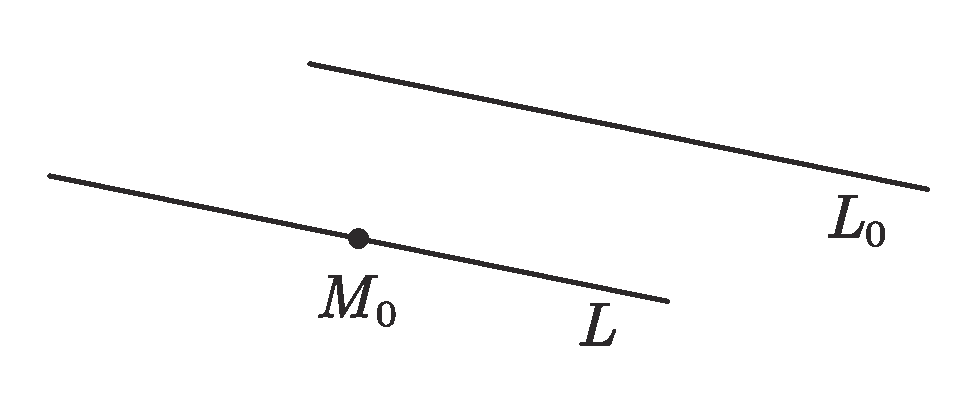
\includegraphics[width=0.9\linewidth]{picture/C-2/2.3/ZX1.pdf}
			\label{ZX1}
		\end{minipage}
	}
	\subfigure[两个不重合点]{
		\begin{minipage}[b]{0.3\linewidth}
			\centering
			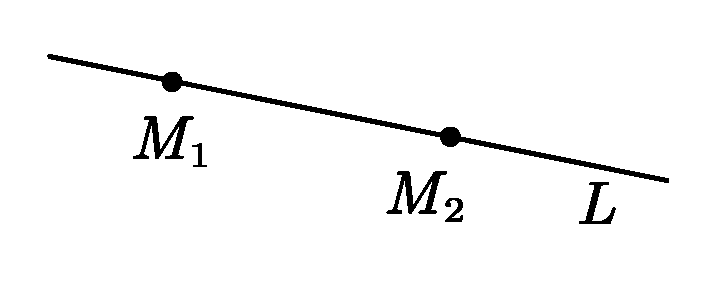
\includegraphics[width=0.9\linewidth]{picture/C-2/2.3/ZX2.pdf}
			\label{ZX2}
		\end{minipage}
	}
	\subfigure[两个相交平面]{
		\begin{minipage}[b]{0.4\linewidth}
			\centering
			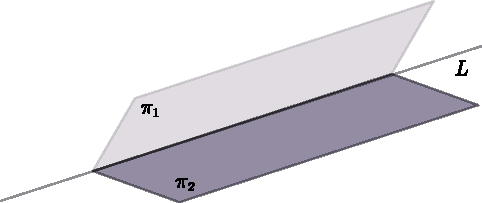
\includegraphics[width=0.9\linewidth]{picture/C-2/2.3/ZX3.pdf}
			\label{ZX3}
		\end{minipage}
	}
	\caption{确定直线的条件}
\end{figure}
\subsection{直线的通用方程}\index{ZXFC@直线方程}
\begin{enumerate}[\large1.]
	\item {\color{dy}\large 参数方程}\label{直线的参数方程}\index{ZXFC@直线方程!CSFC@参数方程}
	\begin{enumerate}[]
		\item 已知:{\color{dl}一点}:$M_0(x_0,y_0,z_0)$和{\color{dl}直线的方向向量}:$\overrightarrow{v}=(m,n,p)$.如图\ref{ZSCSFC}.
		\item 原理:过一定点可以作唯一直线平行于一定直线,直线上的所有向量都与该方平行.即
		$$\overrightarrow{M_0M}=t\overrightarrow{v}.$$
		\item 表达式:
		\begin{equation}
		L: \begin{cases}
		x=x_0+mt,\\
		y=y_0+nt,\\
		z=z_0+pt.
		\end{cases}(-\infty<t<+\infty).
		\end{equation}
		\item 特点:1.直线方程只含一个自由参数,通常说直线是一维的. \\
		2.直线可以看作匀速运动的质点轨迹,其中$\overrightarrow{v}$是速度,$t$是时间 .
	\end{enumerate}
	\begin{figure}[h]
		\subfigure[参数方程/点向式方程]{
			\begin{minipage}[b]{0.5\linewidth}
				\centering
				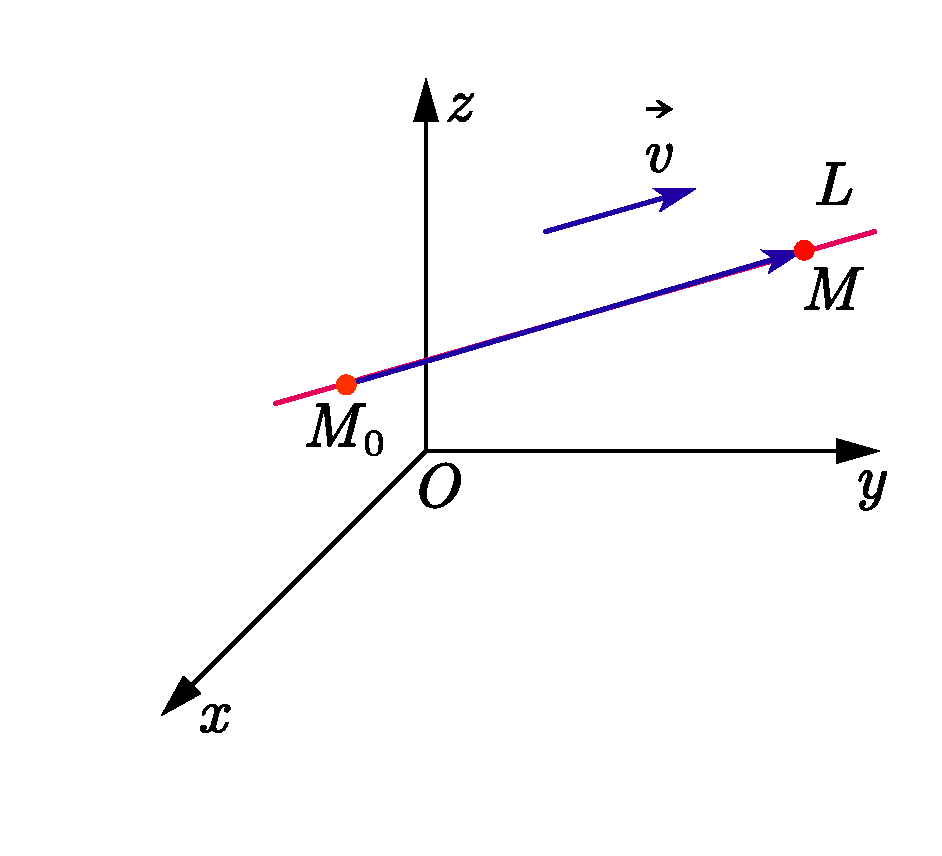
\includegraphics[width=0.9\linewidth]{picture/C-2/2.3/ZXCSFC.pdf}
				\label{ZSCSFC}
			\end{minipage}
		}
		\subfigure[向量式方程]{
			\begin{minipage}[b]{0.5\linewidth}
				\centering
				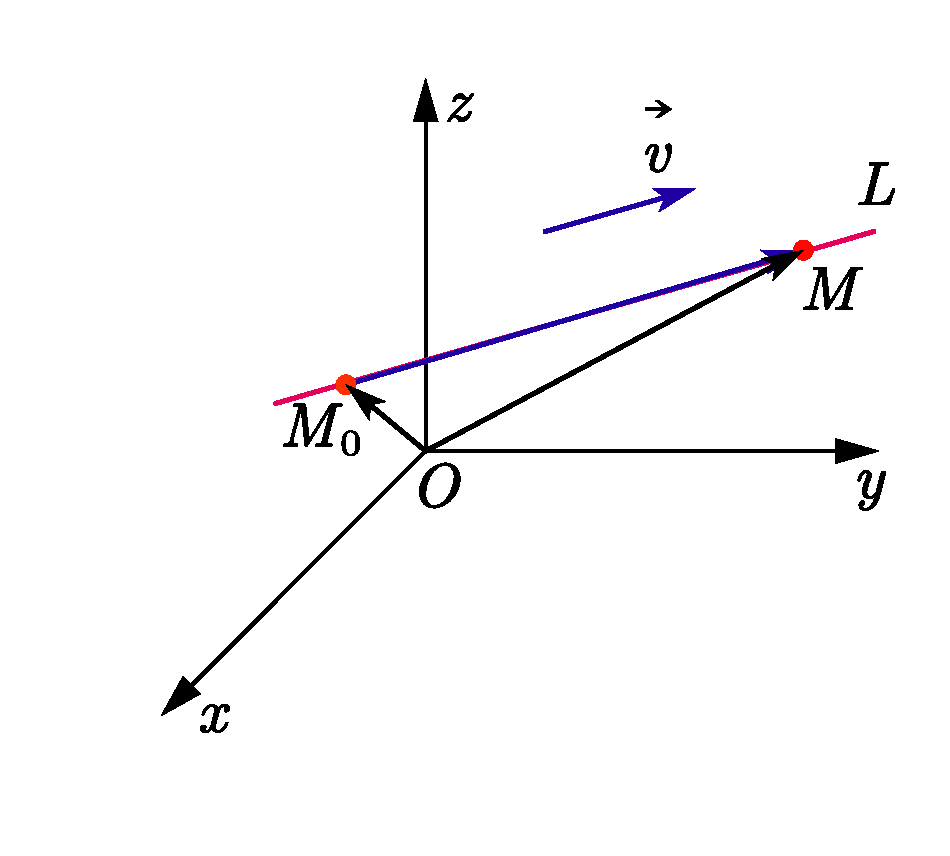
\includegraphics[width=0.9\linewidth]{picture/C-2/2.3/ZXXLSFC.pdf}
				\label{ZSXLSFC}
			\end{minipage}
		}
		\caption{直线的方程\uppercase\expandafter{\romannumeral1}}
	\end{figure}
	\item {\color{dy}\large 向量式方程}\index{ZXFC@直线方程!XLSFC@向量式方程}
	\begin{enumerate}[]
		\item 已知:{\color{dl}一点}:$M_0(x_0,y_0,z_0)$和{\color{dl}直线的方向向量}:$\overrightarrow{v}=(m,n,p)$.如图\ref{ZSXLSFC}.
		\item 原理:过一定点可以作唯一直线平行于一定直线,直线上的所有向量都与该方平行.即
		$$\overrightarrow{M_0M}=\overrightarrow{OM}-\overrightarrow{OM_0}=\overrightarrow{r}-\overrightarrow{r_0}=t\overrightarrow{v}.$$
		\item 表达式:
		\begin{equation}
		\overrightarrow{r}=\overrightarrow{r_0}+t\overrightarrow{v}
		\end{equation}
	\end{enumerate}
	\item {\color{dy}\large 点向式方程}\label{点向式方程}\index{ZXFC@直线方程!DXSFC@点向式方程}
	\begin{enumerate}[]
		\item 已知:{\color{dl}一点}:$M_0(x_0,y_0,z_0)$和{\color{dl}直线的方向向量}:$\overrightarrow{v}=(m,n,p)$.如图\ref{ZSCSFC}.
		\item 原理:$\overrightarrow{M_0M}$与方向向量$\overrightarrow{v}$平行.可以表示成
		$$\overrightarrow{M_0M}\times\overrightarrow{v}=\overrightarrow{0},\qquad  \overrightarrow{M_0M}=t\overrightarrow{v}.$$
		\item 表达式:
		\begin{equation}
		L: \frac{x-x_0}{m}=\frac{y-y_0}{n}=\frac{z-z_0}{p}
		\end{equation}
		\item 特点:点向式方程又称为{\color{dy}标准式方程}或{\color{dy}对称式方程}.
	\end{enumerate}
	\begin{figure}[h]
		\subfigure[两点式方程]{
			\begin{minipage}[b]{0.5\linewidth}
				\centering
				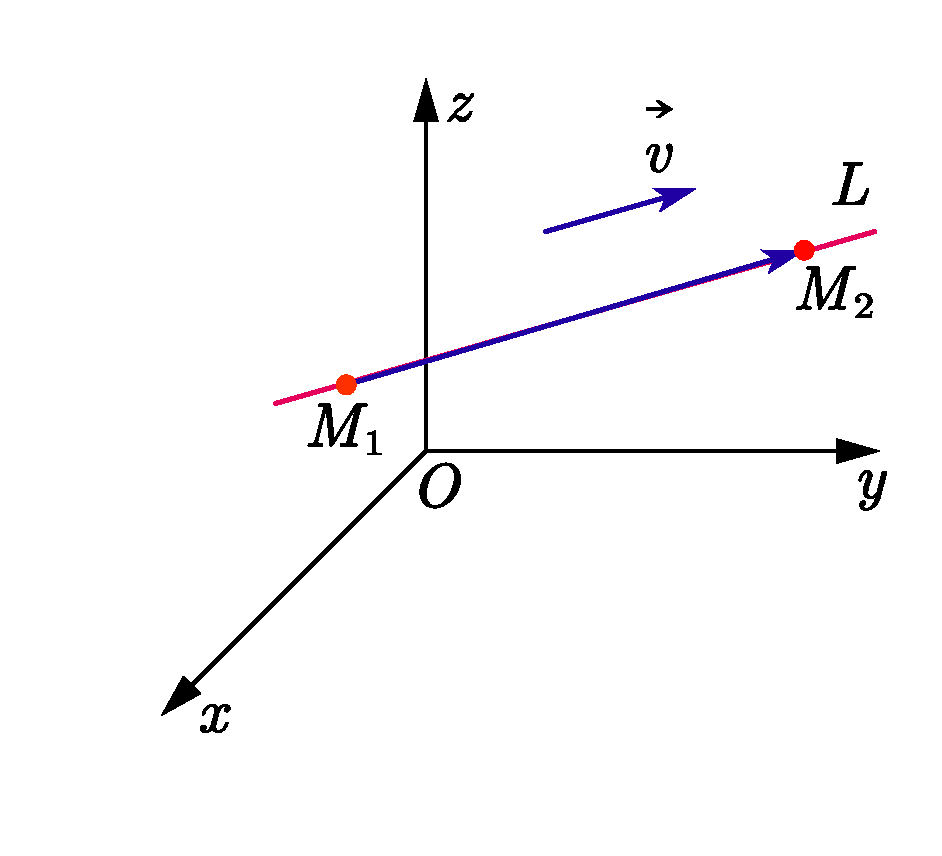
\includegraphics[width=0.9\linewidth]{picture/C-2/2.3/ZXLDSFC.pdf}
				\label{ZSLDSFC}
			\end{minipage}
		}
		\subfigure[一般式方程]{
			\begin{minipage}[b]{0.5\linewidth}
				\centering
				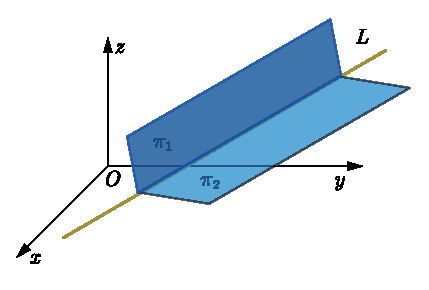
\includegraphics[width=0.9\linewidth]{picture/C-2/2.3/ZXYBFC.eps}
				\label{ZSYBFC}
			\end{minipage}
		}
		\caption{直线的方程\uppercase\expandafter{\romannumeral2}}
	\end{figure}
	\item  {\color{dy}\large 两点式方程}\label{两点式方程}\index{ZXFC@直线方程!LDSFC@两点式方程}
	\begin{enumerate}[]
		\item 已知:{\color{dl}不重合的两点}:$M_1(x_1,y_1,z_1),M_2(x_2,y_2,z_2)$.如图\ref{ZSLDSFC}.
		\item 原理:两点确定一条直线.本质上与点向式相同,即一个点$M_1(x_1,y_1,z_1)$和方向向量$\overrightarrow{v}=\overrightarrow{M_1M_2}$.
		\item 表达式:
		\begin{equation}
		L: \frac{x-x_1}{x_2-x_1}=\frac{y-y_1}{y_2-y_1}=\frac{z-z_1}{z_2-z_1}
		\end{equation}
	\end{enumerate}
	\newpage 
	\item  {\color{dy}\large 一般式方程}\index{ZXFC@直线方程!YBSFC@一般式方程}
	\begin{enumerate}[]
		\item 已知:{\color{dl}相交的两个平面}如图\ref{ZSYBFC}.
		\begin{equation*}
		\begin{cases}
		\pi_1:A_1x+B_1y+C_1z+D_1=0,\\
		\pi_2:A_2x+B_2y+C_2z+D_2=0.
		\end{cases}
		\end{equation*}
		\item 原理:任意一条直线可以视为两相交平面的交线.即联立两个平面方程.
		\item 表达式:
		\begin{equation}
		L: \begin{cases}
		\pi_1:A_1x+B_1y+C_1z+D_1=0,\\
		\pi_2:A_2x+B_2y+C_2z+D_2=0.
		\end{cases}
		\end{equation}
	\end{enumerate}
	\item  {\color{dy}\large 一般式方程转换为点向式方程}
	\begin{enumerate}[]
		\item 已知:{\color{dl}相交的两个平面}如图\ref{ZSYBFC}.
		\begin{equation*}
		\begin{cases}
		\pi_1:A_1x+B_1y+C_1z+D_1=0,\\
		\pi_2:A_2x+B_2y+C_2z+D_2=0.
		\end{cases}
		\end{equation*}
		\item 原理:直线与两个平面的法向量都垂直.叉乘后的向量与原来两个向量均垂直.
		\item 表达式:
		\begin{equation}
		\overrightarrow{v}=\overrightarrow{n_1}\times\overrightarrow{n_2}=
		\begin{array}{|ccc|}
		\overrightarrow{i} &\overrightarrow{j}  &\overrightarrow{k}  \\ 
		A_1 & B_1 & C_1 \\ 
		A_2 & B_2 & C_2
		\end{array} 
		\end{equation}
		再在两平面的交线上取一点$M_0(x_0,y_0,z_0)$即可.
	\end{enumerate}
\end{enumerate}


\section{线性图形的位置关系}
\subsection{平面与平面的位置关系}
\ttheorem[平面与平面的位置关系]
\quad 在仿射坐标系下,设两平面的方程为:
\begin{equation*}
\begin{array}{c}
\pi_1:A_1x+B_1y+C_1z+D_1=0,\\
\pi_2:A_2x+B_2y+C_2z+D_2=0.
\end{array}
\end{equation*}
那么,
\begin{enumerate}[$\mathrm (1)$]
	\setlength{\itemindent}{3em}
	\setlength{\topsep}{0.01em}
	\setlength{\itemsep}{0.01em}
	\item $\pi _1$与$\pi_2$相交于一条直线的充要条件是$\overrightarrow{n_1} \nparallel \overrightarrow{n_2} \Leftrightarrow A_1:B_1:C_1\ne A_2:B_2:C_2$.
	\item  $\pi _1$与$\pi_2$平行的充要条件是$\overrightarrow{n_1}\parallel\overrightarrow{n_2},\pi_1 \ne \pi_2 \Leftrightarrow \displaystyle \frac{A_1}{A_2}=\frac{B_1}{B_2}=\frac{C_1}{C_2} \ne \frac{D_1}{D_2}$.
	\item  $\pi _1$与$\pi_2$重合的充要条件是$\pi_1 = \pi_2 \Leftrightarrow \displaystyle \frac{A_1}{A_2}=\frac{B_1}{B_2}=\frac{C_1}{C_2}= \frac{D_1}{D_2}$.
\end{enumerate}
{\color{dy}本质:平面是否平行,法向量是平面定位的重要参考.重不重合看点,平不平行看法向量.}

\subsection{直线与直线的位置关系}
\ttheorem[直线与直线的位置关系]
\quad 在仿射坐标系下,设两直线方向向量为$\overrightarrow{v_1}=(m_1,n_1,p_1),\overrightarrow{v_2}=(m_2,n_2,p_2)$,分别过定点$M_1(x_1,y_1,z_1),M_2(x_2,y_2,z_2)$,其方程分别为:
\begin{equation*}
\begin{array}{c}
\displaystyle L_1:\frac{x-x_1}{m_1}=\frac{y-y_1}{n_1}=\frac{z-z_1}{p_1},\\
\displaystyle L_2:\frac{x-x_2}{m_2}=\frac{y-y_2}{n_2}=\frac{z-z_2}{p_2}
\end{array}
\end{equation*}
那么,记
\begin{equation*}
\Delta =\left[ \overrightarrow{v_1} \quad \overrightarrow{v_2} \quad \overrightarrow{M_1M_2}\right] =
\begin{array}{|ccc|}
m_1 & n_1 & p_1 \\ 
m_2 & n_2 & p_2 \\ 
x_2-x_1 & y_2-y_1 & z_2-z_1
\end{array} 
\end{equation*}
\begin{enumerate}[$\mathrm (1)$]
	\setlength{\itemindent}{3em}
	\setlength{\topsep}{0.01em}
	\setlength{\itemsep}{0.01em}
	\item  $L _1$与$L_2$平行的充要条件是$L_1 \parallel L_2 \Leftrightarrow \overrightarrow{v_1} \parallel \overrightarrow{v_2} \nparallel \overrightarrow{M_1M_2} \Leftrightarrow \displaystyle \frac{m_1}{m_2}=\frac{n_1}{n_2}=\frac{p_1}{p_2} \,,L_1 \ne \lambda L_2$.
	\item  $L _1$与$L_2$重合的充要条件是$L_1 \parallel L_2 \Leftrightarrow \overrightarrow{v_1} \parallel \overrightarrow{v_2} \parallel \overrightarrow{M_1M_2} \Leftrightarrow \displaystyle \frac{m_1}{m_2}=\frac{n_1}{n_2}=\frac{p_1}{p_2} \,,L_1 =\lambda L_2$.
	\item  $L _1$与$L_2$相交的充要条件是$\overrightarrow{v_1} \nparallel \overrightarrow{v_2},$且$\overrightarrow{v_1},\overrightarrow{v_2},\overrightarrow{M_1M_2}$共面$\Leftrightarrow \Delta = 0,\overrightarrow{v_1} \nparallel \overrightarrow{v_2}.$
	\item  $L _1$与$L_2$异面的充要条件是$\overrightarrow{v_1},\overrightarrow{v_2},\overrightarrow{M_1M_2}$不共面$\Leftrightarrow \Delta \ne  0.$
\end{enumerate}



\subsection{直线与平面的位置关系}
\ttheorem[直线与平面的位置关系]
\quad 在{\color{dy}直角坐标系}下,设法向量为$\overrightarrow{n}=(A,B,C)$的平面和过点$M_0(x_0,y_0,z_0)$且方向向量为$\overrightarrow{v}$的直线方程分别为:
\begin{equation*}
\begin{array}{c}
\pi:Ax+By+Cz+D=0,\\
\displaystyle L:\frac{x-x_0}{m}=\frac{y-y_0}{n}=\frac{z-z_0}{p}.
\end{array}
\end{equation*}
那么,
\begin{enumerate}[$\mathrm (1)$]
	\setlength{\itemindent}{3em}
	\setlength{\topsep}{0.01em}
	\setlength{\itemsep}{0.01em}
	\item  平面$\pi $与直线$L$平行的充要条件是$\overrightarrow{n} \perp \overrightarrow{v} \Leftrightarrow Am+Bn+Cp=0.$
	\item  平面$\pi $与直线$L$重合的充要条件是$\overrightarrow{n}  \perp \overrightarrow{v}$且$M_0(x_0,y_0,z_0)$在平面$\pi $上$\Leftrightarrow Am+Bn+Cp=0,Ax_0+By_0+Cz_0+D=0.$
	\item  平面$\pi $与直线$L$相交的充要条件是$\overrightarrow{n}  \not \perp \overrightarrow{v} \Leftrightarrow Am+Bn+Cp \neq 0.$
	\item  特别地,平面$\pi $与直线$L$垂直的充要条件是$\overrightarrow{n} \parallel  \overrightarrow{v} \Leftrightarrow \displaystyle \frac{A}{m}=\frac{B}{n}=\frac{C}{p}.$
\end{enumerate}



\subsection{平面束方程}\index{PMSFC@平面束方程}
\tdefination[定线平面束]\index{PMSFC@平面束方程!DXPMS@定线平面束}
过一条定直线的所有平面的集合称为{\color{dy}平面束方程},过直线
\begin{equation*}
L:
\begin{cases}
A_1x+B_1y+C_1z+D_1=0\\
A_2x+B_2y+C_2z+D_2=0
\end{cases}
\end{equation*}
的平面束方程为
\begin{equation}
\pi:\mu \left( A_1x+B_1y+C_1z+D_1\right) +\lambda \left( A_2x+B_2y+C_2z+D_2\right)=0.\quad (-\infty \leq \lambda ,\mu \leq +\infty)
\end{equation}


\defination[平行平面束]\index{PMSFC@平面束方程!PXPMS@平行平面束}
平行于平面$\pi :Ax+By+Cz+D=0$所有平面的集合称为{\color{dy}平行平面束方程},即表示为
\begin{equation}
Ax+By+Cz+D‘=0\quad (D' \neq D)
\end{equation}



\section{线性图形的距离}
\subsection{点到直线的距离}
\ttheorem[点到直线的距离]
在{\color{dy}直角坐标系}中,点$M(x,y,z)$到过定点$M_0(x_0,y_0,z_0)$,且方向向量为$\overrightarrow{v}=(m,n,p)$的直线
\begin{equation*}
L: \frac{x-x_0}{m}=\frac{y-y_0}{n}=\frac{z-z_0}{p}
\end{equation*}
的距离为:
\begin{equation}
d=\frac{|\overrightarrow{MM_0} \times \overrightarrow{v}|}{\left| \overrightarrow{v}\right| }.
\end{equation}


\subsection{离差}
\tdefination[离差]
\quad 如果从点$N$向平面$\pi $引垂线,垂足为点$M$,那么向量$\overrightarrow{MN}$在平面$\pi $上单位向量$\overrightarrow{n^0}$的射影叫做点$N$到平面$\pi $上的{\color{dy}离差},\index{LC@离差}记为:$\delta =\mathrm{Prj}_{\overrightarrow{n^0}}\overrightarrow{MN}.$

\noindent {\color{dy}离差的几何意义} 
\begin{enumerate}
	\item {\color{dy}\textbf{方向}}\quad 当点$N$位于平面$\pi $的单位法向量$\overrightarrow{n^0}$所指向的一侧时,离差$\delta >0$(即$\overrightarrow{MN}$与$\overrightarrow{n^0}$同向)\\
	当点$N$位于平面$\pi $的单位法向量$\overrightarrow{n^0}$所指向的另一侧时,离差$\delta <0$(即$\overrightarrow{MN}$与$\overrightarrow{n^0}$反向).
	\item {\color{dy}\textbf{大小}}\quad 离差的绝对值$|\delta| $等于点$N$到平面$\pi $的距离$d$.
\end{enumerate}
\theorem[点与平面的位置关系]
\quad 设平面$\pi $的向量法式方程为
\begin{equation*}
\pi :\overrightarrow{n^0}\cdot \overrightarrow{r}-p=0.\quad \mbox{或} \quad  x\cos \alpha+y\cos \beta +z\cos \gamma-p=0 
\end{equation*}
其中,$\overrightarrow{n^0}$为平面$\pi $的单位法向量,$p$为原点到平面$\pi $的距离.\\
\quad 则点$M_0(x_0,y_0,z)$关于平面$\pi $的离差为
\begin{equation}
\delta =x_0\cos \alpha+y_0\cos \beta +z_0\cos \gamma-p=\frac{Ax_0+By_0+Cz_0+D}{\sqrt{A^2+B^2+C^2}}
\end{equation}
因此,我们可以借此判断点$M_0$在平面$\pi $的位置(假设$\overrightarrow{n^0}$指向平面$\pi $上方):
\begin{enumerate}[$\mathrm (1)$]
	\setlength{\itemindent}{3em}
	\setlength{\topsep}{0.01em}
	\setlength{\itemsep}{0.01em}
	\item $Ax_0+By_0+Cz_0+D>0 \Longleftrightarrow $点$M_0$在平面$\pi $上方;
	\item $Ax_0+By_0+Cz_0+D=0 \Longleftrightarrow $点$M_0$在平面$\pi $内;
	\item $Ax_0+By_0+Cz_0+D<0 \Longleftrightarrow $点$M_0$在平面$\pi $下方.
\end{enumerate}



\subsection{点到平面的距离}
\ttheorem[点到平面的距离]
\quad 在{\color{dy}直角坐标系}中,点$P_1(x_1,y_1,z_1)$到平面\\
\begin{minipage}{0.6\linewidth}
	$$\pi : Ax+By+Cz+D=0$$
	的距离为:
	\begin{equation}
	d=\frac{\left| Ax_1+By_1+Cz_1+D\right| }{\sqrt{A^2+B^2+C^2}}
	\end{equation}
\end{minipage}
\hfill
\begin{minipage}{0.4\linewidth}
	\centering
	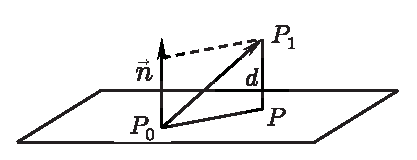
\includegraphics[scale=1]{picture/C-2/2.5/point.eps}
\end{minipage}
证明思路:利用向量在平面法向量上的投影. 如图,
$$d=\frac{\left| \overrightarrow{P_0P_1} \cdot \overrightarrow{n}\right| }{\left| \overrightarrow{n}\right| }=\frac{|(Ax_1+By_1+Cz_1)-(Ax+By+Cz+D)+D|}{\sqrt{A^2+B^2+C^2}}=\frac{\left| Ax_1+By_1+Cz_1+D\right| }{\sqrt{A^2+B^2+C^2}}$$



\subsection{平面到平面的距离}
\ttheorem[平面到平面的距离]
\quad 两平行平面$\pi _1:Ax+By+Cz+D_1=0,\pi _2:Ax+By+Cz+D_2=0(D_1 \neq D_2)$的距离为:
\begin{equation}
d=\frac{\left| D_1-D_2\right| }{\sqrt{A^2+B^2+C^2}}
\end{equation}

证明思路:在其中一个平面上任取一点即变成点到平面的距离求解。
\subsection{两直线的公垂线}
\tdefination[公垂线段]
分别与两条异面直线$l_1,l_2$垂直相交的直线$l$叫做$l_1,l_2$的公垂线\index{GCX@公垂线},两垂足的连线称为公垂线段\index{GCXD@公垂线段}。


\theorem[两直线的公垂线]
\quad 两异面直线$l_1,l_2$分别过点$M_1(x_1,y_1,z_1),M_2(x_2,y_,2z_2)$,且方向向量分别为$\overrightarrow{v_1}=(m_1,n_1,p_1),\overrightarrow{v_2}=(m_2,n_2,p_2)$.即
\begin{equation*}
\begin{array}{c}
\displaystyle l_1:\frac{x-x_1}{m_1}=\frac{y-y_1}{n_1}=\frac{z-z_1}{p_1},\\
\displaystyle l_2:\frac{x-x_2}{m_2}=\frac{y-y_2}{n_2}=\frac{z-z_2}{p_2}
\end{array}
\end{equation*}
\qquad 那么公垂线的方向向量可取$\overrightarrow{v_1} \times \overrightarrow{v_2} \neq 0$,设公垂线上一点$M(x,y,z)$,那么由$\overrightarrow{M_1M},\overrightarrow{v_1},\overrightarrow{v}$可确定一个平面$\pi_1$。同理,$\overrightarrow{M_2M},\overrightarrow{v_2},\overrightarrow{v}$可确定一个平面$\pi_2$,而公垂线就是这两个平面的交线,即
\begin{equation}
\begin{cases}
\left( \overrightarrow{r_M}-\overrightarrow{r_{M_1}}\,,\,\overrightarrow{v_1}\,,\,\overrightarrow{v}\right) =0\\
\left( \overrightarrow{r_M}-\overrightarrow{r_{M_2}}\,,\,\overrightarrow{v_2}\,,\,\overrightarrow{v}\right) =0
\end{cases}
\end{equation}
用坐标表示,得
\begin{equation}
\begin{cases}
\,
\begin{array}{|ccc|}
x-x_1 &y-y_1  &z-z_1  \\ 
m_1&n_1  &p_1  \\ 
m&n  &p 
\end{array}=0\\ 
\quad \\
\,
\begin{array}{|ccc|}
x-x_2 &y-y_2  &z-z_2  \\ 
m_2&n_2  &p_2  \\ 
m&n  &p 
\end{array}=0
\end{cases}
\end{equation}


\subsection{直线到直线的距离}
\begin{enumerate}[\large1.]
	\item {\color{dy}\large 异面直线情形}
	
	\enbelowtheorem[异面直线的距离]
	\quad 设两条异面直线$l_1,l_2$分别过点$M_1,M_2$,方向向量分别为$\overrightarrow{v_1},\overrightarrow{v_2}$,则$l_1,l_2$之间的距离为
	\begin{equation}
	d=\frac{\left| \left( \overrightarrow{M_1M_2}\,,\,\overrightarrow{v_1}\,,\,\overrightarrow{v_2}\right) \right| }{\left| \overrightarrow{v_1} \times \overrightarrow{v_2}\right|}.
	\end{equation}
	证明思路:两条异面直线$l_1,l_2$之间的距离$d$可以理解为以$\overrightarrow{M_1M_2}\,,\,\overrightarrow{v_1}\,,\,\overrightarrow{v_2}$为棱的平行六面体的体积(利用\hyperref[混合积的几何意义]{\color{超链接}混合积的几何意义}\footnote{总结的超链接均用{\color{超链接}此颜色}表示})除以$\overrightarrow{v_1}\,,\,\overrightarrow{v_2}$为邻边的平行四边形的面积(利用\hyperref[外积的几何意义]{\color{超链接}叉乘的几何意义}).
	
	
	\item {\color{dy}\large 平行直线情形}
	\begin{enumerate}[]
		\item 在任意一条直线上取一点,转换成点到直线的问题解决。
	\end{enumerate}
\end{enumerate}

\section{线性图形的夹角}
\subsection{平面与平面的夹角}
\quad 两个{\color{dy}平面的夹角}是指两个平面变成两个相邻的二面角中中任一个. 其中一个等于两个法向量的夹角.如图\ref{平面与平面的夹角}.\\

\theorem[平面与平面的夹角]
\quad 设在{\color{dy}直角坐标系}中,两个平面$\pi_1 \pi_2$的方程分别为:
\begin{equation*}
\begin{array}{c}
\pi_1:A_1x+B_1y+C_1z+D_1=0,\\
\pi_2:A_2x+B_2y+C_2z+D_2=0.
\end{array}
\end{equation*}
则$\pi_1$与$ \pi_2$的一个夹角 $\theta $满足:
\begin{equation}
\cos \theta =\frac{\overrightarrow{n_1}\cdot \overrightarrow{n_2}}{\left| \overrightarrow{n_1}\right| \left|  \overrightarrow{n_2}\right| }
=\frac{A_1A_2+B_1B_2+C_1C_2}{\sqrt{A_1^2+B_1^2+C_1^2}\cdot \sqrt{A_2^2+B_2^2+C_2^2}}
\end{equation}
那么由此可以知道两个平面$\pi_1 \pi_2$垂直的充要条件为:
\begin{equation}
A_1A_2+B_1B_2+C_1C_2=0.
\end{equation}


\begin{figure}[h]
	\subfigure[平面与平面的夹角]{
		\begin{minipage}[b]{0.4\linewidth}
			\centering
			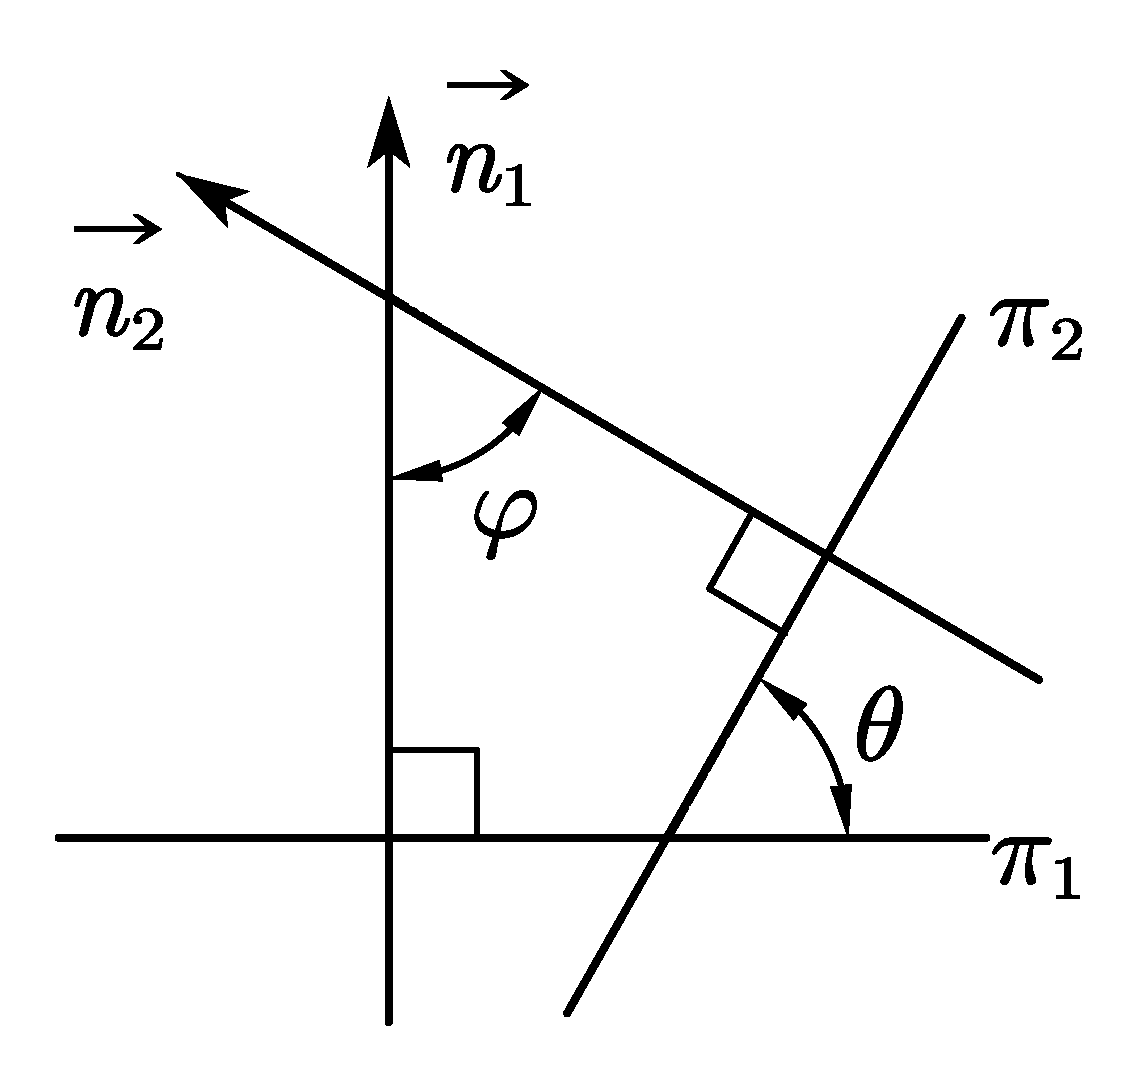
\includegraphics[width=0.7\linewidth]{picture/C-2/2.6/JJ1.pdf}
			\label{平面与平面的夹角}
		\end{minipage}
	}
	\subfigure[两直线夹角]{
		\begin{minipage}[b]{0.2\linewidth}
			\centering
			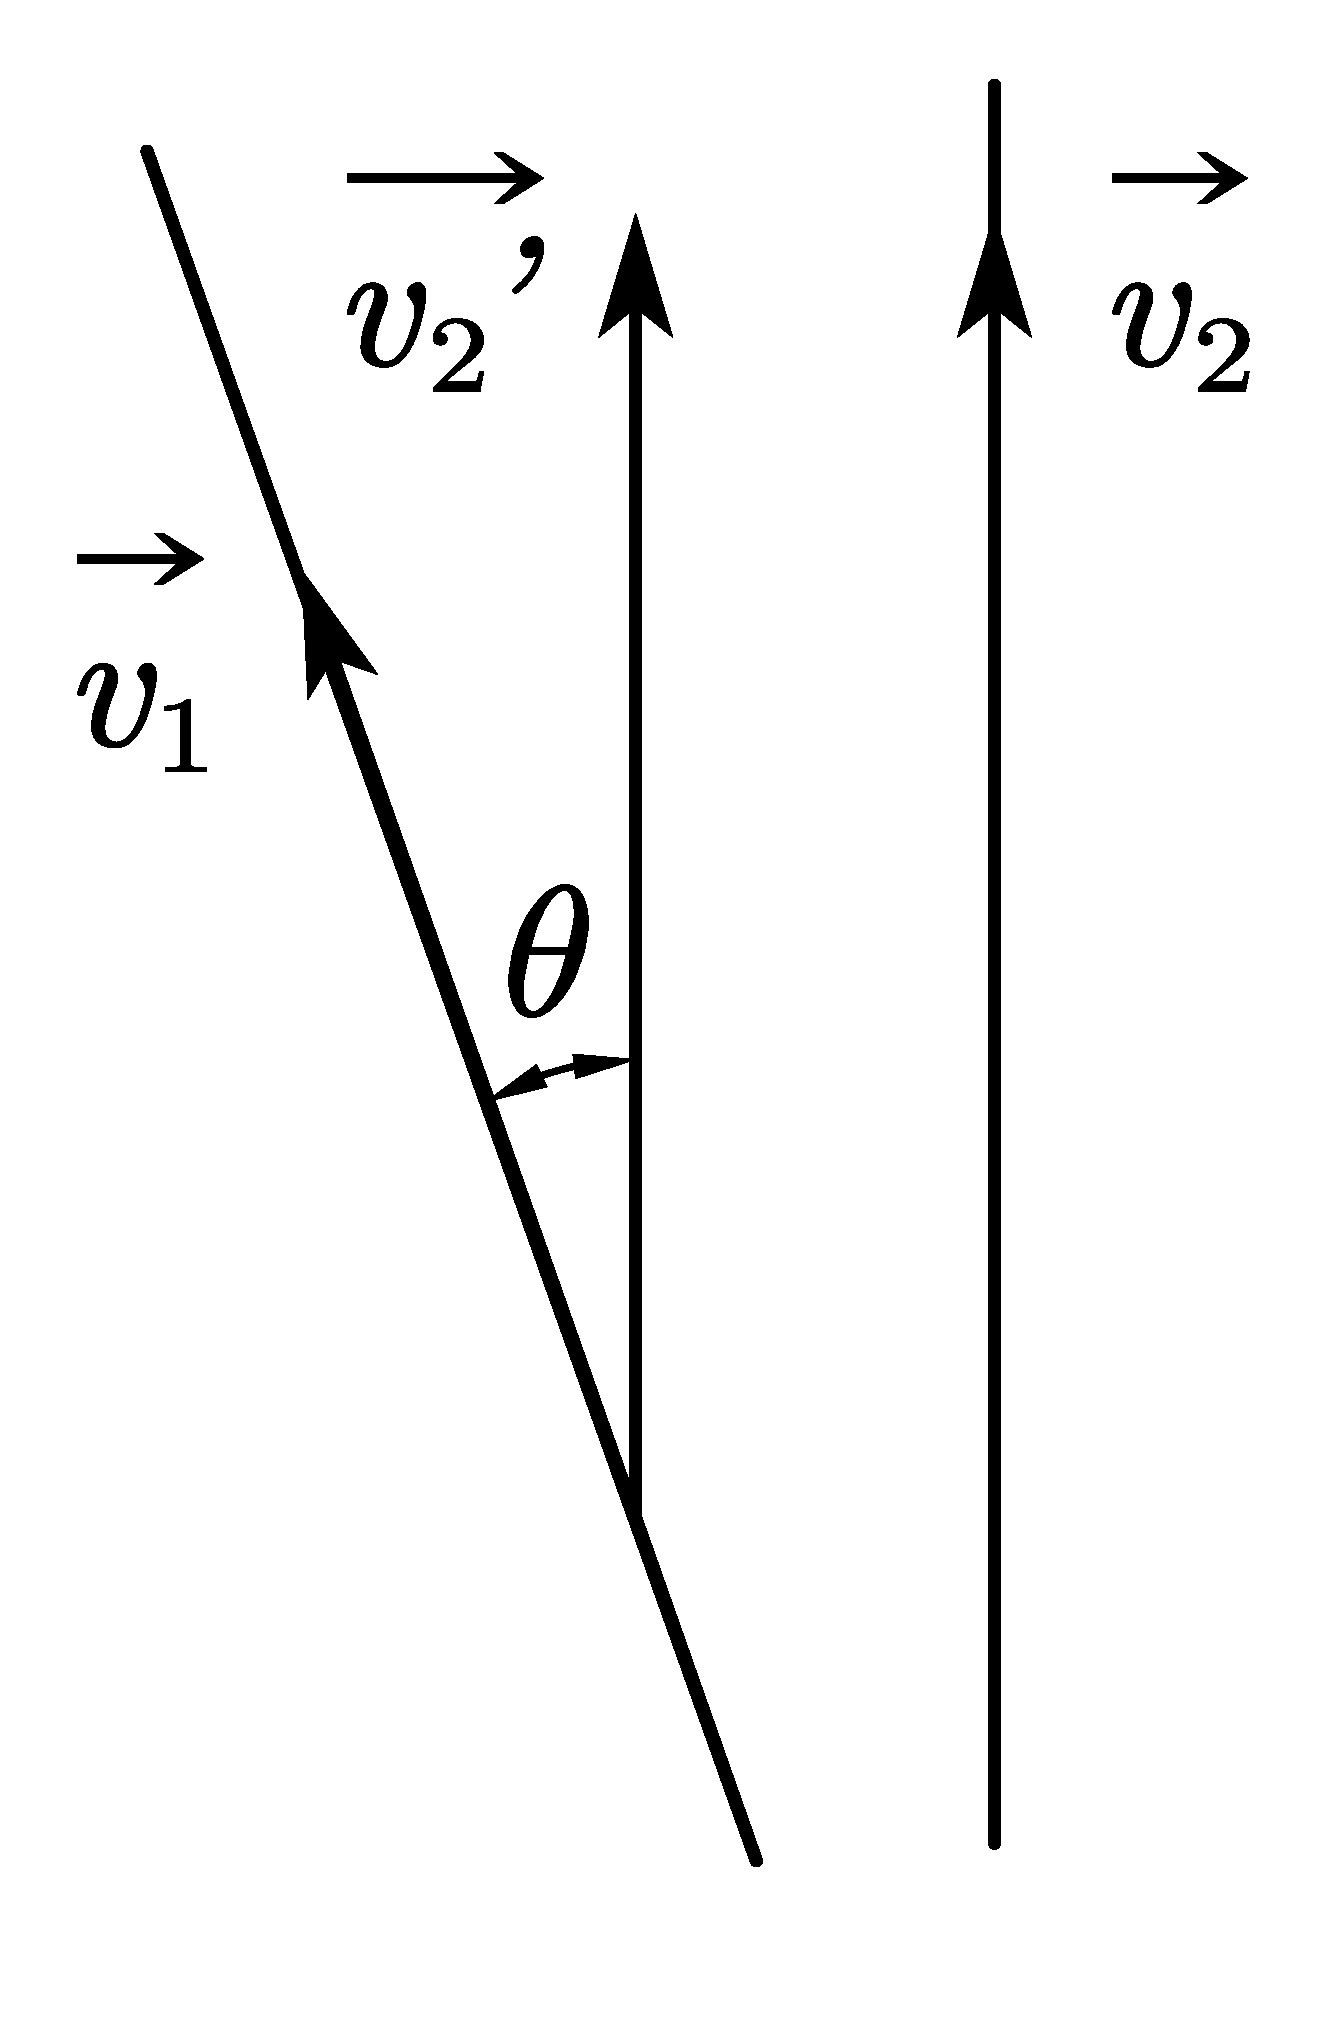
\includegraphics[width=0.8\linewidth]{picture/C-2/2.6/JJ2.pdf}
			\label{两直线的夹角}
		\end{minipage}
	}
	\subfigure[直线和平面的夹角]{
		\begin{minipage}[b]{0.4\linewidth}
			\centering
			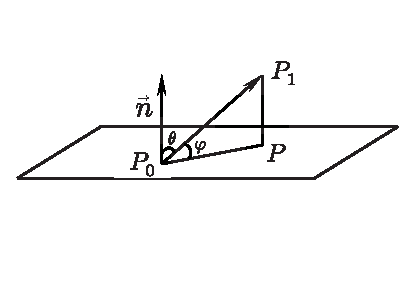
\includegraphics[width=0.9\linewidth]{picture/C-2/2.6/JJ3.eps}
			\label{直线和平面的夹角}
		\end{minipage}
	}
						\caption{线性图形的夹角}
\end{figure}
\subsection{两直线的夹角}
\quad 两条{\color{dy}直线的夹角}是指它们的方向向量的夹角或其补角.如图\ref{两直线的夹角}.

\theorem[两直线的夹角]
\quad 设在{\color{dy}直角坐标系}中,两条直线$L_1,L_2$的方向向量分别为:$\overrightarrow{v_1}=(m_1,n_1,p_1),\overrightarrow{v_2}=(m_2,n_2,p_2).$则$L_1,L_2$的夹角为$\left\langle \overrightarrow{v_1},\overrightarrow{v_2}\right\rangle $或$\pi -\left\langle \overrightarrow{v_1},\overrightarrow{v_2}\right\rangle ,$则
\begin{equation}
\begin{split}
\cos \left\langle L_1,L_2\right\rangle &=\pm \cos \left\langle \overrightarrow{v_1},\overrightarrow{v_2}\right\rangle =\pm \frac{\overrightarrow{v_1}\cdot \overrightarrow{v_2}}{|\overrightarrow{v_1}|\cdot |\overrightarrow{v_2}|}\\
&=\pm \frac{m_1m_2+n_1n_2+p_1p_2}{\sqrt{m_1^2+n_1^2+p_1^2}\cdot \sqrt{m_2^2+n_2^2+p_2^2}}
\end{split}
\end{equation}


特别地,直线$L_1,L_2$垂直的充分必要条件是:
\begin{equation}
m_1m_2+n_1n_2+p_1p_2=0
\end{equation}

\subsection{直线与平面的夹角}
\quad 当直线和平面垂直时,{\color{dy}直线与平面的夹角}是指这条直线和它在平面上的垂直射影所构成的{\color{dy2}锐角}。当直线垂直于平面时,规定{\color{dy}直线与平面的夹角}为{\color{dy2}直角}。如图\ref{直线和平面的夹角}.

\theorem[直线与平面的夹角]
\quad 设在{\color{dy}直角坐标系}中,直线$L$的方向向量为:$\overrightarrow{v}=(m,n,p).$平面$\pi $的法向量$\overrightarrow{n}=(X,Y,Z)$,设直线$L$与平面$\pi $的夹角为$\varphi \in \displaystyle \left[ 0,\frac{\pi }{2} \right],\left\langle \overrightarrow{v},\overrightarrow{n}\right\rangle =\theta \in \displaystyle \left[ 0,\pi  \right]$,则由图\ref{直线和平面的夹角}.可知:
$$\varphi =\left| \frac{\pi }{2}-\theta \right| $$
即
\begin{equation}
\begin{split}
\sin \varphi &=|\cos \theta |=\frac{|\overrightarrow{n} \cdot \overrightarrow{v} |}{|\overrightarrow{n}| \cdot |\overrightarrow{v}|}\\
&=\frac{\left| mX+nY+pZ\right| }{\sqrt{X^2+Y^2+Z^2}\,\cdot \,\sqrt{m^2+n^2+p^2}}.
\end{split}
\end{equation} 



%第三章

\chapter{常见的曲面}
\section{曲面及其方程}
\subsection{曲面的方程的定义}
\noindent
\thispagestyle{empty}
\begin{enumerate}[]
	\setlength{\itemindent}{1em}
	\setlength{\topsep}{0.01em}
	\setlength{\itemsep}{0.01em}
	\item 从几何上看,曲面可以看作是具有{\color{dy}某种约束的点的几何轨迹};
	\item 从解析上看,约束条件通常用一个{\color{dy}三元二次方程$S:F(x,y,z)=0$}表示.
\end{enumerate}
\defination[曲面的方程]\index{QMDFC@曲面的方程}
曲面$S$表示为点的集合:
\begin{equation}
S=\left\lbrace (x,y,z)\in \mathbb{R}^3|F(x,y,z)=0\right\rbrace 
\end{equation}
\par 其特点为:
\begin{enumerate}[(1)]
	\setlength{\itemindent}{3em}
	\setlength{\topsep}{0.01em}
	\setlength{\itemsep}{0.01em}
	\item 曲面上的点都满足方程;
	\item 满足方程的点都在曲面上,不满足方程的点都不在曲面上.
\end{enumerate}
\subsection{曲面方程举例}
\begin{enumerate}[1.]
	\setlength{\topsep}{0.01em}
	\setlength{\itemsep}{0.01em}
	\item {\color{dy}平面\index{PM@平面}}
	\begin{enumerate}[(1)]
		\setlength{\topsep}{0.01em}
		\setlength{\itemsep}{0.01em}
		\item 约束条件:动点到定点的连线始终与一定直线垂直。
		\item 一般方程:$Ax+By+Cz+D=0.$
	\end{enumerate}
	\item {\color{dy}球面\index{QM@球面}}\label{球面}
	\begin{enumerate}[(1)]
		\setlength{\topsep}{0.01em}
		\setlength{\itemsep}{0.01em}
		\item 约束条件:动点($M(x,y,z)$)到定点(球心$M_0(x_0,y_0,z_0)$)的距离始终为常数(半径$R$)。
		\item 一般方程:$(x-x_0)^2+(y-y_0)^2+(z-z_0)^2=R^2.$
	\end{enumerate}
	\newpage
	\item {\color{dy}圆柱面\index{YZM@圆柱面}}\label{圆柱面}
	\begin{enumerate}[(1)]
		\setlength{\topsep}{0.01em}
		\setlength{\itemsep}{0.01em}
		\item 约束条件:到一定直线的距离等于常数($R$)的动点的轨迹方程。
		\item 定直线为$z$轴的方程:$x^2+y^2=R^2.$
	\end{enumerate}
	\item {\color{dy}圆锥面\index{YZM@圆锥面}}\label{圆锥面}
	\begin{enumerate}[(1)]
		\setlength{\topsep}{0.01em}
		\setlength{\itemsep}{0.01em}
		\item 约束条件:动点与一定直线上某定点的连线始终与该定直线交成等角$\varphi $。
		\item 定直线$z$轴,其上的定点为原点的方程:$z^2=\cot^2 \varphi(x^2+y^2).$
	\end{enumerate}
\end{enumerate}
\subsection{曲面的两个基本问题}
\begin{enumerate}[1.]
	\setlength{\itemindent}{2em}
	\setlength{\topsep}{0.01em}
	\setlength{\itemsep}{0.01em}
	\item 已知曲面作为点的几何轨迹时,求曲面方程;
	\item 已知一个三元方程$F(x,y,z)=0,$研究它所表示的几何形状.
\end{enumerate}

\subsection{构建曲面方程的一般步骤}
\begin{enumerate}[1.]
	\setlength{\itemindent}{2em}
	\setlength{\topsep}{0.01em}
	\setlength{\itemsep}{0.01em}
	\item 针对实际问题,{\color{dy}建立合适的空间直角坐标系};
	\item 先在曲面上任取一{\color{dy}动点$M(x,y,z)$},再依据题意,{\color{dy}找到约束条件,建立等量关系},(即利用数学解析语言描述几何约束条件)得到{\color{dy}关于动点$M$的坐标变量$x,y,z$的等式};
	\item 整理得到{\color{dy}曲面的方程}.
\end{enumerate}

\subsection{柱坐标与球坐标}
\label{柱坐标}
\noindent
\tdefination[柱坐标]\index{ZZB@柱坐标}
空间直角坐标系中点$M(x,y,z).$
\begin{enumerate}[(1)]
	\setlength{\itemindent}{3em}
	\setlength{\topsep}{0.01em}
	\setlength{\itemsep}{0.01em}
	\item 它在$xOy$面上的投影点$N(x,y,0)$;
	\item 用极坐标系表示点$N(\rho ,\theta ,0)$.
\end{enumerate}
\par 那么我们称三元有序数组$(\rho ,\theta ,z)$为点$M$的{\color{dy}柱坐标}.如图\ref{柱坐标1}.
\begin{enumerate}[]
	\setlength{\topsep}{0.01em}
	\setlength{\itemsep}{0.01em}
	\item {\color{dy}柱坐标与直角坐标的关系}
	\begin{equation}
	\begin{cases}
	x=\rho \cos\theta,\\
	y=\rho \sin\theta ,\\
	z=z.
	\end{cases}
	\quad 
	\begin{array}{l}
	0 \le \rho < +\infty\\
	0 \le \theta \le 2\pi \quad \mbox{或} \quad  -\pi \le \theta \le \pi\\
	-\infty < z < +\infty\\
	\end{array}
	\end{equation}
							{\color{dy}柱坐标系\index{ZZBX@柱坐标系}}是极坐标系添加$z$轴坐标得到的空间坐标系.
				\item {\color{dy}柱坐标的坐标曲面}
	\begin{enumerate}[]
		\setlength{\itemindent}{1em}
		\setlength{\topsep}{0.01em}
		\setlength{\itemsep}{0.01em}
		\item $\rho = \rho_0 $:以$z$轴为中心轴,半径为$\rho_0$的{\color{dy}圆柱面};
		\item $\theta =\theta_0$:从$z$轴出发且从$x$轴的转角为$\theta_0$的{\color{dy}半平面};
		\item $z =z_0$:过$z$轴上点$z_0$且与$z$轴垂直的{\color{dy}平面};
	\end{enumerate}
	点$M(\rho_0,\theta_0,z_0)$是这三个曲面的交点.
\end{enumerate}


	\begin{figure}[h]
\begin{center}
	\subfigure[柱坐标]{
	\begin{minipage}[b]{0.4\linewidth}
		\centering
		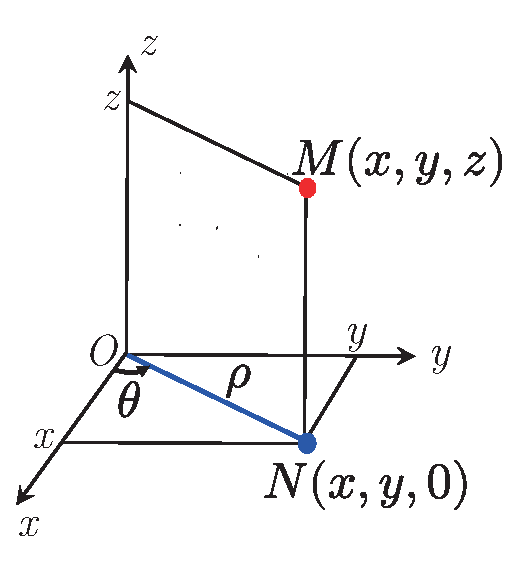
\includegraphics[width=0.85\linewidth]{picture/C-3/柱坐标1.eps}
		\label{柱坐标1}
	\end{minipage}
}
\subfigure[球坐标]{
	\begin{minipage}[b]{0.4\linewidth}
		\centering
		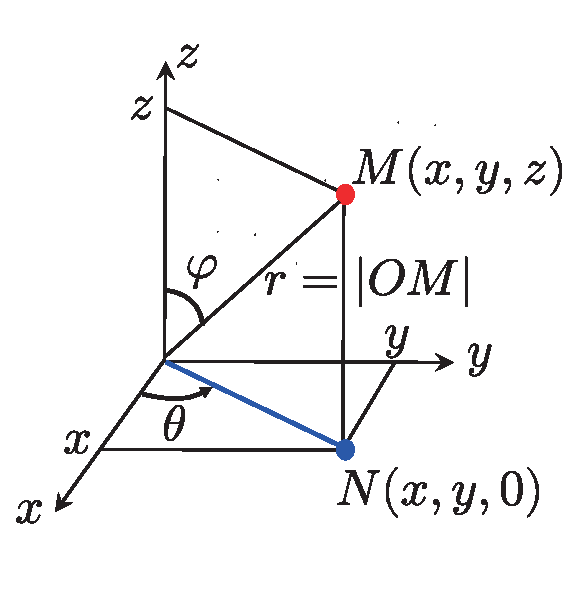
\includegraphics[width=0.9\linewidth]{picture/C-3/球坐标1.eps}
		\label{球坐标1}
	\end{minipage}
}
\caption{球坐标与柱坐标}
\end{center}
\end{figure}

\defination[球坐标]\index{QZB@球坐标}
空间直角坐标系中点$M(x,y,z).$
\begin{enumerate}[(1)]
	\setlength{\itemindent}{3em}
	\setlength{\topsep}{0.01em}
	\setlength{\itemsep}{0.01em}
	\item 它在$xOy$面上的投影点$N(x,y,0)$;
	\item 用$r$表示点$M$到原点$O$的距离;
	\item 用$\varphi $表示$\overrightarrow{OM}$到$z$轴正向的夹角;
	\item 用$\theta $表示从$x$轴正向到原点$\overrightarrow{ON}$的转角.
\end{enumerate}
\par 那么我们称三元有序数组$(r ,\varphi ,\theta )$为点$M$的{\color{dy}球坐标}.如图\ref{球坐标1}.
\begin{enumerate}[]
	\setlength{\topsep}{0.01em}
	\setlength{\itemsep}{0.01em}
	\item {\color{dy}球坐标与直角坐标的关系}
	\begin{equation}
	\begin{cases}
	x=r\sin \varphi  \cos\theta,\\
	y=r\sin \varphi  \sin\theta ,\\
	z=r\cos \varphi.
	\end{cases}
	\quad 
	\begin{array}{l}
	0 \le r < +\infty\\ 
	0 \le \theta \le 2\pi \quad \mbox{或} \quad -\pi \le \theta \le \pi \\ 
	0 \le \varphi \le \pi\\ 
	\end{array} 
	\end{equation}
	\item {\color{dy}球坐标的坐标曲面}
	\begin{enumerate}[]
		\setlength{\itemindent}{1em}
		\setlength{\topsep}{0.01em}
		\setlength{\itemsep}{0.01em}
		\item $r = r_0 $:以原点为球心,半径为$r_0$的{\color{dy}球面};
		\item $\varphi  =\varphi_0$:顶点在原点$O$,半顶角为$\varphi_0$的{\color{dy}圆锥面};
		\item $\theta =\theta_0$:从$z$轴出发且从$x$轴的转角为$\theta_0$的{\color{dy}半平面};
	\end{enumerate}
	点$M(r_0 ,\varphi_0 ,\theta_0 )$是这三个曲面的交点.
\end{enumerate}

\subsection{曲面的参数方程}
\tdefination[曲面的参数方程]\index{QMDCSFC@曲面的参数方程}
一般地,曲面可以用两个参数的方程表示:
\begin{equation}
\begin{cases}
x=x(u,v),\\
y=y(u,v),\\
z=z(u,v)
\end{cases}
\end{equation}
\par 给定参数$(u,v)$的一组值,就能确定曲面上一个点的位置.
\par 曲面就是这些点的集合:
\begin{equation*}
S=\left\lbrace  \left( x(u,v),y(u,v),z(u,v)\right)|u \in \mathbb{R},v \in \mathbb{R} \right\rbrace \quad \huo \quad  S=\left\lbrace  \left(x(u,v),y(u,v),z(u,v) \right) | (u,v) \in D \right\rbrace 
\end{equation*}
\par 其中,$D$是$\mathbb{R}^2$的一个区域,它是参数$(u,v)$的取值范围.以下给出几个例子:

\example[圆柱面的参数方程]
求圆柱面$x^2+y^2=a^2$的参数方程.\\
解:代入\hyperref[柱坐标]{\color{超链接}柱坐标变换}$\displaystyle \begin{cases}
x=\rho \cos\theta \\
y=\rho \sin\theta \\
z=z
\end{cases}$\\
得到圆柱面的柱坐标方程为$S:\rho =a.$,即圆柱面的参数方程为:
\begin{equation*}
S:\begin{cases}
x=a\cos\theta, \\
y=a\sin\theta,\\
z=z.
\end{cases}
\begin{array}{l}
0 \le \theta \le 2\pi \quad \mbox{或} \quad  -\pi \le \theta \le \pi\\
-\infty < z < +\infty\\
\end{array}
\end{equation*}

\newpage
\example[球面的参数方程]
求球面$x^2+y^2+z^2=a^2$的参数方程.\\
解:代入\hyperref[球坐标]{\color{超链接}球坐标变换}$\displaystyle 	\begin{cases}
x=r\sin \varphi  \cos\theta,\\
y=r\sin \varphi  \sin\theta ,\\
z=r\cos \varphi.
\end{cases}$\\
得到圆柱面的柱坐标方程为$S:r =a.$,即圆柱面的参数方程为:
\begin{equation*}
S:	\begin{cases}
x=a\sin \varphi  \cos\theta,\\
y=a\sin \varphi  \sin\theta ,\\
z=a\cos \varphi.
\end{cases}
\begin{array}{l}
0 \le \theta \le 2\pi \quad \mbox{或} \quad -\pi \le \theta \le \pi \\ 
0 \le \varphi \le \pi\\ 
\end{array} 
\end{equation*}

\section{空间曲线的方程}
\subsection{空间曲线的参数方程}
\tdefination[空间曲线的参数方程]\index{QXDCSFC@曲线的参数方程}
空间曲线可以看作是质点的运动轨迹。曲线$C$上动点$M(x,y,z)$表示为
\begin{equation}
\begin{cases}
x=x(t),\\
y=y(t),\\
z=z(t).
\end{cases}
\, a \le t \le b.
\label{空间曲线的参数方程}
\end{equation}
\par 那么式\ref{空间曲线的参数方程}就称为空间曲线$C$的参数方程,其中$t$为参数.(空间曲线参数方程中参数可取时间 、转动角度或其它变量.)以下举两个例子:

\example[直线的参数方程]
{\color{dy}几何意义}\quad 直线可以看作是做匀速直线运动的质点的几何轨迹(速度:$\overrightarrow{v}=(m,n,t)$,时间:$t$).
\par{\color{dy} 参数方程}\quad $\displaystyle L:\begin{cases}
x=x_0+mt,\\
y=y_0+nt,\\
z=z_0+pt.
\end{cases}\, -\infty  < t < +\infty $

\newpage
\example[圆柱螺旋线的参数方程]\index{YZRXX@圆柱螺旋线}
{\color{dy}几何意义}\quad 动点$M$在圆柱面$S:x^2+y^2=R^2$上以等角速度$\omega $绕$z$轴旋转,同时又以线速度$v$沿平行于$z$轴的正向均匀地上升.
\par {\color{dy}参数方程}\quad $\displaystyle L:\begin{cases}
x=R\cos \omega t,\\
y=R\sin \omega t,\\
z=vt.
\end{cases}$
令$\displaystyle \theta =\omega t,b=\frac{v}{\omega}$得:
$\displaystyle L:\begin{cases}
x=R\cos \theta ,\\
y=R\sin \theta,\\
z=b\theta .
\end{cases}\, -\infty  < \theta  < +\infty $

\subsection{空间曲线的一般方程}
\tdefination[空间曲线的一般方程]\index{QXDYBFC@曲线的一般方程}
空间曲线可以看作是两曲面的交线。即
\begin{equation}
C:
\begin{cases}
F(x,y,z)=0,\\
G(x,y,z)=0.
\end{cases}
\end{equation}
{\color{dy}空间曲线一般方程的特点}
\begin{enumerate}[1.]
	\setlength{\itemindent}{2em}
	\setlength{\topsep}{0.01em}
	\setlength{\itemsep}{0.01em}
	\item 空间曲线的一般方程不唯一:可以用任意两个过$C$的曲面$S_1,S_2$的方程联立得到的方程组来表示;
	\item 空间曲线$C$位于曲面$S_1,S_2$方程的线性组合确定的曲面$\Sigma $上:
	\begin{equation}
	\Sigma :\lambda F(x,y,z)+\mu G(x,y,z)=0.\quad (\lambda ,\mu \in \mathbb{R},\lambda^2+\mu^2 \ne 0)
	\end{equation}
\end{enumerate}

\example[空间曲线举例]
方程组$\displaystyle 
\begin{cases}
x^2+y^2+z^2-2Rz=0,\\
x^2+y^2+z^2-R^2=0.
\end{cases}$
表示怎样的曲线?
\begin{enumerate}[1.]
	\setlength{\itemindent}{2em}
	\setlength{\topsep}{0.01em}
	\setlength{\itemsep}{0.01em}
	\item {\color{dy}直接分析}
	\begin{enumerate}[]
		\setlength{\itemindent}{2em}
		\setlength{\topsep}{0.01em}
		\setlength{\itemsep}{0.01em}
		\item $x^2+y^2+z^2-2Rz=0$表示圆心为$(0,0,R)$半径为$R$的球面;
		\item $x^2+y^2+z^2-R^2=0$表示圆心为$(0,0,0)$半径为$R$的球面.
	\end{enumerate}
	即该曲线可以表示为两个球面的交线。
	\item {\color{dy}变形方程后分析 
		$\displaystyle 
		\begin{cases}
		x^2+y^2+z^2=R^2,\\
		z=\displaystyle \frac{1}{2}R.
		\end{cases}$}
	\begin{enumerate}[]
		\setlength{\itemindent}{2em}
		\setlength{\topsep}{0.01em}
		\setlength{\itemsep}{0.01em}
		\item $x^2+y^2+z^2=R^2$表示圆心为$(0,0,R)$半径为$R$的球面;
		\item $z=\displaystyle  \frac{1}{2}R$表示平面.
	\end{enumerate}
	即该曲线也可以表示为球面和平面的交线。
	\item {\color{dy}变形方程后分析 
		$\displaystyle 
		\begin{cases}
		x^2+y^2=\displaystyle \frac{3}{4} R^2,\\
		z=\displaystyle \frac{1}{2}R.
		\end{cases}$}
	\begin{enumerate}[]
		\setlength{\itemindent}{2em}
		\setlength{\topsep}{0.01em}
		\setlength{\itemsep}{0.01em}
		\item $x^2+y^2=\displaystyle \frac{3}{4} R^2$表示对称轴为$z$轴的圆柱面;
		\item $z=\displaystyle  \frac{1}{2}R$表示平面.
	\end{enumerate}
	即该曲线还可以表示为圆柱面和平面的交线。
\end{enumerate}

\example[维维安尼(Viviani)曲线]\index{Viviani@Viviani(维维安尼曲线)}
方程组
\begin{equation*}
\begin{cases}
x^2+y^2+z^2=a^2,\\
x^2+y^2=ax.
\end{cases}
\quad (a>0)
\end{equation*}
\par 的图像是球面$x^2+y^2+z^2=a^2$与母线平行于$z$轴的圆柱面$\displaystyle (x-\frac{a}{2})^2+y^2=\frac{a^2}{4}$的交线,称为{\color{dy}维维安尼(Viviani)曲线},也可以用等价的方程组
\begin{equation*}
\begin{cases}
z^2+ax=a^2,\\
x^2+y^2=ax.
\end{cases}
\quad (a>0)
\end{equation*}
\par 来表示,其中$0 \le x \le a$.
\jg
\subsection{空间圆}\index{KJY@空间圆}
\tdefination[空间圆周]
一般地,一个球面
$$
S:(x-x_0)^2+(y-y_0)^2+(z-z_0)^2=R^2
$$
\par 被平面
$$\pi:Ax+By+Cz+D=0$$
\par 截下一个{\color{dy}空间圆周}\index{KJYZ@空间圆周},当且仅当球心$M_0(x_0,y_0,z_0)$到平面$\pi $的距离$d$小于等于球面半径$R$,即
\begin{equation}
d=\frac{|Ax_0+By_0+Cz_0+D|}{\sqrt{A^2+B^2+C^2}} \le R.
\end{equation}

\theorem[空间圆的圆心和半径]
记圆周上任意一点的矢径为:$\overrightarrow{r}=(x,y,z)$圆周的圆心的矢径为:$\overrightarrow{r_0}=(x_0,y_0,z_0)$,则球面的向量式和\hyperref[平面的向量式法式方程]{\color{超链接}平面的向量式法式方程}分别为:
\begin{equation*}
\begin{array}{l}
S:(\overrightarrow{r}-\overrightarrow{r_0})\cdot (\overrightarrow{r}-\overrightarrow{r_0})=R^2\\
\pi : \overrightarrow{n_0} \cdot \overrightarrow{r}-p=0\quad (|\overrightarrow{n_0}=1|)
\end{array}
\end{equation*}

\begin{enumerate}[]
	\setlength{\itemindent}{2em}
	\setlength{\topsep}{0.01em}
	\setlength{\itemsep}{0.01em}
	\item {\color{dy}原理} \quad 空间圆轴$C$的圆心就是过球心且垂直于$\pi$的直线与$\pi $的交点.
	\item {\color{dy}表达式} \jg \quad
	$
	\begin{cases}
	\overrightarrow{r}=\overrightarrow{r_0}+t\overrightarrow{n},\\
	\overrightarrow{n_0} \cdot \overrightarrow{r}-p=0.
	\end{cases}
	\Longleftrightarrow \, \overrightarrow{r_0}+(p-\overrightarrow{n_0}\cdot \overrightarrow{r_0})\overrightarrow{n_0}.
	$\\
	\jg \hspace*{6em}球心到圆心的距离为
	$
	d=|p-\overrightarrow{n} \cdot \overrightarrow{r_0}| \le R.
	$\\
	\jg 综上,{\color{dy}圆心的矢径}为:$\overrightarrow{r_0}+(p-\overrightarrow{n_0}\cdot \overrightarrow{r_0})\overrightarrow{n_0}$.\\
	\jg  {\color{dy}空间圆的半径}为:$r=\sqrt{R^2-d^2}=\sqrt{R^2-(p-\overrightarrow{n} \cdot \overrightarrow{r_0})^2}$
\end{enumerate}

\section{柱面}
\subsection{柱面的定义}
\tdefination[柱面]
在空间中,由平行于定方向且与一条定曲线相交的一族平行直线所构成的曲面叫做{\color{dy}柱面}\index{ZM1@柱面!ZM@柱面}.
\par 从几何上看,柱面就是由一条平行于直线 $L$ 的直线沿曲线 $C$ 连续平移而形成的{\color{dy}平行直线族}.\index{PXZSC@平行直线族}\\
其中,
\sj
\begin{enumerate}[]
	\setlength{\itemindent}{2em}
	\setlength{\topsep}{0.01em}
	\setlength{\itemsep}{0.01em}
	\item 动直线$L$ 叫做柱面的{\color{dy}直母线}\index{ZM1@柱面!ZMX@直母线},
	\item 定曲线$C$叫做柱面的{\color{dy}准线}\index{ZM1@柱面!ZX@准线},
	\item 平行于动直线的方向$\overrightarrow{v}$叫做{\color{dy}直母线方向}\index{ZM1@柱面!ZMXFX@直母线方向}.
\end{enumerate}
注意:柱面的准线不是唯一的,与每一条母线都相交的曲线都可以作为柱面的准线.

\subsection{柱面方程}
\ttheorem[柱面的一般方程]\index{ZM1@柱面!ZMDYBFC@柱面的一般方程}

\par {\color{dy}已知}:准线$C:
\begin{cases}
F(x,y,z)=0,\\
G(x,y,z)=0
\end{cases}$
和母线的方向向量$\overrightarrow{v}=(m,n,p)$\\
\par {\color{dy}原理}:在柱面上取动点$M(x,y,z)$,作平行于母线的方向$\overrightarrow{v}$的直线交准线$C$于点$N(u,v,w).$由\hyperref[点向式方程]{\color{超链接}直线的点向式方程}(平行向量的条件)和点在曲面上可以得到。
\par {\color{dy}表达式}:
\begin{equation}
\begin{cases}
\displaystyle \frac{x-u}{m}=\frac{y-v}{n}=\frac{z-w}{p}=t,\\
F(u,v,w)=0.\\
G(u,v,w)=0.\\
\end{cases}
\Longrightarrow \quad 
S:
\begin{cases}
F(x-mt,y-nt,z-pt)=0.\\
G(x-mt,y-nt,z-pt)=0.
\end{cases}
\end{equation}
\par 消去参数$t$可以得到柱面的一般方程。

\theorem[柱面的参数方程]\index{ZM1@柱面!ZMDCSFC@柱面的参数方程}

\par {\color{dy}已知}:准线$C:
\begin{cases}
x=u(t),\\
y=v(t),\\
z=w(t).
\end{cases}$
和母线的方向向量$\overrightarrow{v}=(m,n,p)$\\
\par {\color{dy}原理}:在柱面上取动点$M(x,y,z)$,作平行于母线的方向$\overrightarrow{v}$的直线交准线$C$于点$N(u(t),v(t),w(t)).$由\hyperref[直线的参数方程]{\color{超链接}直线的参数方程}可以得到。
\par {\color{dy}表达式}:
\begin{equation}
S:\begin{cases}
x=u(t)+ms,\\
y=v(t)+ns,\\
z=w(t)+ps.
\end{cases}
\quad (-\infty<t,s<+\infty)
\end{equation}

\example[特殊的柱面方程]

\par  一般地,方程$F(x,y)=0$在$Oxyz$空间表示柱面$S$,在$xOz$平面表示曲线$C$.
\par {\color{dy}方程特点}:方程中不含变量$z$.
\par {\color{dy}几何特点}:柱面$S$上点$M(x,y,z)$在$xOy$面上的投影点$N(x,y,0)$在曲面$C$上.\\
\hspace*{7em}柱面的母线平行于$z$轴.\\
\hspace*{7em}柱面的准线为$xOy$平面上的曲线$C$.
\par 总结如下
\begin{center}
\begin{tabular}{|c|c|c|}
	\hline
	方程 &母线   &  准线    \\
	\hline
	 \hspace*{1em} $F(x,y)=0$ \hspace*{1em} &\hspace*{1em} 平行于$z$轴  \hspace*{1em}  & \hspace*{1em}  在$xOy$平面上的曲线
	$C:
	\begin{cases}
	F(x,y)=0,\\
	z=0
	\end{cases}
	$ \hspace*{1em}  \\
	\hline
\hspace*{1em} $G(y,z)=0$ \hspace*{1em}  &\hspace*{1em} 平行于$x$轴  \hspace*{1em}  & \hspace*{1em}  在$yOz$平面上的曲线
$C:
\begin{cases}
G(y,z)=0,\\
x=0
\end{cases}
$  \hspace*{1em}  \\
	\hline
\hspace*{1em} $H(x,z)=0$ \hspace*{1em} &\hspace*{1em} 平行于$y$轴  \hspace*{1em}  & \hspace*{1em} 在$zOx$平面上的曲线
$C:
\begin{cases}
H(x,z)=0,\\
y=0
\end{cases}
$\hspace*{1em} \\
	\hline
\end{tabular}
\end{center}

\section{锥面} 
\subsection{锥面的定义}
\tdefination[锥面]\index{ZM2@锥面!ZM2@锥面}
\par 在空间中,由曲线$C$上的点与不在 $C$ 上的一个定点 $M_0$ 的连线组成的曲面称为{\color{dy}锥面} .
\par 从几何上看,锥面就是由过同一定点 $M_0$的动直线 $L$沿曲线 $C$连续滑动而形成的{\color{dy}相交直线族}.\\
其中,
\sj
\begin{enumerate}[]
	\setlength{\itemindent}{2em}
	\setlength{\topsep}{0.01em}
	\setlength{\itemsep}{0.01em}
	\item 定点$M_0$ 叫做锥面的{\color{dy}顶点}\index{ZM2@锥面!DD@顶点},
	\item 动直线$L$ 叫做锥面的{\color{dy}直母线}\index{ZM2@锥面!ZMX@直母线},
	\item 定曲线$C$叫做锥面的{\color{dy}准线}\index{ZM2@锥面!ZX@准线}.
\end{enumerate}
注意:锥面的准线不是唯一的,与每一条母线都相交的曲线都可以作为锥面的准线.

\subsection{一般锥面的方程}

\ttheorem[锥面的一般方程]\index{ZM2@锥面!ZMDYBFC@锥面的一般方程}

\par {\color{dy}已知}:锥面的顶点$M_0(x_0,y_0,z_0)$,准线$C:
\begin{cases}
F(x,y,z)=0,\\
G(x,y,z)=0.
\end{cases}$
\par {\color{dy}原理}:连接点$M_0,M$的直线交曲线$C$于点$N(u,v,w)$,由\hyperref[两点式方程]{\color{超链接}直线的两点式方程}在及点在曲线上可以得到,即
\begin{equation*}
\begin{cases}
\displaystyle \frac{u-x_0}{x-x_0}=\frac{v-y_0}{y-y_0}=\frac{w-z_0}{z-z_0}=t,\\
F(u,v,w)=0,\\
G(u,v,w)=0.
\end{cases}
\end{equation*}
\par {\color{dy}表达式}:
\begin{equation}
	S:
	\begin{cases}
	F(x_0+(x-x_0)t,y_0+(y-y_0)t,z_0+(z-z_0)t)=0,\\
	G(x_0+(x-x_0)t,y_0+(y-y_0)t,z_0+(z-z_0)t)=0.
	\end{cases}
\end{equation}

\theorem[锥面的参数方程]\index{ZM2@锥面!ZMDCSFC@锥面的参数方程}

\par {\color{dy}已知}:锥面的顶点$M_0(x_0,y_0,z_0)$,准线$C:
\begin{cases}
x=u(t),\\
y=v(t),\\
z=w(t).
\end{cases}$
\par {\color{dy}原理}:连接点$M_0,M$的直线交曲线$C$于点$N(u(t),v(t),w(t))$,由\hyperref[两点式方程]{\color{超链接}直线的两点式方程}和\hyperref[直线的参数方程]{\color{超链接}直线的参数方程}及点在曲线上可以得到,即
\begin{equation*}
\displaystyle \frac{u(t)-x_0}{x-x_0}=\frac{v(t)-y_0}{y-y_0}=\frac{w(t)-z_0}{z-z_0}=t.\\
\end{equation*}
\par {\color{dy}表达式}:
\begin{equation}
S:
\begin{cases}
x=x_0+(u(t)-x_0)s,\\
y=y_0+(v(t)-y_0)s,\\
z=z_0+(w(t)-z_0)s.
\end{cases}
\quad (-\infty <t,s<+\infty )
\end{equation}

\example[特殊的锥面方程]
\begin{table}[h]
\begin{center}
\begin{tabular}{|c|c|}
	\hline
	名称 &方程 \\
	\hline
	  \hspace*{1em} $S:z^2=(x^2+y^2)$ \hspace*{1em} & 圆锥面(夹角为$90^{\circ}$)  \\
	\hline
\hspace*{1em} $S:xy+yz+zx=0$ \hspace*{1em}   & 圆锥面 \\
	\hline
\multirow{2}{*}{\hspace*{1em} $\displaystyle S:\frac{x^2}{a^2}+\frac{y^2}{b^2}-\frac{z^2}{c^2}=0$ \hspace*{1em}}  &\multirow{2}{*}{椭圆锥面(渐进锥面)}   \\
	& \\
	\hline
\end{tabular}
	\caption{特殊的锥面方程}
	\label{特殊的锥面方程}
\end{center}
\end{table}
\sj
\subsection{锥面方程的特点}
\tdefination[齐次方程]
如果对于任意非零实数$t$,函数$F(x,y,z)$满足
\begin{equation}
F(tx,ty,tz)=t^nF(x,y,z)
\end{equation}
其中,$n$为整数.则称函数$F(x,y,z)$为关于$x,y,z$的{\color{dy}$\, \,  n$次齐次函数}.\index{QCHS@齐次函数}
\par 方程$F(x,y,z)=0$为关于$x,y,z$的{\color{dy}$\, \,  n$次齐次方程}.\index{QCFC@齐次方程}
	\par 观察表\ref{特殊的锥面方程}可以发现方程中每一项都是二次的,称为二次齐次方程.令$F(x,y,z=xy+yz+zx)$,则有二次齐次函数:
	$$
	F(tx,ty,tz)=t^2F(x,y,z)
	$$
	
	\theorem[原点为顶点的锥面方程的特点]
	以坐标原点为顶点的锥面方程$\Longleftrightarrow$ $x, y, z$的齐次方程 .\\
原理:利用$F(tx,ty,tz)=t^nF(x,y,z)=0 \Longleftrightarrow  F(tx,ty,tz)=F(x,y,z)=0$
\\$ \Longleftrightarrow$若点$M$在曲面上,则由原点$O$和点$M$所确定的直线也在曲面上.\colorbox{文字底色}{(解析语言$\Longleftrightarrow$几何语言)}

	\addinference[一般锥面方程的特点]
以点$M_0(x_0,y_0,z_0)$为顶点的锥面方程$\Longleftrightarrow$ $(x-x_0), (y-y_0), (z-z_0)$的齐次方程 .\\

\section{旋转曲面}\label{旋转曲面}
\subsection{旋转曲面的定义}
\tdefination[旋转曲面]
一条空间曲线$C$绕一条定直线$L$旋转一周所得到的曲面$S$称为{\color{dy}旋转曲面}\index{XZQM@旋转曲面}.
\\其中,
\begin{enumerate}[]
	\setlength{\itemindent}{2em}
	\setlength{\topsep}{0.01em}
	\setlength{\itemsep}{0.01em}
	\item 定直线$L$称为旋转曲面的{\color{dy}旋转轴}.\index{XZQM@旋转曲面!XZZ@旋转轴}
	\item 曲线$C$称为旋转曲面的{\color{dy}母线}.\index{XZQM@旋转曲面!MX@母线}
	\item 母线$C$上每个点$M_0$绕旋转轴 $L$旋转得到一个圆,称为{\color{dy}纬圆}.\index{XZQM@旋转曲面!WY@纬圆}(纬圆与轴垂直)
	\item 过旋转轴$L$的半平面与旋转面$S$ 的交线称为{\color{dy}经线}\index{XZQM@旋转曲面!JX@经线}({\color{dy}子午线}\index{XZQM@旋转曲面!ZWX@子午线}).(经线可以作为母线,但母线未必是经线.)
\end{enumerate}

\subsection{旋转曲面的方程}
\ttheorem[特殊情况的旋转曲面方程]
母线为$yOz$面上的曲线 $C:f(y,z)= 0$ ,旋转轴为$z$轴 .在旋转曲面$S$上取动点$M(x,y,z)$,过点$M$作纬圆交母线$C$于点$N(x_0,y_0,z_0)$.则
\begin{equation*}
S:
\begin{cases}
x_0=0\\
z_0=z\\
\sqrt{x^2+y^2}=|y_0|
\end{cases}
\Longrightarrow
\begin{cases}
y_0=\pm \sqrt{x^2+y^2}\\
z_0=z
\end{cases}
\end{equation*}
将上式代入$f(y_0,z_0)$得:$S:f(\pm \sqrt{x^2+y^2},z)=0$,类似地,我们可以得到
\begin{table}[h]
	\begin{center}
		\begin{tabular}{|c|c|c|}
			\hline
			母线&旋转轴  &旋转曲面方程  \\
			\hline
			\multirow{2}{*}{\hspace*{1cm}$yOz$面上的曲线$C:f(y,z)=0$} \hspace*{1cm}& $z$轴 & \hspace*{1cm}$S:f(\pm  \sqrt{x^2+y^2},z)=0$  \hspace*{1cm}\\
			\cline{2-3}
			&$y$轴   & \hspace*{1cm}$S:f(y,\pm  \sqrt{x^2+z^2})=0$ \hspace*{1cm}\\
			\hline
			\multirow{2}{*}{\hspace*{1cm}$xOz$面上的曲线$C:f(x,z)=0$\hspace*{1cm}} & $z$轴 &  \hspace*{1cm} $S:f(\pm  \sqrt{x^2+y^2},z)=0$ \hspace*{1cm}\\
			\cline{2-3}
			& $x$轴 &\hspace*{1cm} $S:f(x,\pm  \sqrt{y^2+z^2})=0$  \hspace*{1cm} \\
			\hline
			\multirow{2}{*}{\hspace*{1cm}$xOy$面上的曲线$C:f(x,y)=0$\hspace*{1cm}} & $y$轴 &  \hspace*{1cm} $S:f(\pm  \sqrt{x^2+z^2},y)=0$ \hspace*{1cm}\\
			\cline{2-3}
			& $x$轴 & \hspace*{1cm} $S:f(x,\pm  \sqrt{y^2+z^2})=0$  \hspace*{1cm} \\
			\hline
		\end{tabular}
\end{center}
\caption{母线在坐标平面内、旋转轴为坐标轴的旋转曲面方程}
\label{特殊情况的旋转曲面方程}
\end{table}

\ttheorem[旋转曲面的一般方程]\index{XZQM@旋转曲面!XZQMDYBFC@旋转曲面的一般方程}
\par {\color{dy}已知}:在旋转曲面$S$上取动点$M(x,y,z)$,过点$M$作垂直于旋转轴$L=(m,n,t)$的平面$\pi $,交轴$L$于点$Q$,交母线$
C:
\begin{cases}
	F(x,y,z)=0\\
	G(x,y,z)=0
\end{cases}
$于点$N(u,v,w)$,取轴上一定点$M_0(x_0,y_0,z_0)$.\\
(即需知道{\color{dl}1. 旋转轴上一点};{\color{dl}2. 旋转轴的方向向量};{\color{dl}3. 母线方程})
\par {\color{dy}原理}:旋转曲面的定义
\begin{equation*}
\begin{cases}
\mbox{点}N\mbox{在母线上}\\
\mbox{平面与轴垂直}\\
\mbox{轴上一点到垂直与轴的纬圆上任意一点的距离始终相等}
\end{cases}
\,\, \Longleftrightarrow \, \,
\begin{cases}
N \in C \\
\overrightarrow{NM}  \, \bot \,  \overrightarrow{v}\\
|M_0M|=|M_0N|
\end{cases}
\end{equation*}
\par {\color{dy}表达式}:
\begin{equation}
S:
	\begin{cases}
	F(u,v,w)=0,\\
	G(u,v,w)=0,\\
	m(x-u)+n(y-v)+t(z-w)=0,\\
	(x-x_0)^2+(y-y_0)^2+(z-z_0)^2=(u-x_0)^2+(v-y_0)^2+(z-z_0)^2
	\end{cases}
\end{equation}
消去参数$u,v,w$即可得到旋转曲面的一般方程.

\newpage

\theorem[旋转曲面的参数方程]\index{XZQM@旋转曲面!XZQMDCSFC@旋转曲面的参数方程}
空间曲线
$$\Gamma:
\begin{cases}
x=x(t),\\
y=y(t),\\
z=z(t)\\
\end{cases}
\quad 
\alpha \le t \le \beta
$$
绕$z$轴选择所得到的旋转曲面$S$的方程.
\par {\color{dy}已知}:在旋转曲面$S$上取动点$M(x,y,z)$,过点$M$作纬圆$C$位于平面$\pi :z=z(t)$上,设其圆心为点$Q$,半径为$r(t)$
\par {\color{dy}原理}:$r(t)=\sqrt{x^2(t)+y^2(t)}.$,类似于\hyperref[柱坐标]{\color{超链接}柱坐标变换},先定$t$求出每一个$t$对应的纬圆方程,再让$t$在定义的范围内摆动(即一个个连续的纬圆形成一个曲面).
\par {\color{dy}表达式}:
\begin{equation}
S:
\begin{cases}
x=\sqrt{x^2(t)+y^2(t)}\, \cos \theta,\\
y=\sqrt{x^2(t)+y^2(t)}\, \sin \theta,\\
z=z(t)
\end{cases}
\quad 
\theta \in [0,2\pi],\,
\alpha \le t \le \beta
\end{equation}

\section{常见的二次曲面}
\subsection{二次曲面的定义}
\tdefination[二次曲面]\index{ECQM@二次曲面}
三元二次方程
\begin{equation}
a_1 x^2 + a_2 y^2 + a_3 z^2 +b_1 xy +b_2 yz+b_3 zx + c_1x+c_2y+c_3z+d=0
\end{equation}
所确定的曲面称为{\color{dy}二次曲面},其中二次项系数不全为$0$.

\jg
\subsection{二次曲面的基本类型}

\begin{enumerate}
	\setlength{\itemindent}{0em}
	\setlength{\topsep}{0.01em}
	\setlength{\itemsep}{0.01em}
	\item  \link[旋转曲面]:\link[球面]、\link[旋转椭球面]、\link[圆柱面]、\link[圆锥面]、\link[旋转椭球面]、\link[旋转单叶双曲面]、\link[旋转双叶双曲面]、\link[旋转抛物面].(注:圆环面不是二次曲面)
	\item  \link[椭球面]、\link[双曲面]、\link[抛物面]、\link[二次锥面]和\link[二次柱面].
\end{enumerate}

\newpage
\subsection{二次曲面的性质}
对称性
\begin{table}[!h]
	\begin{minipage}[!h]{\columnwidth}
		\centering
		\begin{tabular}{|c|c|}
				\hline
			\kg 方程条件\kg & \kg  曲面对称性 \kg\\
			\hline
			\kg $F(x,y,z)=F(x,y,-z)$\kg & \kg 关于$xOy$面对称\kg \\
			\hline
			\kg $F(x,y,z)=F(-x,y,z)$ \kg & \kg 关于$yOz$面对称\kg \\
			\hline
			\kg $F(x,y,z)=F(x,-y,z)$ \kg & \kg 关于$zOx$面对称\kg \\
			\hline
		\end{tabular}
	\caption{二次曲面关于面的对称性}
	\label{二次曲面关于面的对称性}
	\end{minipage}
	\\[12pt]%设置两个表格之间的空白行距离
	\begin{minipage}[h]{\columnwidth}
		\centering
		\begin{tabular}{|c|c|}
			\hline
			\kg 方程条件 \kg &  \kg  曲面对称性 \kg\\
			\hline
			\kg $F(x,y,z)=F(x,-y,-z)$ \kg & \kg 关于$x$轴对称 \kg \\
			\hline
			\kg $F(x,y,z)=F(-x,y,-z)$\kg & \kg 关于$y$轴对称 \kg  \\
			\hline
			\kg $F(x,y,z)=F(-x,-y,z)$ \kg & \kg 关于$z$轴对称 \kg \\
			\hline
		\end{tabular}
	\caption{二次曲面关于轴的对称性}
	\label{二次曲面关于轴的对称性}
	\end{minipage}
	\\[12pt]%设置两个表格之间的空白行距离
\begin{minipage}[h]{\columnwidth}
	\centering
	\begin{tabular}{|c|c|}
		\hline
		\kg 方程条件 \kg & \kg  曲面对称性 \kg \\
		\hline
		\kg $F(x,y,z)=F(-x,-y,-z)$ \kg & \kg 关于原点对称 \kg \\
		\hline
	\end{tabular}
	\caption{二次曲面关于原点的对称性}
	\label{二次曲面关于原点的对称性}
\end{minipage}
	\vspace{-0.1cm}%设置第二个表格与正文下文的空白行距离
\end{table}

\subsection{椭球面}\index{TQM@椭球面}\label{椭球面}
\sja
\begin{enumerate}
	\setlength{\itemindent}{0em}
	\setlength{\topsep}{0.01em}
	\setlength{\itemsep}{0.01em}
	\item 椭球面的基本定义与基本方程
\jg

\enbelowdefination[椭球面]
\hspace*{1em} 方程$\displaystyle S:\frac{x^2}{a^2}+\frac{y^2}{b^2}+\frac{z^2}{c^2}=1$所表示的曲面称为中心在原点的{\color{dy}椭球面}.该方程称为{\color{dy}椭球面的标准方程}\index{TQM@椭球面!TQMDBZFC@椭球面的标准方程}.其中$a,b,c$为正的常数,称为椭球面的{\color{dy}半轴}\index{TQM@椭球面!BZ@半轴}.
\par {\color{dy}特殊情况}
\sja
\begin{enumerate}
	\setlength{\itemindent}{1em}
	\setlength{\topsep}{0.01em}
	\setlength{\itemsep}{0.01em}
	\item 当$a=b=c$时,表示球面:$S:x^2+y^2+z^2=a^2$.
	\item 当$a=b$时表示{\color{dy}旋转椭球面}\index{TQM@椭球面!XZTQM@旋转椭球面}\label{旋转椭球面}:$ \displaystyle S:\frac{x^2+y^2}{a^2}+\frac{z^2}{c^2}=1$.
\end{enumerate}

\enbelowtheorem[椭球面的一般方程]
\hspace*{1em} 方程
\begin{equation}
\Sigma : \frac{(x-x_0)^2}{a^2}+\frac{(y-y_0)^2}{b^2}+\frac{(z-z_0)^2}{c^2}=1
\end{equation}
所表示的曲面称为中心在点$(x_o,y_0,z_0)$的{\color{dy}椭球面}.该方程称为{\color{dy}椭球面的一般方程}\index{TQM@椭球面!TQMDBZFC@椭球面的一般方程}其中$a,b,c$为正的常数,称为椭球面的{\color{dy}半轴}.

\item 椭球面$\displaystyle S:\frac{x^2}{a^2}+\frac{y^2}{b^2}+\frac{z^2}{c^2}=1$的几何性质
\begin{enumerate}
	\setlength{\topsep}{0.01em}
	\setlength{\itemsep}{0.01em}
	\item 对称性\\
	\kg \kg 由表$\,$\ref{二次曲面关于面的对称性}  $-$ \ref{二次曲面关于原点的对称性}$\,$可知椭球面关于各坐标面、坐标轴及原点都对称 .
	
	\item 有界性\\
	\kg \kg 椭球面上的点$(x,y,z)$满足:
	\begin{equation*}
	\begin{cases}
	\displaystyle  \frac{x^2}{a^2}\le 1,\\
	\displaystyle  \frac{y^2}{b^2} \le 1,\\
	\displaystyle  \frac{z^2}{c^2} \le 1. 
	\end{cases}
\quad \Longleftrightarrow \quad
	\begin{cases}
	|x| \le a,\\
	|y| \le b,\\
	|z| \le c.
	\end{cases}
	\end{equation*}
	$\Longleftrightarrow$椭圆包含在由六个平面$x=\pm a,y=\pm b,z=\pm c$所围成的长方体.
\end{enumerate}

\item  椭球面$\displaystyle S:\frac{x^2}{a^2}+\frac{y^2}{b^2}+\frac{z^2}{c^2}=1$的平截线
\jg

\enbelowdefination[平截线]
\kg 平行于坐标面的平面截曲面的截痕线称作{\color{dy}平截线}\index{PJX@平截线}.
\begin{enumerate}
	\setlength{\itemindent}{1em}
	\setlength{\topsep}{0.01em}
	\setlength{\itemsep}{0.01em}
	\item 截平面:与$xOy$平行的平面$ z = h $ \\ 
	\kg 平截线方程:
	\begin{equation*}
	\begin{cases}
	\displaystyle \frac{x^2}{a^2} + \frac{y^2}{b^2}=1- \frac{h^2}{c^2}\\
	x=h \, (|h|<c)
	\end{cases}
	\quad \Longrightarrow \quad 
	\begin{cases}
	\displaystyle \frac{x^2}{\frac{a^2(c^2-h^2)}{c^2}} + \frac{y^2}{\frac{b^2(c^2-h^2)}{c^2}}=1\\
	x=h \, (|h|<c)
	\end{cases}
	\end{equation*}
	 \kg 平截线图形:中心点在$z$轴,半轴分别为$\displaystyle \frac{a}{c}\sqrt{c^2-h^2},\frac{b}{c}\sqrt{c^2-h^2}$的椭圆
	
	\item 截平面:与$yOz$平行的平面$ x = m $\\
	\kg 平截线方程:
	\begin{equation*}
	\begin{cases}
	\displaystyle \frac{y^2}{b^2} + \frac{z^2}{c^2}=1- \frac{m^2}{a^2}\\
	x=m\,(|m|<a)
	\end{cases}
	\quad \Longrightarrow \quad 
	\begin{cases}
	\displaystyle \frac{y^2}{\frac{b^2(a^2-m^2)}{m^2}} + \frac{z^2}{\frac{c^2(a^2-m^2)}{m^2}}=1\\
	x=m \, (|m|<a)
	\end{cases}
	\end{equation*}
	\kg 平截线图形:中心点在$x$轴,半轴分别为$\displaystyle \frac{b}{a}\sqrt{a^2-m^2},\frac{c}{a}\sqrt{a^2-m^2}$的椭圆
	
	\item 截平面:与$zOx$平行的平面$ y = k $\\
	\kg 平截线方程:
	\begin{equation*}
	\begin{cases}
	\displaystyle \frac{x^2}{a^2} + \frac{z^2}{c^2}=1- \frac{k^2}{b^2}\\
	y=k \, (|k|<b)
	\end{cases}
	\quad \Longrightarrow \quad 
		\begin{cases}
	\displaystyle \frac{x^2}{\frac{a^2(b^2-k^2)}{b^2}} + \frac{z^2}{\frac{c^2(b^2-k^2)}{b^2}}=1\\
	y=k \, (|k|<b)
	\end{cases}
	\end{equation*}
	\kg 平截线图形:中心点在$y$轴,半轴分别为$\displaystyle \frac{a}{b}\sqrt{b^2-k^2},\frac{c}{b}\sqrt{b^2-k^2}$的椭圆
\end{enumerate}

\end{enumerate}

\subsection{双曲面}\index{SQM@双曲面}\label{双曲面}
\sja
\begin{enumerate}
	\setlength{\itemindent}{0em}
	\setlength{\topsep}{0.01em}
	\setlength{\itemsep}{0.01em}
	\item 单叶双曲面的基本定义与基本方程
	\vspace*{0.5em}
	
\enbelowdefination[单叶双曲面]\index{SQM@双曲面!DYSQX@单叶双曲面}
\kg 方程$\displaystyle S:\frac{x^2}{a^2}+\frac{y^2}{b^2}-\frac{z^2}{c^2}=1$表示的曲面称为中心在原点的{\color{dy}单叶双曲面}.该方程称为{\color{dy}单叶双曲面的标准方程}\index{SQM@双曲面!DYSQXDBZFC@单叶双曲面的标准方程}.其中$a,b,c$为正的常数,称为单叶双曲面的{\color{dy}半轴}.
\par {\color{dy}特殊情况}
\kg 当$a=b$时表示{\color{dy}旋转单叶双曲面}\label{旋转单叶双曲面}$\displaystyle S:\frac{x^2+y^2}{a^2}-\frac{z^2}{c^2}=1.$

	\item 单叶双曲面的几何性质
	\sja
	\begin{enumerate}
		\setlength{\topsep}{0.01em}
		\setlength{\itemsep}{0.01em}
		
		\item 对称性 
		\kg 由表$\,$\ref{二次曲面关于面的对称性}  $-$ \ref{二次曲面关于原点的对称性}$\,$可知单叶双曲面关于各坐标面、坐标轴及原点都对称.
		
		\item 有界性 \kg  单叶双曲面无界
		
		\item 与三坐标平面的交线
		
		\begin{enumerate}
			\setlength{\topsep}{0.01em}
			\setlength{\itemsep}{0.01em}
			\item 与$xOy$平面的交线为椭圆(称为腰椭圆\index{SQM@双曲面!YTY@腰椭圆}):
			\begin{equation}
			C_{xOy}:
			\begin{cases}
			\displaystyle \frac{x^2}{a^2}+\frac{y^2}{b^2}=1,\\
			z=0
			\end{cases}
			\label{S1.1}
			\end{equation}
			
			\item 与$yOz$平面的交线为双曲线(实轴为$y$轴,虚轴为$z$轴):
			\begin{equation}
			C_{yOz}:
			\begin{cases}
			\displaystyle \frac{y^2}{b^2}-\frac{z^2}{c^2}=1,\\
			x=0
			\end{cases}
			\label{S1.2}
			\end{equation}
			
			\item 与$zOx$平面的交线为双曲线(实轴为$x$轴,虚轴为$z$轴):
			\begin{equation}
			C_{zOx}:
			\begin{cases}
			\displaystyle \frac{x^2}{a^2}-\frac{z^2}{c^2}=1,\\
			y=0
			\end{cases}
			\label{S1.3}
			\end{equation}
		\end{enumerate}
		
		\item 平截线
		\begin{enumerate}
			\setlength{\topsep}{0.01em}
			\setlength{\itemsep}{0.01em}
			\item 与平行于$ xOy $面的平面$z = h$的交线是一族椭圆:
			\begin{equation}
			C_{xOy}(h):
			\begin{cases}
			\displaystyle \frac{x^2}{a^2}+\frac{y^2}{b^2}=1+\frac{h^2}{c^2},\\
			z=h
			\end{cases}
			\end{equation}
			其顶点$\displaystyle (\pm a \, \sqrt{1+\frac{h^2}{c^2}},0,h)$和$\displaystyle (0,\pm b \, \sqrt{1+\frac{h^2}{c^2}},h)$分别在双曲线\eqref{S1.2}和双曲线\eqref{S1.3}上.
			\newpage
			\item 与平行于$zOx$面的平面$ y = k $的交线:
			\begin{equation}
			C_{zOx}(k):
			\begin{cases}
			\displaystyle \frac{x^2}{a^2}-\frac{z^2}{c^2}=1-\frac{k^2}{b^2},\\
			y=k
			\end{cases}
			\end{equation}
			\par 当$|k|>b$时,平截线是实轴平行于$z$轴的双曲线,虚轴平行于$x$轴的双曲线.
			\par 当$|k|<b$时,平截线是实轴平行于$x$轴的双曲线,虚轴平行于$z$轴的双曲线.
			\par 当$|k|=b$时,平截线是两条直线:
			$
			\begin{cases}
			\displaystyle \frac{x}{a} \pm \frac{z}{c}=0\\
			y=b
			\end{cases}
			\huo \quad
			\begin{cases}
			\displaystyle \frac{x}{a} \pm \frac{z}{c}=0\\
			y=-b
			\end{cases}
			$
			\item 与平行于$yOz$面的平面$ x = m $的情形与ii类似.
		\end{enumerate}
\end{enumerate}
	
		\item 双叶双曲面的基本定义与基本方程
	\vspace*{0.5em}
	
	\enbelowdefination[双叶双曲面]\index{SQM@双曲面!SYSQX@双叶双曲面}
	\kg 方程$\displaystyle S:\frac{x^2}{a^2}+\frac{y^2}{b^2}-\frac{z^2}{c^2}=-1$表示的曲面称为中心在原点的{\color{dy}双叶双曲面}.该方程称为{\color{dy}单叶双曲面的标准方程}\index{SQM@双曲面!SYSQXDBZFC@双叶双曲面的标准方程}.其中$a,b,c$为正的常数,称为双叶双曲面的{\color{dy}半轴}.
	\par {\color{dy}特殊情况}
	\kg 当$a=b$时表示{\color{dy}旋转双叶双曲面}\label{旋转双叶双曲面}$\displaystyle S:\frac{x^2+y^2}{a^2}-\frac{z^2}{c^2}=-1.$
	
	\item 双叶双曲面的几何性质
	\sja
	\begin{enumerate}
		\setlength{\topsep}{0.01em}
		\setlength{\itemsep}{0.01em}
		
		\item 对称性 
		\kg 由表$\,$\ref{二次曲面关于面的对称性}  $-$ \ref{二次曲面关于原点的对称性}$\,$可知双叶双曲面关于各坐标面、坐标轴及原点都对称.
		
		\item 有界性 \kg  双叶双曲面无界
		
		\item 与三坐标平面的交线
		
		\begin{enumerate}
	\setlength{\topsep}{0.01em}
	\setlength{\itemsep}{0.01em}
	\item 与$xOy$平面的交线为虚椭圆(无交点):
	\begin{equation}
	C_{xOy}:
	\begin{cases}
	\displaystyle \frac{x^2}{a^2}+\frac{y^2}{b^2}=-1,\\
	z=0
	\end{cases}
	\label{S2.1}
	\end{equation}
	
	\item 与$yOz$平面的交线为双曲线(实轴为$z$轴,虚轴为$y$轴):
	\begin{equation}
	C_{yOz}:
	\begin{cases}
	\displaystyle \frac{y^2}{b^2}-\frac{z^2}{c^2}=-1,\\
	x=0
	\end{cases}
	\label{S2.2}
	\end{equation}
	
	\item 与$zOx$平面的交线为双曲线(实轴为$z$轴,虚轴为$x$轴):
	\begin{equation}
	C_{zOx}:
	\begin{cases}
	\displaystyle \frac{x^2}{a^2}-\frac{z^2}{c^2}=-1,\\
	y=0
	\end{cases}
	\label{S2.3}
	\end{equation}
\end{enumerate}

	\newpage

	\item 平截线
		\begin{enumerate}
		\setlength{\topsep}{0.01em}
		\setlength{\itemsep}{0.01em}
		\item 与平行于$ xOy $面的平面$z = h$的交线是一族椭圆:
		\begin{equation}
		C_{xOy}(h):
		\begin{cases}
		\displaystyle \frac{x^2}{a^2}+\frac{y^2}{b^2}=1+\frac{h^2}{c^2},\\
		z=h
		\end{cases}
		\end{equation}
		其顶点$\displaystyle (\pm a \, \sqrt{1+\frac{h^2}{c^2}},0,h)$和$\displaystyle (0,\pm b \, \sqrt{1+\frac{h^2}{c^2}},h)$分别在双曲线\eqref{S1.2}和双曲线\eqref{S1.3}上.

		\item 与平行于$zOx$面的平面$ y = k $的交线:
		\begin{equation}
		C_{zOx}(k):
		\begin{cases}
		\displaystyle \frac{x^2}{a^2}-\frac{z^2}{c^2}=1-\frac{k^2}{b^2},\\
		y=k
		\end{cases}
		\end{equation}
		\par 当$|k|>b$时,平截线是实轴平行于$z$轴的双曲线,虚轴平行于$x$轴的双曲线.
		\par 当$|k|<b$时,平截线是实轴平行于$x$轴的双曲线,虚轴平行于$z$轴的双曲线.
		\par 当$|k|=b$时,平截线是两条直线:
		$
		\begin{cases}
		\displaystyle \frac{x}{a} \pm \frac{z}{c}=0\\
		y=b
		\end{cases}
		\huo \quad
		\begin{cases}
		\displaystyle \frac{x}{a} \pm \frac{z}{c}=0\\
		y=-b
		\end{cases}
		$
		\item 与平行于$yOz$面的平面$ x = m $的情形与ii类似.
	\end{enumerate}
\end{enumerate}
	
\end{enumerate}

\subsection{抛物面}\index{PWM@抛物面}\label{抛物线}
\sja
\begin{enumerate}
	\item 椭圆抛物面的基本定义与基本方程
	
	\enbelowdefination[椭圆抛物面]\index{PWM@抛物面!TYPWM@椭圆抛物面}
	\kg 方程$\displaystyle S:\frac{x^2}{a^2}+\frac{y^2}{b^2}=2z$表示的曲面称为{\color{dy}椭圆抛物面}.该方程称为{\color{dy}椭圆抛物面的标准方程}\index{PWM@抛物面!TYPWMDBZFC@椭圆抛物面的标准方程}.其中$a,b$为正的常数.
	\par {\color{dy}特殊情况}
	\kg 当$a=b$时表示{\color{dy}旋转抛物面}\label{旋转抛物面}$S: x^2+y^2=2a^2z.$
	
	\item 椭圆抛物面的几何性质
		\begin{enumerate}
		\setlength{\topsep}{0.01em}
		\setlength{\itemsep}{0.01em}
		
		\item 对称性 \kg 由表$\,$\ref{二次曲面关于面的对称性}  $-$ \ref{二次曲面关于原点的对称性}$\,$可知椭圆抛物面关于面$xOz,yOz$对称.
		
		\item 有界性 \kg 椭圆抛物面无界.
		
		\item 平截线
			\begin{enumerate}
			\setlength{\topsep}{0.01em}
			\setlength{\itemsep}{0.01em}
			\item 与平行于$xOy$平面的平面$z=h(h>0)$的交线为椭圆:
			\begin{equation*}
			C_{xOy}=
			\begin{cases}
			\displaystyle \frac{x^2}{2ha^2}+\frac{y^2}{2hb^2}=1\\
			z=h
			\end{cases}
			\end{equation*}
			\end{enumerate}
		\end{enumerate}

\item 双曲抛物面的基本定义和基本方程

\enbelowdefination[双曲抛物面]\index{PWM@抛物面!SQPWM@双曲抛物面}
	\kg 方程$\displaystyle S:-\frac{x^2}{a^2}+\frac{y^2}{b^2}=2z$表示的曲面称为{\color{dy}双曲抛物面}(或称为{\color{dy}马鞍面}\index{PWM@抛物面!MAM@马鞍面}).该方程称为{\color{dy}双曲抛物面的标准方程}\index{PWM@抛物面!SQPWMDBZFC@双曲抛物面的标准方程}.其中$a,b$为正的常数.

\item 双曲抛物面的几何性质
		\begin{enumerate}
	\setlength{\topsep}{0.01em}
	\setlength{\itemsep}{0.01em}
	
	\item 对称性 \kg 由表$\,$\ref{二次曲面关于面的对称性}  $-$ \ref{二次曲面关于原点的对称性}$\,$可知双曲抛物面关于面$xOz,yOz$对称.
	
	\item 有界性 \kg 双曲抛物面无界.
	
		\item 与三坐标平面的交线

\begin{enumerate}
	\setlength{\topsep}{0.01em}
	\setlength{\itemsep}{0.01em}
	\item 与$xOy$平面的交线为两条相交直线:
	\begin{equation}
	C_{xOy}:
	\begin{cases}
	\displaystyle \frac{x}{a}+\frac{y}{b}=1,\\
	z=0
	\end{cases}
	\quad
	\begin{cases}
	\frac{x}{a}-\frac{y}{b}=0,\\
	z=0
	\end{cases}
	\end{equation}
	
	\item 与$yOz$平面的交线为开口朝上的抛物线:(顶点:原点$O$,对称轴:$z$轴)
	\begin{equation}
	C_{yOz}:
	\begin{cases}
	y^2=2b^2z,\\
	x=0
	\end{cases}
	\label{P.2}
	\end{equation}
	
	\item 与$zOx$平面的交线为开口朝下的抛物线:(顶点:原点$O$,对称轴:$z$轴)
	\begin{equation}
	C_{zOx}:
	\begin{cases}
	x^2=-2a^2z,\\
	y=0
	\end{cases}
	\label{P.3}
	\end{equation}
\end{enumerate}

\item 平截线
		\begin{enumerate}
			\setlength{\topsep}{0.01em}
			\setlength{\itemsep}{0.01em}
			\item 与平行于$ xOy $面的平面$z = h$的交线:
			\begin{equation}
			C_{xOy}(h):
			\begin{cases}
			\displaystyle -\frac{x^2}{a^2}=2h\\
			z=h.
			\end{cases}
			\end{equation}
			\kg 当$h>0$时,平截线是实轴平行于$y$轴的双曲线,其顶点$(0,\pm b\sqrt{2h},h)$在抛物线\eqref{P.2}上.\\
			\kg 当$h<0$时,平截线是实轴平行于$x$轴的双曲线,其顶点$(\pm a\sqrt{-2h},0,h)$在抛物线\eqref{P.3}上.
			
			\item 与平行于$zOx$面的平面$ y = k $的交线:
			\begin{equation}
			C_{zOx}(k):
			\begin{cases}
			\displaystyle x^2=-2a^2\left(z-\frac{k^2}{2b^2}\right)\\
			y=k.
			\end{cases}
			\end{equation}
			它是开口朝下的抛物线,其顶点$\displaystyle \left(0,k,\frac{k^2}{2b^2}\right)$在抛物线\eqref{P.2}上.

			\item 与平行于$yOz$面的平面$ x = m $的交线:
			\begin{equation}
			C_{yOz}(m):
			\begin{cases}
			\displaystyle y^2=2b^2\left(z+\frac{m^2}{2a^2}\right)\\
			x=m.
			\end{cases}
			\end{equation}
			它是开口朝上的抛物线,其顶点$\displaystyle \left(m,0,-\frac{m^2}{2a^2} \right)$在抛物线\eqref{P.3}上.
		\end{enumerate}
\end{enumerate}
\end{enumerate}

\subsection{二次曲面分类}
	\begin{center}
			\renewcommand\arraystretch{1.5}
		\begin{longtable}{|l|c|c|}% @{\extracolsep{\fill}} 
			%\caption{caption}
			%\label{table:label}  %\\ % add \\ command to tell LaTeX to start a new line
			% Appear table header at the first page as well
			\hline
			\multicolumn{2}{|c|}{曲面类型}         & 标准方程 \\

			\hline
			\endfirsthead
			
			% Appear the table header at the top of every page
			\multicolumn{3}{l}{续表}  \\
			\hline
			\multicolumn{2}{|c|}{曲面类型}         & 标准方程 \\

			\hline
			\endhead
			
			% Appear \hline at the bottom of every page
			\hline
			\endfoot
			
			\multirow{3}{*}{$\,\,$椭球面}   & 椭球面     &   $ S:\displaystyle \frac{x^2}{a^2}+\frac{y^2}{b^2}+\frac{z^2}{c^2}=1. $ \\
			\cline{2-3}
			& 虚椭球面    &  $ S:\displaystyle \frac{x^2}{a^2}+\frac{y^2}{b^2}+\frac{z^2}{c^2}=-1. $   \\
			\cline{2-3}
			& 点       &   $ S:\displaystyle \frac{x^2}{a^2}+\frac{y^2}{b^2}+\frac{z^2}{c^2}=0.(x,y,z=0) $  \\
			\hline
			\multirow{2}{*}{$\,\,$双曲面} & 单叶双曲面   &  $ S:\displaystyle \frac{x^2}{a^2}+\frac{y^2}{b^2}-\frac{z^2}{c^2}=1. $   \\
			\cline{2-3}
			& 双叶双曲面   &   $ S:\displaystyle \frac{x^2}{a^2}+\frac{y^2}{b^2}-\frac{z^2}{c^2}=-1. $ \\
			\hline
			\multicolumn{2}{|c|}{二次锥面}&    \label{二次锥面} \index{ECZM1@二次锥面}         $ S:\displaystyle \frac{x^2}{a^2}+\frac{y^2}{b^2}-\frac{z^2}{c^2}=0. $ \\
			\hline
			\multirow{2}{*}{$\,\,$抛物面}  & 椭圆抛物面   &    $ S:\displaystyle \frac{x^2}{a^2}+\frac{y^2}{b^2}=2z. $\\
			\cline{2-3}
			& 双曲抛物面   &  $ S:\displaystyle \frac{x^2}{a^2}-\frac{y^2}{b^2}=2z. $  \\
			\hline
			\multirow{7}{*}{二次柱面} \label{二次柱面} \index{ECZM2@二次柱面} & 椭圆柱面  \label{椭圆柱面} \index{ECZM2@二次柱面!TYZM@椭圆柱面}  &  $ S:\displaystyle \frac{x^2}{a^2}+\frac{y^2}{b^2}=1. $  \\
			\cline{2-3}
			& 虚椭圆柱面 \label{虚椭圆柱面} \index{ECZM2@二次柱面!XTYZM@虚椭圆柱面}  &   $ S:\displaystyle \frac{x^2}{a^2}+\frac{y^2}{b^2}=-1. $ \\
			\cline{2-3}
			& 直线    &  $ S:\displaystyle \frac{x^2}{a^2}+\frac{y^2}{b^2}=0 $  \\
			\cline{2-3}
			& 双曲柱面  \label{双曲柱面} \index{ECZM2@二次柱面!SQZM@双曲柱面}  &  $ S:\displaystyle \frac{x^2}{a^2}-\frac{y^2}{b^2}=1. $  \\
			\cline{2-3}
			& 一对相交平面  & $ S:\displaystyle \frac{x^2}{a^2}-\frac{y^2}{b^2}=0. $   \\
			\cline{2-3}
			& 抛物柱面 \label{抛物柱面} \index{ECZM2@二次柱面!PWZM@抛物柱面}   &  $ S:\displaystyle x^2=2py $  \\
			\cline{2-3}
			& 一对平行平面  &  $ S:\displaystyle x^2=a^2  (x= \pm a)$   \\
			\multirow{2}{*}{二次柱面} & 一对虚平行平面 &  $ S:\displaystyle x^2=-a^2$  \\
			\cline{2-3}
			& 一对重合平面  &   $ S:\displaystyle x^2=0(x=0)$ \\
		\end{longtable}
	\end{center}
	\renewcommand\arraystretch{1}
	\vspace*{-4em}
\section{直纹面}
\subsection{直纹面的基本定义}\label{直纹面的基本定义}
\tdefination[直纹面]\index{ZWM@直纹面}

如果存在一族直线,使得
\begin{enumerate}[(1)]
	\setlength{\itemindent}{3em}
	\setlength{\topsep}{0.01em}
	\setlength{\itemsep}{0.01em}
	\item 这一族的每一条直线全在$S$上;
	\item $S$上的每一个点都在这一族的某条直线上.
\end{enumerate}
\par 那么称这族直线为曲面$S$的一族{\color{dy}直母线}.在直纹面$S$上任意曲一条与所有直母线相交的曲线$C$,则曲线$C$称为直纹面$S$的{\color{dy}准线}.
\jg
\subsection{直纹面的参数方程}
\ttheorem[直纹面的向量式方程]\index{ZWM@直纹面!ZWMDXLSFC@直纹面的向量式方程}

 {\color{dy}已知}:直纹面$S$的准线$C$的参数方程为
\begin{equation*}
C:\bm{\rho}=\left(\rho_1(u),\rho_2(u),\rho_3(u)\right)
\end{equation*}
\par 设$M(x,y,z)$是直纹面$S$上的动点,过点$M$的直母线$L$交准线$C$与点$N\left(\rho_1(u),\rho_2(u),\rho_3(u)\right)$,设该直母线$L$的方向向量为$\bm{\tau}=\left(\tau_1(u),\tau_2(u),\tau_3(u)\right)$
\par {\color{dy}原理}:连接点$N,M$,则由\link[直纹面的基本定义]以及\link[共线定理2],即$\overrightarrow{NM}=v\,\bm{\tau}$.
\par {\color{dy}表达式}:
\begin{equation}
S:\bm{r}=\overrightarrow{OM}=\overrightarrow{ON}+\overrightarrow{NM}=\bm{\rho}+v \cdot \bm{\tau}.
\label{ZWM.1}
\end{equation}
\par {\color{dy}特殊情况}:
\par \kg \kg 当$\bm{\rho}=\bm{\rho_0}$时,$S$表示锥面;
\par \kg \kg 当$\bm{\tau}=\bm{\tau_0}$时,$S$表示柱面.

\theorem[直纹面的参数方程]\index{ZWM@直纹面!ZWMDCSFC@直纹面的参数方程}
由\link[直纹面的向量式方程]展开得:
\begin{equation}
S:
\begin{cases}
x=\rho_1(u)+v\cdot \tau_1(u),\\
y=\rho_2(u)+v\cdot \tau_2(u),\\
z=\rho_3(u)+v\cdot \tau_3(u).
\end{cases}
\end{equation}
\par {\color{dy}特殊情况}:
锥面
$\begin{cases}
x=x_0+v\cdot \tau_1(u),\\
y=y_0+v\cdot \tau_2(u),\\
z=z_0+v\cdot \tau_3(u).
\end{cases}$
\kg \kg 柱面
$
\begin{cases}
x=\rho_1(u)+m\,v,\\
y=\rho_2(u)+n\,v,\\
z=\rho_3(u)+p\,v.
\end{cases}
$

\subsection{二次非直纹面}
\sj
\begin{table}[h]
		\renewcommand\arraystretch{1.5}
	\begin{center}
		\begin{tabular}{|c|c|c|}
			\hline
			曲面类型 & 曲面方程 & 非直纹面理由\\
			\hline
			\link[椭球面] &$\displaystyle \frac{x^2}{a^2}+\frac{y^2}{b^2}+\frac{z^2}{c^2}=1\,(-1,0)$ & 椭球面是有界的  \\
			\hline 
			\link[双叶双曲面] & $ \displaystyle  \frac{x^2}{a^2}+\frac{y^2}{b^2}-\frac{z^2}{c^2}=1$ & 平行与$xOy$面的直线不全会在曲面上\\
			\hline
			\link[椭圆抛物面] & $\displaystyle  \frac{x^2}{a^2}+\frac{y^2}{b^2}=2z$  &平行与$xOy$面的直线不全会在曲面上\\
			\hline
		\end{tabular}
	\end{center}
	\renewcommand\arraystretch{1}
\end{table}

\subsection{二次直纹面}
\par 二次直纹面有:\link[二次锥面]、\link[二次柱面]、\link[单叶双曲面]、\link[双曲抛物面].

\theorem[单叶双曲面是直纹面]
{\color{dy}原理}:因式分解$+$构建直线族
\begin{equation*}
\begin{aligned}
\displaystyle \frac{x^2}{a^2}+\frac{y^2}{b^2}-\frac{z^2}{c^2}=1
\quad \Longleftrightarrow \quad
\displaystyle \frac{x^2}{a^2}-\frac{z^2}{c^2}=1-\frac{y^2}{b^2}
\quad \Longleftrightarrow \quad
\left(\frac{x}{a}+\frac{z}{c}\right) \left(\frac{x}{a}-\frac{z}{c}\right)= \left(1+\frac{y}{b}\right) \left(1-\frac{y}{b}\right)\\
\Longleftrightarrow \quad
L_{\lambda \mu}:
\begin{cases}
\displaystyle \lambda \left(\frac{x}{a}+\frac{z}{c}\right)=\mu \left(1+\frac{y}{b}\right),\\
\displaystyle \mu \left(\frac{x}{a}-\frac{z}{c}\right)=\lambda \left(1-\frac{y}{b}\right).
\end{cases}
\end{aligned}
\end{equation*}
单叶双曲面有两族直母线:
\begin{equation*}
\begin{cases}
\displaystyle \lambda_1 \left(\frac{x}{a}+\frac{z}{c}\right)=\mu_1 \left(1+\frac{y}{b}\right),\\
\displaystyle \mu_1 \left(\frac{x}{a}-\frac{z}{c}\right)=\lambda_1 \left(1-\frac{y}{b}\right).
\end{cases}
\quad 
\begin{cases}
\displaystyle \lambda_2 \left(\frac{x}{a}+\frac{z}{c}\right)=\mu_2 \left(1-\frac{y}{b}\right),\\
\displaystyle \mu_2 \left(\frac{x}{a}-\frac{z}{c}\right)=\lambda_2 \left(1+\frac{y}{b}\right).
\end{cases}
\end{equation*}

\theorem[双曲抛物面是直纹面]
{\color{dy}原理}:因式分解$+$构建直线族
\begin{equation*}
\displaystyle \frac{x^2}{a^2}-\frac{y^2}{b^2}=2z
\quad \Longleftrightarrow \quad
\left(\frac{x}{a}+\frac{y}{b}\right) \left(\frac{x}{a}-\frac{y}{b}\right)=  2z
\Longleftrightarrow \quad
L_{\lambda \mu}:
\begin{cases}
\displaystyle \lambda \left(\frac{x}{a}+\frac{y}{b}\right)=2 \mu,\\
\displaystyle \mu \left(\frac{x}{a}-\frac{y}{b}\right)=\lambda z.
\end{cases}
\end{equation*}
双曲抛物面有两族直母线:
\begin{equation*}
\begin{cases}
\displaystyle \lambda_1 \left(\frac{x}{a}+\frac{y}{b}\right)=2 \mu_1,\\
\displaystyle \mu_1 \left(\frac{x}{a}-\frac{y}{b}\right)=\lambda_1 z.
\end{cases}
\quad
\begin{cases}
\displaystyle \lambda_2 \left(\frac{x}{a}+\frac{y}{b}\right)=\mu_2 z,\\
\displaystyle \mu_2 \left(\frac{x}{a}-\frac{y}{b}\right)=2 \lambda_2.
\end{cases}
\end{equation*}
\par {\color{dy}两种曲面的直母线都有相同的性质}:

\theorem[直母线性质1]
对单叶双曲面与双曲抛物面,\colorbox{文字底色}{同族的任意两条直母线不共面}.

\theorem[直母线性质2]
对单叶双曲面与双曲抛物面,\colorbox{文字底色}{异族的任意两条直母线共面}.
\\
\par {\color{dy}双曲抛物面的直母线的特殊性质}:

\theorem[双曲抛物面直母线的特殊性质]
双曲抛物面的同族的所有直母线都平行于一个定平面 .\\[9pt]
\kg \kg \kg 
$
\begin{cases}
\displaystyle \lambda_1 \left(\frac{x}{a}+\frac{y}{b}\right)=2 \mu_1,\\
\displaystyle \mu_1 \left(\frac{x}{a}-\frac{y}{b}\right)=\lambda_1 z.
\end{cases}
$
都平行于平面
$\displaystyle \frac{x}{a}+\frac{y}{b}=0.$\\[9pt]
\kg \kg \kg 
$
\begin{cases}
\displaystyle \lambda_2 \left(\frac{x}{a}+\frac{y}{b}\right)=\mu_2 z,\\
\displaystyle \mu_2 \left(\frac{x}{a}-\frac{y}{b}\right)=2 \lambda_2.
\end{cases}
$
都平行于平面
$\displaystyle \frac{x}{a}-\frac{y}{b}=0.$



%第四章

\chapter{一般二次曲面的简化与坐标变换} 
\section{二次曲面的一般方程及不变量}
\thispagestyle{empty}
\subsection{空间直角坐标变换简介}
\tdefination[空间直角坐标变换公式]
已知\footnote{本章涉及线性代数的部分知识且大量的证明,由于时间的缘故,主要整理不变量以及相关定理。}:$\uppercase\expandafter{\romannumeral1}=\{O;\bm{i},\bm{j},\bm{k}\}$及$\uppercase\expandafter{\romannumeral2}=\{O';\bm{i'},\bm{j'},\bm{k'}\}$是空间的两个右手坐标系,点$O'$在\uppercase\expandafter{\romannumeral1}下的坐标为$(x_0,y_0,z_0),\,$$\bm{i'}=(c_{11},c_{21},\,c_{31}),\bm{j'}=(c_{12},c_{22},c_{32}),\,\bm{k'}=(c_{31},c_{32},c_{33})$,用方程组表示为:
\begin{equation}
\label{坐标变换}
\begin{cases}
x = c_{11}x'+c_{12}y'+c_{13}z'+x_0;\\
y = c_{21}x'+c_{22}y'+c_{23}z'+y_0;\\
z = c_{31}x'+c_{32}y'+c_{33}z' +z_0.
\end{cases}
\end{equation}
\par 用矩阵表示为:
\begin{equation}
\label{坐标变换1}
\bm{x}=T\bm{x'}+\bm{x}_0 \quad \Longleftrightarrow \quad
\left[
\begin{array}{c}
x \\
y \\
z
\end{array}
\right]
=
\left[
\begin{array}{ccc}
c_{11} & c_{12} & c_{13} \\
c_{21} & c_{22} & c_{23} \\
c_{31} & c_{32} & c_{33} \\
\end{array}
\right]
\left[
\begin{array}{c}
x'\\
y' \\
z'
\end{array}
\right]
+
\left[
\begin{array}{c}
x_0 \\
y_0 \\
z_0
\end{array}
\right]
\end{equation}
\par 其中,
\par\kg \kg 矩阵$T$表示{\color{dy}旋转矩阵}\index{XZJZ@旋转矩阵}(也称{\color{dy}过渡矩阵}\index{GDJZ@过渡矩阵}),其几何意义为{\color{dy}旋转变换}\index{XZBH@旋转变换},\label{旋转变换}简称{\color{dy}转轴}\index{ZZ@转轴};
\par \kg \kg  矩阵$\bm{x}_0$表示{\color{dy}平移矩阵}\index{PYJZ@平移矩阵},其几何意义为{\color{dy}平移变换}\index{PYBH@平移变换},\label{平移变换}简称{\color{dy}移轴}\index{YZ@移轴}。
\par 由于坐标向量$\bm{i},\bm{j},\bm{k}$和坐标向量$\bm{i'},\bm{j'},\bm{k'}$都是单位向量,所以单位矩阵$T$可以写为夹角的形式:
\begin{equation}
\label{坐标变换2}
\left[
\begin{array}{c}
x \\
y \\
z
\end{array}
\right]
=
\left[
\begin{array}{ccc}
\cos\,\alpha_1 & \cos\,\alpha_2 & \cos\,\alpha_3 \\
\cos\,\beta_1 & \cos\,\beta_2 & \cos\,\beta_3 \\
\cos\,\gamma_1 & \cos\,\gamma_2 & \cos\,\gamma_3 \\
\end{array}
\right]
\left[
\begin{array}{c}
x'\\
y' \\
z'
\end{array}
\right]
+
\left[
\begin{array}{c}
x_0 \\
y_0 \\
z_0
\end{array}
\right]
\end{equation}

\par 式$\,$\eqref{坐标变换} $-$ \eqref{坐标变换2}$\,$称为{\color{dy}直角变换公式}\index{ZJBHGS@直角变换公式}.

\subsection{二次曲面的一般方程及特征方程}
\tdefination[二次曲面的一般方程]
一般的二次曲面可以表示成三元二次方程\footnote[1]{相关记号请参见本章$\,4.7\,$节,下同}:
\begin{equation}
\label{二次曲面的一般方程}
\begin{split}
F(x,y,z)&=a_{11} \, x^2+a_{12} \, y^2+a_{13} \, z^2+2a_{12} \, xy+2a_{13}xz+2a_{23}yz\\
&+2a_{14}x+2a_{24}y+2a_{34}z+a_{44}=0
\end{split}
\end{equation}

\ttheorem[二次曲面的特征方程]
为了化简一般的二次曲面,消去其中的交叉项,可以得到\footnote[2]{证明略,证明可以参考:李养成.空间解析几何,P125$\,-\,$P126.北京:科学出版社,2007.下同.}:
\begin{equation}
\label{主方向}
\left( A^* - \lambda E \right)
\left[
\begin{array}{c}
l \\
m \\
n
\end{array}
\right] 
= \bm{0}.
\end{equation}
\begin{equation}
\label{特征方程}
\Longleftrightarrow
\quad
\det(A^* - \lambda E) = -\lambda^3 +I_1\lambda^2 - I_2\lambda + I_3 = 0.
\end{equation}

\begin{equation}
I_1=a_{11}+a_{22}+a_{33} = \lambda_1 +\lambda_2 +\lambda_3
\end{equation}

\begin{equation}
I_2=
\left| 
\begin{array}{cc}
a_{11} & a_{12} \\
a_{12} & a_{22} 
\end{array}
\right| 
+
\left| 
\begin{array}{cc}
a_{11} & a_{13} \\
a_{13} & a_{33} 
\end{array}
\right| 
+
\left| 
\begin{array}{cc}
a_{22} & a_{23} \\
a_{23} & a_{33}
\end{array}
\right| 
= \lambda_1\lambda_2 +\lambda_2\lambda_3 +\lambda_3\lambda_1
\end{equation}

\begin{equation}
I_3=
\left| 
\begin{array}{ccc}
a_{11} & a_{12} & a_{13}  \\
a_{21} & a_{22} & a_{23}  \\
a_{31} & a_{32} & a_{33}  \\
\end{array}
\right| 
= \lambda_1\lambda_2\lambda_3
\end{equation}
\par 其中,
\par \kg \kg \kg 式\eqref{特征方程}叫做一般二次曲面的{\color{dy}特征方程}\index{TZFC@特征方程},它的根称为二次曲面的{\color{dy}特征根}\index{TZG@特征根};
\par \kg \kg \kg  式\eqref{主方向}中若$(l,m,n)^{\text{T}}$为非零向量,则$l:m:n$叫做对应于二次曲面的特征根$\lambda$的一个{\color{dy}主方向}\index{ZFX@主方向}.

\theorem[二次曲面特征根的性质]
\sj
\begin{enumerate}
	\setlength{\itemindent}{1em}
	\setlength{\topsep}{0.01em}
	\setlength{\itemsep}{0.01em}
	\item 二次曲面的三个特征根都是实数.
	\item 二次曲面的三个特征根不全为$0$.
	\item 二次曲面的两个不同的特征根对应的主方向一定垂直.
\end{enumerate}

\subsection{二次曲面的不变量}
\ttheorem[二次曲面的不变量]
$I_1,I_2,I_3,I_4$是二次曲面的不变量(与直角坐标变换无关).\index{ECQMDBBL@二次曲面的不变量}引入
\begin{equation}
I_4=\det(A)=
\left| 
\begin{array}{ccc}
\begin{array}{cccc}
a_{11} & a_{12} & a_{13} & a_{14} \\
a_{21} & a_{22} & a_{23} & a_{24} \\
a_{31} & a_{32} & a_{33} & a_{34} \\
a_{41} & a_{42} & a_{43} & a_{44}
\end{array}
\end{array}
\right| 
\end{equation}

\theorem[二次曲面的半不变量]
$K_1,K_2$是二次曲面的不变量(与转轴变换无关).\index{ECQMDBBBL@二次曲面的半不变量}引入
\begin{equation}
K_1=
\left| 
\begin{array}{cc}
a_{11} & a_{14} \\
a_{14} & a_{44} 
\end{array}
\right| 
+
\left| 
\begin{array}{cc}
a_{22} & a_{24} \\
a_{24} & a_{44} 
\end{array}
\right| 
+
\left| 
\begin{array}{cc}
a_{33} & a_{34} \\
a_{34} & a_{44}
\end{array}
\right| 
\end{equation}

\begin{equation}
K_2=
\left| 
\begin{array}{ccc}
a_{11} & a_{12} & a_{14}  \\
a_{12} & a_{22} & a_{24}  \\
a_{14} & a_{24} & a_{44}  \\
\end{array}
\right| 
+
\left| 
\begin{array}{ccc}
a_{11} & a_{13} & a_{14}  \\
a_{13} & a_{33} & a_{34}  \\
a_{14} & a_{34} & a_{44}  \\
\end{array}
\right| 
+
\left| 
\begin{array}{ccc}
a_{22} & a_{23} & a_{24}  \\
a_{23} & a_{33} & a_{34}  \\
a_{24} & a_{34} & a_{44}  \\
\end{array}
\right| 
\end{equation}

\section{二次曲面的分类与简化方程}
由二次曲面的不变量可以将一般的二次曲面化简并分为五类,如下表:
\begin{center}
	\renewcommand\arraystretch{1.5}
	\begin{longtable}{|c|c|c|c|c|}% @{\extracolsep{\fill}} 
		%\caption{caption}
		%\label{table:label}  %\\ % add \\ command to tell LaTeX to start a new line
		% Appear table header at the first page as well
		\hline
		种类 & 条件 & 简化方程 & \multicolumn{2}{c|}{所有类型列举} \\
		
		\hline
		\endfirsthead
		
		% Appear the table header at the top of every page
		\multicolumn{5}{l}{续表}  \\
		\hline
		种类 & 条件 & 简化方程 & \multicolumn{2}{c|}{所有类型列举 } \\
		
		\hline
		\endhead
		
		% Appear \hline at the bottom of every page
		\hline
		\endfoot
		
		\multirow{6}{*}{$\,$第\uppercase\expandafter{\romannumeral1}类$\,$} & \multirow{6}{*}{$\,I_3 \ne 0\,$}    &   \multirow{6}{*}{$\,\,\displaystyle \lambda_1x^2+\lambda_2y^2+\lambda_3z^2+\frac{I_4}{I_3} = 0\,\,$}   &    椭球面  & $\displaystyle \frac{x'^2}{a^2}+\frac{y'^2}{b^2}+\frac{z'^2}{c^2}=1. $  \\
		\cline{4-5} 
		&    &      &   虚椭球面  & $ \,\,\displaystyle \frac{x'^2}{a^2}+\frac{y'^2}{b^2}+\frac{z'^2}{c^2}=-1. \,\,$   \\
		\cline{4-5} 
		&    &      &    点   &   $\displaystyle \frac{x'^2}{a^2}+\frac{y'^2}{b^2}+\frac{z'^2}{c^2}=0.$  \\
		\cline{4-5} 
		&    &      &    单叶双曲面  &  $ \displaystyle \frac{x'^2}{a^2}+\frac{y'^2}{b^2}-\frac{z'^2}{c^2}=1. $     \\
		\cline{4-5} 
		&    &      &    双叶双曲面  &  $ \displaystyle \frac{x'^2}{a^2}+\frac{y'^2}{b^2}-\frac{z'^2}{c^2}=-1. $   \\
		\cline{4-5} 
		&    &      &        二次锥面   &  $ \displaystyle \frac{x'^2}{a^2}+\frac{y'^2}{b^2}-\frac{z'^2}{c^2}=0. $ \\
		\multirow{2}{*}{第\uppercase\expandafter{\romannumeral2}类} & \multirow{2}{*}{\makecell[c]{$\,I_3 = 0\,$ \\$\,I_4 \ne 0\,$}}    &   \multirow{2}{*}{$\displaystyle \lambda_1x^2+\lambda_2y^2 \pm 2\sqrt{-\frac{I_4}{I_2}} = 0\,$}   &    椭圆抛物面   &    $ \displaystyle \frac{x'^2}{a^2}+\frac{y'^2}{b^2}=2z. $\\
		\cline{4-5} 
		&    &      & 双曲抛物面   &  $ \displaystyle \frac{x'^2}{a^2}-\frac{y'^2}{b^2}=2z. $  \\
		\hline
		\multirow{5}{*}{第\uppercase\expandafter{\romannumeral3}类} & \multirow{5}{*}{\makecell[c]{$\,I_3 = 0\,$ \\$\,I_4 = 0\,$\\$\,I_2 \ne 0\,$}}    &   \multirow{5}{*}{$\,\displaystyle \lambda_1x^2+\lambda_2y^2+\frac{K_2}{I_2} = 0\,$}   &    椭圆柱面   &  $ \displaystyle \frac{x'^2}{a^2}+\frac{y'^2}{b^2}=1. $  \\
		\cline{4-5} 
		&    &      & 虚椭圆柱面   &   $ \displaystyle \frac{x'^2}{a^2}+\frac{y'^2}{b^2}=-1. $ \\
		\cline{4-5} 
		&    &      &   \makecell[c]{一对相交于实\\直线的虚平面} &  $ \displaystyle \frac{x'^2}{a^2}+\frac{y'^2}{b^2}=0. $ \\
		\cline{4-5} 
		&    &      &  双曲柱面    &  $ \displaystyle \frac{x'^2}{a^2}-\frac{y'^2}{b^2}=1. $  \\
		\cline{4-5} 
		&    &      &     一对相交平面  & $ \displaystyle \frac{x'^2}{a^2}-\frac{y'^2}{b^2}=0. $  \\
		\hline
		第\uppercase\expandafter{\romannumeral4}类 & \makecell[c]{$\,I_3 = 0\,$ \\$\,I_4 = 0\,$\\$\,I_2 = 0\,$\\$\,K_2 \ne 0\,$}  &  $\,\displaystyle \lambda_1x^2 \pm 2\sqrt{-\frac{K_2}{I_1}}y= 0 \, $   &    抛物柱面  &  $ \displaystyle \lambda_1 x'^2 + 2\sqrt{a_{24}^2 + a_{34}^2 } = 0 $  \\
		\hline
		\multirow{3}{*}{第\uppercase\expandafter{\romannumeral5}类} & \multirow{3}{*}{\makecell[c]{$\,I_3 = 0\,$ \\$\,I_4 = 0\,$\\$\,I_2 = 0\,$\\$K_2 = 0$}}    &   \multirow{3}{*}{$\,\displaystyle \lambda_1x^2 + \frac{K_1}{I_1}= 0 \, $}   &    一对平行平面  &  $ \displaystyle x'^2=a^2  (x'= \pm a)$   \\
		\cline{4-5} 
		&    &      &    一对重合平面  &   $ \displaystyle x'^2=0(x'=0)$ \\
		\cline{4-5}
		&    &      & 一对虚平行平面 &  $ \displaystyle x'^2=-a^2$  \\
	\end{longtable}
\end{center}
\vspace*{-4em}
\section{二次曲线的中心与渐近方向}
\subsection{二次曲线与直线的位置关系}
设过点$P_0(x_0,y_0,z_0)$,方向向量为$\overrightarrow{v}=(X,Y,Z)$的直线$l$的参数方程为:
\begin{equation}
\label{直线参数方程}
\begin{cases}
x=x_0+Xt,\\
y=y_0+Yt,\\
z=z_0+Zt
\end{cases}
\end{equation}
\par 联立方程$F(x,y,z)=0$\footnote[1]{方程$F(x,y,z)$代表的是方程\eqref{二次曲面的一般方程},下同}与方程\eqref{直线参数方程}并整理得:
\begin{equation}
\label{二次曲线与直线的关系方程}
\begin{split}
\varPhi(X,Y,Z) \, t^2+2\left[  XF_1(x_0,y_0,z_0)  +YF_2(x_0,y_0,z_0)+ZF_3(x_0,y_0,z_0) \right]  \,t+F(x_0,y_0,z_0)=0
\end{split}
\end{equation}
\begin{enumerate}
	%\setlength{\itemindent}{1em}
	\setlength{\topsep}{0.01em}
	\setlength{\itemsep}{0.01em}
	\item $\varPhi(X,Y,Z) \ne 0.$
	\begin{equation}
	\Delta = \left[  XF_1(x_0,y_0,z_0)  +YF_2(x_0,y_0,z_0)+ZF_3(x_0,y_0,z_0) \right]^2-\varPhi(X,Y,Z) \cdot F(x_0,y_0,z_0)
	\end{equation}
	\begin{enumerate}
		%\setlength{\itemindent}{1em}
		\setlength{\topsep}{0.01em}
		\setlength{\itemsep}{0.01em}
		\item 当$\Delta>0$时,方程\eqref{二次曲线与直线的关系方程}有两个不相等的实根,所以$l$与$S$有两个不同的交点;
		\item 当$\Delta=0$时,方程\eqref{二次曲线与直线的关系方程}有两个相等的实根,所以$l$与$S$有两个重合的交点;
		\item 当$\Delta<0$时,方程\eqref{二次曲线与直线的关系方程}有一对共轭虚根,所以$l$与$S$有一对共轭虚交点;
	\end{enumerate}
	\item $\varPhi(X,Y,Z) = 0.$
	\begin{enumerate}
		\item 若$XF_1(x_0,y_0,z_0)  +YF_2(x_0,y_0,z_0)+ZF_3(x_0,y_0,z_0) \ne 0$,
		\par \kg 则方程\eqref{二次曲线与直线的关系方程}有唯一解,所以$l$与$S$有唯一的交点;
		\item 若$XF_1(x_0,y_0,z_0)  +YF_2(x_0,y_0,z_0)+ZF_3(x_0,y_0,z_0) = 0 , F_(x_0,y_0,z_0) \ne 0 $,
		\par \kg 则方程\eqref{二次曲线与直线的关系方程}为矛盾方程,所以$l$与$S$无交点;
		\item 若$XF_1(x_0,y_0,z_0)  +YF_2(x_0,y_0,z_0)+ZF_3(x_0,y_0,z_0) = 0 , F_(x_0,y_0,z_0) = 0 $,
		\par \kg 则方程\eqref{二次曲线与直线的关系方程}为恒等方程,所以$l$在$S$上,即$l$是$S$的一条母线.
	\end{enumerate}
\end{enumerate}

\defination[渐近方向]
满足$\varPhi(X,Y,Z) = 0.$的方向$X:Y:Z$叫做二次曲面$S$的{\color{dy}渐近方向}\index{JJFX@渐近方向},否则就叫做$S$的{\color{dy}非渐近方向}\index{FJJFX@非渐近方向}.
\par \kg  \kg 非渐近方向直线:与二次曲面$S$总有两个交点;
\par \kg \kg 渐近方向直线:与二次曲面$S$无交点,或有唯一交点,或整条直线都在二次曲面$S$上;
\par {\color{dy}渐近方向锥面}\index{JJFXZM@渐近方向锥面}:取定点(锥面顶点)$P_0(x_0,y_0,z_0)$,过点$P_0$并且以二次曲面的渐近方向$X:Y:Z$为方向的直线组成的曲面:
$$
\varPhi(x-x_0,y-y_0,z-z_0) = 0
$$
\par {\color{dy}渐近锥面}\index{JJZM@渐近锥面}:以二次曲面的中心为顶点的渐近方向锥面.
\par {\color{dy}渐近线}\index{JJX@渐近线}:通过中心二次曲面的中心并具有渐近方向的直线.

\subsection{二次曲面的中心}
\tdefination[二次曲面的中心]
如果$S$上任意点$M_1$关于点$C$的对称点$M_2$仍然在曲面$S$上,点$C$叫做二次曲面$S$的{\color{dy}中心}\index{EXQMDZX@二次曲面的中心}.

\theorem[中心方程组]
设二次曲面$S$的方程为$F(x,y,z)=0$,则点$C(x_0,y_0,z_0)$是曲面$S$的中心的充要条件为
\begin{equation}
\label{中心方程组}
\begin{cases}
F_1(x_0,y_0,z_0)=a_{11} \, x_0 + a_{12} \, y_0 + a_{13} \, z_0 + a_{14} = 0 \\
F_2(x_0,y_0,z_0)=a_{12} \, x_0 + a_{22} \, y_0 + a_{23} \, z_0 + a_{24} = 0 \\
F_3(x_0,y_0,z_0)=a_{13} \, x_0 + a_{23} \, y_0 + a_{33} \, z_0 + a_{34} = 0
\end{cases}
\end{equation}
{\color{dy}原理}:
\par 1. \kg 作直线$l$与曲面$S$,联立方程,得到方程\eqref{二次曲线与直线的关系方程},
\par 2. \kg  由两个交点对应直线的参数值$t_1,t_2$以及直线参数方程中参数$t$的几何意义可以得
$$
t_1+t_2=0
$$
\par 3. \kg 由方程\eqref{二次曲线与直线的关系方程}的韦达定理得
\begin{equation}
\label{中心方程的推导}
t_1+t_2=XF_1(x_0,y_0,z_0)  +YF_2(x_0,y_0,z_0)+ZF_3(x_0,y_0,z_0)=0
\end{equation}
由于非渐近方向$X:Y:Z$的任意性即得.

\theorem[二次曲面中心分类]
二次曲面$S$的中心坐标是方程组\eqref{中心方程组}的解,考虑其系数矩阵和增广矩阵
\begin{equation*}
A^*=
\left[
\begin{array}{ccc}
a_{11} & a_{12} & a_{13}  \\
a_{21} & a_{22} & a_{23}  \\
a_{31} & a_{32} & a_{33}  \\
\end{array}
\right]
,\quad
B = 
\left[
\begin{array}{cccc}
a_{11} & a_{12} & a_{13} & -a_{14} \\
a_{21} & a_{22} & a_{23} & -a_{24} \\
a_{31} & a_{32} & a_{33} & -a_{34} \\
a_{41} & a_{42} & a_{43} & -a_{44}
\end{array}
\right]
\end{equation*}
分别记它们的秩为$r(A^*),r(B)$,那么
\begin{enumerate}
	%\setlength{\itemindent}{1em}
	\setlength{\topsep}{0.01em}
	\setlength{\itemsep}{0.01em}
	\item 当$r(A^*)=r(B)=3$,即$I3=-|B|\ne 0$时,方程组\eqref{中心方程组}有唯一解,所以曲面$S$有唯一中心.
	\par \kg $S$称为{\color{dy}中心二次曲面}.\index{EXQMDZX@二次曲面的中心!ZXECQM@中心二次曲面}
	\item 当$r(A^*)=r(B)=2$时,方程组\eqref{中心方程组}的解组成一条直线,该直线上的点都是曲面$S$的中心.
	\par \kg 该直线称为曲面$S$的{\color{dy}中心直线}.\index{EXQMDZX@二次曲面的中心!ZXZX@中心直线},$S$叫做{\color{dy}线心二次曲面}.\index{EXQMDZX@二次曲面的中心!XXECQM@线心二次曲面}
	\item 当$r(A^*)=r(B)=1$时,方程组\eqref{中心方程组}的解构成一个平面,该平面上的点都是曲面$S$的中心.
	\par \kg 该平面称为曲面$S$的{\color{dy}中心平面}.\index{EXQMDZX@二次曲面的中心!ZXPM@中心平面},$S$叫做{\color{dy}线心二次曲面}.\index{EXQMDZX@二次曲面的中心!XXECQM@面心二次曲面}
	\item 当$r(A^*)\ne r(B)$时,方程组\eqref{中心方程组}无解,曲面$S$没有中心,称为{\color{dy}无心二次曲面}.\index{EXQMDZX@二次曲面的中心!WXECQM@无心二次曲面}
\end{enumerate}
\par 线心二次曲面、面心二次曲面、无心二次曲面统称为{\color{dy}非中心二次曲面}.\index{EXQMDZX@二次曲面的中心!FZXECQM@非中心二次曲面}

\inference[中心曲面的充要条件]
二次曲面为中心曲面的充要条件是$I_3 \ne 0$,二次曲面为非中心曲面的充要条件是$I_3 = 0$.



\section{二次曲线简化的坐标变换}
\subsection{二次曲面的径面}\index{ECQMDJM@二次曲面的径面}
\tdefination[二次曲面的弦]
二次曲面上不位于同一个母线上的两个点的连线段叫做二次曲面的弦.\index{ECQMDX@二次曲面的弦}

\theorem[二次曲面平行弦定理]
二次曲面的一族平行弦的中点所称轨迹在一个平面上.\\
{\color{dy}证明} \kg 任取沿非渐近方向$X:Y:Z$的一条弦$M_1M_2$,由中心方程推导中的方程\eqref{中心方程的推导}可知\\弦$M_1M_2$中点也满足下列方程
\begin{equation}
\label{径面方程1}
XF_1(x,y,z)  +YF_2(x,y,z)+ZF_3(x,y,z)=0
\end{equation}
整理化简得:
\begin{equation}
\label{径面方程2}
\varPhi_1(X,Y,Z) \, x+\varPhi_2(X,Y,Z) \, y+\varPhi_3(X,Y,Z) \, z +\varPhi_4(X,Y,Z)=0.
\end{equation}

\defination[二次曲面的径面]
二次曲面沿非渐近方向$X:Y:Z$的所有平行弦中点所在的平面叫做二次曲面共轭于方向$X:Y:Z$的{\color{dy}径面}.

\inference[二次曲面中心与径面的关系]
1.中心二次曲面的任何径面必通过它的中心.
\par 2.二次曲面的任何径面通过它的中心直线.
\par 3.面心二次曲面的径面与它的中心平面重合.\\
{\color{dy}原理}:比较径面方程\eqref{径面方程1}和中心方程推导中的方程\eqref{中心方程的推导}即可.\\
{\color{dy}特殊情况}:若方向$X:Y:Z$为渐近方向,那么平行于它的弦不存在,若$\varPhi_i(X,Y,Z)$不全为$0$,我们称这个平面为共轭于渐近方向$X:Y:Z$的径面.

\defination[二次曲面的奇异方向]
若二次曲面的渐近方向$X:Y:Z$满足
\begin{equation}
	\begin{cases}
	\varPhi_1(X,Y,Z)=0,\\
	\varPhi_2(X,Y,Z)=0,\\
	\varPhi_3(X,Y,Z)=0.
	\end{cases}
\end{equation}
那么$X:Y:Z$叫做二次曲面的{\color{dy}奇异方向}\index{QYFX@奇异方向},简称{\color{dy}奇向}\index{QX@奇向}.
\par 这时,径面方程\eqref{径面方程2}不表示任何平面,所以没有共轭与奇向的径面这个说法.
\par \kg \kg 二次曲面$S$有奇向的充要条件是$I_3 = 0$.
\par \kg \kg 二次曲面$S$的奇向平行于$S$的任意径面.\\
{\color{dy}特殊情况} \quad \colorbox{文字底色}{对于中心二次曲面,通过曲面中心的任何平面都是径面.}

\defination[主径面]
如果二次曲面的径面垂直于它所共轭的方向,那么这个径面就叫做二次曲面的{\color{dy}主径面}\index{ZJM@主径面}.\\
{\color{dy}主径面的求法}
	\par 1. 主径面$\pi $的方程为
	$$
	\varPhi_1(X,Y,Z) \, x+\varPhi_2(X,Y,Z) \, y+\varPhi_3(X,Y,Z) \, z +\varPhi_4(X,Y,Z)=0.
	$$
	\par 2. 由于$X:Y:Z \perp \pi  $则$\pi $的法向量与方向$X:Y:Z$平行,即
	\begin{equation}
	\frac{\varPhi_1(X,Y,Z)}{X}=\frac{\varPhi_2(X,Y,Z)}{Y}=\frac{\varPhi_3(X,Y,Z)}{Z}=\lambda.
	\quad
	\Longleftrightarrow
	\quad
	\begin{cases}
	\varPhi_1(X,Y,Z) = \lambda X,\\
	\varPhi_2(X,Y,Z) = \lambda Y,\\
	\varPhi_3(X,Y,Z) = \lambda Z.
	\end{cases}
	\end{equation}

	\par 3. 写成矩阵形式
	$$
	A^*
	\left[ 
	\begin{array}{c}
	X \\
	Y \\
	Z
	\end{array}
	\right] 
	=
	\lambda
	\left[ 
	\begin{array}{c}
	X \\
	Y \\
	Z
	\end{array}
	\right] 
	\,
	\Longleftrightarrow
	\,
	\left( A^*-\lambda E \right) 
		\left[ 
	\begin{array}{c}
	X \\
	Y \\
	Z
	\end{array}
	\right] 
	= 0.
	\,
	\Longleftrightarrow
	\,
	\det(A^* - \lambda E) = -\lambda^3 +I_1\lambda^2 - I_2\lambda + I_3 = 0.
	$$
\par 这与\link[二次曲面的特征方程]是一致的,所以\colorbox{文字底色}{$X:Y:Z$是对应于二次曲面非零特征根$\lambda$的一个主}\\ 
\colorbox{文字底色}{方向},并且\colorbox{文字底色}{$X:Y:Z$还是曲面$S$的一个非渐近方向}.二次曲面至少有一个主径面.
\par 4. 解特征方程,得到特征根,然后解出主方向,代入到径面方程\eqref{径面方程2}即可.

\section{二次曲面化简的直角坐标变换}
\subsection{化简二次曲面的具体方法}\label{化简二次曲面的具体方法}
% 流程图定义基本形状
\tikzstyle{ellipse}=[draw, rectangle, minimum width=2.8em, rounded corners=6pt,line width=0.5pt]% minimum height=1.5em, fill=red!20
\tikzstyle{pxsbx}=[trapezium, trapezium left angle=75, trapezium right angle=105, minimum width=3em, text centered, draw = black, fill=white,line width=0.5pt]
\tikzstyle{lingxing}=[draw,diamond,shape aspect=3,inner sep = 0.4pt,thick,font=\itshape,line width=0.5pt]%,minimum size=8mm
\begin{center}
	\begin{tikzpicture}[node distance=1.2cm]
	%定义流程图具体形状
	\node (A) [minimum height=0cm,draw, node distance=1cm,inner sep=8pt] {\quad $I_3=0?$\quad \quad };
	\node (A1) [minimum height=0cm,draw, below of=A,node distance=1cm,inner sep=8pt,xshift =4cm] {第\uppercase\expandafter{\romannumeral1}类};
	\node (A2) [minimum height=0cm,draw, below of=A,node distance=1cm,inner sep=8pt,xshift =9cm] {$\displaystyle \lambda_1x^2+\lambda_2y^2+\lambda_3z^2+\frac{I_4}{I_3} = 0$};
	\node (B) [minimum height=0cm,draw, below of=A,node distance=2cm,inner sep=8pt] {\quad   $I_4=0?$\quad \quad  };
	\node (B1) [minimum height=0cm,draw, below of=B,node distance=1cm,inner sep=8pt,xshift =4cm] {第\uppercase\expandafter{\romannumeral2}类};
	\node (B2) [minimum height=0cm,draw, below of=B,node distance=1cm,inner sep=8pt,xshift =8.8cm] {$\displaystyle \lambda_1x^2+\lambda_2y^2 \pm 2\sqrt{-\frac{I_4}{I_2}} = 0$};
	\node (C) [minimum height=0cm,draw, below of=B,node distance=2cm,inner sep=8pt] {\quad   $I_2=0?$\quad \quad  };
	\node (C1) [minimum height=0cm,draw, below of=C,node distance=1cm,inner sep=8pt,xshift =4cm] {第\uppercase\expandafter{\romannumeral3}类};
	\node (C2) [minimum height=0cm,draw, below of=C,node distance=1cm,inner sep=8pt,xshift =8.45cm] {$\displaystyle \lambda_1x^2+\lambda_2y^2+\frac{K_2}{I_2} = 0$};
	\node (D) [minimum height=0cm,draw, below of=C,node distance=2cm,inner sep=8pt] {\quad   $K_2=0?$\quad \quad  };
	\node (D1) [minimum height=0cm,draw, below of=D,node distance=1cm,inner sep=8pt,xshift =4cm] {第\uppercase\expandafter{\romannumeral4}类};
	\node (D2) [minimum height=0cm,draw, below of=D,node distance=1cm,inner sep=8pt,xshift =8.65cm] {$\displaystyle \lambda_1 x^2 + 2\sqrt{a_{24}^2 + a_{34}^2 } = 0 $};
	\node (E) [minimum height=0cm,draw, below of=D,node distance=2cm,inner sep=8pt] {第\uppercase\expandafter{\romannumeral5}类};
	\node (E2) [minimum height=0cm,draw, below of=E,node distance=1cm,inner sep=8pt,xshift =7.8cm] {$\displaystyle \lambda_1x^2 + \frac{K_1}{I_1}= 0$};
	
	%连接具体形状
	\draw[arrows={-Stealth[scale=0.8]}](A) -- (B) node[midway,left=0.3cm,above=-0.5cm]{Y} ;
	\draw[arrows={-Stealth[scale=0.8]}](A) --+(0,-1cm) node[midway,right=1.5cm,above=-0.3cm]{N}|-(A1) ;
	\draw[arrows={-Stealth[scale=0.8]}](A1) -- (A2) ;
	\draw[arrows={-Stealth[scale=0.8]}](B) -- (C) node[midway,left=0.3cm,above=-0.5cm]{Y} ;
	\draw[arrows={-Stealth[scale=0.8]}](B) --+(0,-1cm) node[midway,right=1.5cm,above=-0.3cm]{N}|-(B1) ;
	\draw[arrows={-Stealth[scale=0.8]}](B1) -- (B2) ;
	\draw[arrows={-Stealth[scale=0.8]}](C) -- (D)node[midway,left=0.3cm,above=-0.5cm]{Y} ;
	\draw[arrows={-Stealth[scale=0.8]}](C) --+(0,-1cm) node[midway,right=1.5cm,above=-0.3cm]{N}|-(C1) ;
	\draw[arrows={-Stealth[scale=0.8]}](C1) -- (C2) ;
	\draw[arrows={-Stealth[scale=0.8]}](D) -- (E) node[midway,left=0.3cm,above=-0.5cm]{Y} ;
	\draw[arrows={-Stealth[scale=0.8]}](D) --+(0,-1cm) node[midway,right=1.5cm,above=-0.3cm]{N}|-(D1) ;
	\draw[arrows={-Stealth[scale=0.8]}](D1) -- (D2) ;
	\draw[arrows={-Stealth[scale=0.8]}](E) --+(0,-1cm) |-(E2) ;
	\end{tikzpicture}
\end{center}

\subsection{先转后移法}
求二次曲线化简应用的直角坐标的第一种方法是先利用\link[主方向]作\link[旋转变换],然后再配方求解,具体方法如下:
\par 1. 按照\link[化简二次曲面的具体方法]先化简二次曲面,得到三个特征根$\lambda_1,\lambda_2,\lambda_3$对应的三个主方向$X_1:Y_1:Z_1,X_2:Y_2:Z_2,X_3:Y_3:Z_3$.\\
{\color{dy} 注\kg 如果特征根中存在二重根,则可以得到一个确定的主方向,
	\\ \kg \kg 剩下两个主方向在重特征根对应的主方向中任取两个互相垂直的方向即可.}
\par 然后\textbf{单位化}旋转变换矩阵:
\begin{equation}
T=
\left[ 
\begin{array}{ccc}
X_1 & X_2 & X_3\\
Y_1 & Y_2 & Y_3\\
Z_1 & Z_2 & Z_3
\end{array}
\right] 
\end{equation}

\par 2. 计算$\det(T)$的值:
\par \kg \kg 若$\det(T)>0$,则说明变换后的坐标系为右手坐标系;
\par \kg \kg 若$\det(T)<0$,则说明变换后的坐标系为左手坐标系,这时需要将任意两个主方向调换一次(利用行列式的性质)使$\det(T)>0$,即保证变换后的坐标系为右手坐标系;

\par 3. 将旋转矩阵代入化简前的方程,即
\begin{equation}
\left[ 
\begin{array}{c}
x \\
y \\
z
\end{array}
\right] 
=
T
\left[ 
\begin{array}{c}
x' \\
y' \\
z'
\end{array}
\right] 
=
\left[ 
\begin{array}{ccc}
X_1 & X_2 & X_3\\
Y_1 & Y_2 & Y_3\\
Z_1 & Z_2 & Z_3
\end{array}
\right] 
\left[ 
\begin{array}{c}
x' \\
y' \\
z'
\end{array}
\right] 
\end{equation}
\par 4. 化简式子({\color{dy}计算技巧:由于没有交叉项,计算的时候不用考虑交叉项!})
\par 5. 以化简后的二次曲面为参考,对化简后的式子进行配方
\par 6. 作移轴变换,并将结构合并到旋转变换中,即
\begin{equation}
\left[ 
\begin{array}{c}
x \\
y \\
z
\end{array}
\right] 
=
T
\left[ 
\begin{array}{c}
x' \\
y' \\
z'
\end{array}
\right] 
+
\bm{x}_0
=
\left[ 
\begin{array}{ccc}
X_1 & X_2 & X_3\\
Y_1 & Y_2 & Y_3\\
Z_1 & Z_2 & Z_3
\end{array}
\right] 
\left[ 
\begin{array}{c}
x' \\
y' \\
z'
\end{array}
\right] 
+
\left[ 
\begin{array}{c}
x_0 \\
y_0 \\
z_0
\end{array}
\right]
\end{equation}


\subsection{主径面法}
\noindent{\color{dy} \large 1. 中心二次曲面($I_3 \ne 0$)}
\vspace*{1em}
\par (1) 按照\link[化简二次曲面的具体方法]先化简二次曲面,得到三个特征根$\lambda_1,\lambda_2,\lambda_3$对应的三个主方向$X_1:Y_1:Z_1,X_2:Y_2:Z_2,X_3:Y_3:Z_3$,以及三个对应的主径面
\begin{equation*}
\begin{array}{c}
\pi_1 : A_1x+B_1y+C_1z+D_1=0,\\
\pi_2 : A_2x+B_2y+C_2z+D_2=0,\\
\pi_3 : A_3x+B_3y+C_3z+D_3=0,
\end{array}
\end{equation*}

\par (2) 计算$\det(T)$的值:
\par \kg \kg 若$\det(T)>0$,则说明变换后的坐标系为右手坐标系;
\par \kg \kg 若$\det(T)<0$,则说明变换后的坐标系为左手坐标系,这时需要将任意两个主方向调换一次(利用行列式的性质)使$\det(T)>0$({\color{dy}注意:相应的主径面也要调换}),即保证变换后的坐标系为右手坐标系;

\par (3) 将主径面的法向量单位化,就得到右手直角坐标变换(从几何意义上理解为该点到新坐标系各坐标平面的距离,用正负表示方向)
\begin{equation*}
	\begin{cases}
	\displaystyle x'=\frac{A_1x+B_1y+C_1z+D_1}{\sqrt{A_1^2+B_1^2+C_1^2}}, \\
	\displaystyle y'=\frac{A_2x+B_2y+C_2z+D_2}{\sqrt{A_2^2+B_2^2+C_2^2}}, \\
	\displaystyle z'=\frac{A_3x+B_3y+C_3z+D_3}{\sqrt{A_3^2+B_3^2+C_3^2}}.
	\end{cases}
\end{equation*}
\par (4) 反解出$x,y,z$,即用$x',y',z'$表示$x,y,z$.

\noindent{\color{dy} \large 2. 非中心二次曲面($I_3 = 0$)}
\vspace*{0.5em}

\par (1) 按照\link[化简二次曲面的具体方法]先化简二次曲面,得到三个特征根$\lambda_1,\lambda_2,\lambda_3$对应的三个主方向$X_1:Y_1:Z_1,X_2:Y_2:Z_2,X_3:Y_3:Z_3$.\\
{\color{dy} 注\kg 如果特征根中存在二重根,则可以得到一个确定的主方向,
	\\ \kg \kg 剩下两个主方向在重特征根对应的主方向中任取两个互相垂直的方向即可.}
\par 然后\textbf{单位化}旋转变换矩阵:
\begin{equation}
T=
\left[ 
\begin{array}{ccc}
X_1 & X_2 & X_3\\
Y_1 & Y_2 & Y_3\\
Z_1 & Z_2 & Z_3
\end{array}
\right] 
\end{equation}

\par (2) 计算$\det(T)$的值:
\par \kg \kg 若$\det(T)>0$,则说明变换后的坐标系为右手坐标系;
\par \kg \kg 若$\det(T)<0$,则说明变换后的坐标系为左手坐标系,这时需要将任意两个主方向调换一次(利用行列式的性质)使$\det(T)>0$,即保证变换后的坐标系为右手坐标系;

\par (3) {\color{dy}移轴}:
\par \kg \kg 二次线心曲面和二次面心曲面:可以在{\color{dy}对称轴}或{\color{dy}对称平面}上{\color{dy}任意选取一个中心}作为新的坐标原点$O'(x_0,y_0,z_0)$.
\par \kg \kg 二次无心曲面:选取曲面的顶点(即对称轴与曲面的交点)作为新的坐标原点$O'(x_0,y_0,z_0)$.

\par (4) 综合:旋转矩阵加上平移矩阵(即新坐标原点的三个分量),即
\begin{equation}
\left[ 
\begin{array}{c}
x \\
y \\
z
\end{array}
\right] 
=
T
\left[ 
\begin{array}{c}
x' \\
y' \\
z'
\end{array}
\right] 
+
\bm{x}_0
=
\left[ 
\begin{array}{ccc}
X_1 & X_2 & X_3\\
Y_1 & Y_2 & Y_3\\
Z_1 & Z_2 & Z_3
\end{array}
\right] 
\left[ 
\begin{array}{c}
x' \\
y' \\
z'
\end{array}
\right] 
+
\left[ 
\begin{array}{c}
x_0 \\
y_0 \\
z_0
\end{array}
\right]
\end{equation}

\section{二次曲面的切线和切平面}
设过点$P_0(x_0,y_0,z_0)$,方向向量为$\overrightarrow{v}=(X,Y,Z)$的直线$l$的参数方程为:
\begin{equation}
\begin{cases}
x=x_0+Xt,\\
y=y_0+Yt,\\
z=z_0+Zt
\end{cases}
\end{equation}

\defination[二次曲线的切线]
非渐近方向:如果直线$l$与曲面$S$有两个相重的实交点,则直线$l$是曲面$S$的一条{\color{dy}切线}\index{QX2@切线},重合交点$P_0$为{\color{dy}切点}\index{QD@切点},当且仅当
$$
\varPhi(X,Y,Z)\ne 0,\quad XF_1(x,y,z)  +YF_2(x,y,z)+ZF_3(x,y,z)=0
$$
\par 渐近方向:如果$l$整个在曲面$S$上,即$l$为$S$的一条母线,则直线$l$是曲面$S$的一条{\color{dy}切线},直线$l$上的每一点都可以称为{\color{dy}切点}\index{QD@切点},当且仅当
$$
\varPhi(X,Y,Z) = 0,\quad XF_1(x,y,z)  +YF_2(x,y,z)+ZF_3(x,y,z)=0
$$
\par 因此过曲线上一点$P_0(x_0,y_0,z_0)$的直线$l$是曲面$S$的切线当且仅当
\begin{equation}
XF_1(x_0,y_0,z_0)  +YF_2(x_0,y_0,z_0)+ZF_3(x_0,y_0,z_0)=0
\end{equation}

\defination[正常点与奇异点]
设点$P_0(x_0,y_0,z_0)$在二次曲面$S$上,如果$F_i(x_0,y_0,z_0)(i=1,2,3)$不全为$0$,那么点$P_0(x_0,y_0,z_0)$称为二次曲面$S$的{\color{dy} 正常点} \index{ZCD@正常点},否则称为{\color{dy} 奇异点}\index{YCD@异常点},简称{\color{dy} 异点}\index{YD@异点}.

\defination[切平面与法线]
通过二次曲面$S$上的正常点$P_0$的所有切线组成的平面叫做曲面$S$在点$P_0$处的{\color{dy} 切平面} \index{QPM@切平面}.并把过点$P_0$且与该点处的切平面垂直的直线叫做二次曲面在点$P_0$处的{\color{dy} 法线} \index{FX@法线}.

\theorem[切平面方程]
若点$P_0(x_0,y_0,z_0)$是二次曲面$S$的正常点,则$S$在点$P_0$处的切平面方程为
\begin{equation}
xF_1(x_0,y_0,z_0)  +yF_2(x_0,y_0,z_0)+zF_3(x_0,y_0,z_0)+F_4(x_0,y_0,z_0)=0
\end{equation}
{\color{dy} 证明} \kg 直线方程可以写为
$$X:Y:Z=(x-x_0):(y-y_0):(z-z_0)$$
代入
$$XF_1(x_0,y_0,z_0)  +YF_2(x_0,y_0,z_0)+ZF_3(x_0,y_0,z_0)=0$$
得
\begin{equation}
\begin{split}
&\quad (x_0-x_0)F_1(x_0,y_0,z_0)  +(y_0-y_0)F_2(x_0,y_0,z_0)+(z_0-z_0)F_3(x_0,y_0,z_0)\\
&=xF_1(x_0,y_0,z_0)  +yF_2(x_0,y_0,z_0)+zF_3(x_0,y_0,z_0)\\
&\quad -\left( x_0F_1(x_0,y_0,z_0)+y_0F_2(x_0,y_0,z_0)+z_0F_3(x_0,y_0,z_0)\right) \\
&=xF_1(x_0,y_0,z_0)  +yF_2(x_0,y_0,z_0)+zF_3(x_0,y_0,z_0)-\left( F(x_0,y_0,z_0)-F_4(x_0,y_0,z_0)\right) \\
&=xF_1(x_0,y_0,z_0)  +yF_2(x_0,y_0,z_0)+zF_3(x_0,y_0,z_0)+F_4(x_0,y_0,z_0)=0
\end{split}
\end{equation}
{\color{dy}注} \kg 上式写成矩阵形式为
\begin{equation}
\left[\,x,y,z,1\,\right] 
A
\left[ 
\begin{array}{c}
x_0 \\
y_0 \\
z_0 \\
1
\end{array}
\right] 
=0
\end{equation}

\theorem[切锥面]
若点$P_0(x_0,y_0,z_0)$在二次曲面$S$外,则$S$过点$P_0$的直线$l$为曲面$S$切线的充要条件为
\begin{equation}
\begin{cases}
\varPhi(X,Y,Z)\ne 0,\\
\Delta = \left[ \,XF_1(x_0,y_0,z_0)  +YF_2(x_0,y_0,z_0)+ZF_3(x_0,y_0,z_0)\,\right] ^2-\varPhi(X,Y,Z)\cdot F(x_0,y_0,z_0) = 0
\end{cases}
\end{equation}
直线方程可以写为
$$X:Y:Z=(x-x_0):(y-y_0):(z-z_0)$$
代入上式得
\begin{equation}
\begin{split}
&[\, (x-x_0)F_1(x_0,y_0,z_0)+(y-y_0)F_2(x_0,y_0,z_0)+(z-z_0)F_3(x_0,y_0,z_0)\,]^2\\
&-\varPhi(x-x_0,y-y_0,z-z_0)F(x_0,y_0,z_0) = 0
\end{split}
\end{equation}
\par 这是关于$x-x_0,y-y_0,z-z_0$的二次齐次方程,表示以$P_0$为顶点的二次锥面(可能是虚锥面),称为二次曲面$S$的{\color{dy}切锥面}\index{QZM@切锥面}.

\section{章节公式总结}\label{章节公式总结}
\par 由于本章公式有点多,这里汇总了基本的公式,方便查阅。
\begin{equation}
\begin{split}
F(x,y,z)&=a_{11} \, x^2+a_{12} \, y^2+a_{13} \, z^2+2a_{12} \, xy+2a_{13}xz+2a_{23}yz\\
&+2a_{14}x+2a_{24}y+2a_{34}z+a_{44}=0
\end{split}
\end{equation}
\par 基本记号:
\begin{equation}
\label{A}
A = 
\left[
\begin{array}{cccc}
a_{11} & a_{12} & a_{13} & a_{14} \\
a_{21} & a_{22} & a_{23} & a_{24} \\
a_{31} & a_{32} & a_{33} & a_{34} \\
a_{41} & a_{42} & a_{43} & a_{44}
\end{array}
\right]
,\quad
A^*=
\left[
\begin{array}{ccc}
a_{11} & a_{12} & a_{13}  \\
a_{21} & a_{22} & a_{23}  \\
a_{31} & a_{32} & a_{33}  \\
\end{array}
\right]
\end{equation}
\jg
\begin{equation}
\label{varPhi}
\varPhi(x,y,z)=
\left[\,x,y,z\,\right] 
\left[
\begin{array}{ccc}
a_{11} & a_{12} & a_{13}  \\
a_{21} & a_{22} & a_{23}  \\
a_{31} & a_{32} & a_{33}  \\
\end{array}
\right]
\left[
\begin{array}{c}
x \\
y \\
z 
\end{array}
\right]
\end{equation}
\jg
\begin{equation}
F(x,y,z)=
\left[\,x,y,z,1\,\right] 
\left[
\begin{array}{cccc}
a_{11} & a_{12} & a_{13} & a_{14} \\
a_{21} & a_{22} & a_{23} & a_{24} \\
a_{31} & a_{32} & a_{33} & a_{34} \\
a_{41} & a_{42} & a_{43} & a_{44}
\end{array}
\right]
\left[
\begin{array}{c}
x \\
y \\
z \\
1
\end{array}
\right]
\end{equation}
\jg
\begin{equation}
\label{varPhi_i}
\begin{split}
&
\hspace{5em}
\begin{cases}
\varPhi_1(x,y,z)=a_{11} \, x + a_{12} \, y + a_{13} \, z \\
\varPhi_2(x,y,z)=a_{12} \, x+ a_{22} \, y + a_{23} \, z \\
\varPhi_3(x,y,z)=a_{13} \, x+ a_{23} \, y + a_{33} \, z \\
\varPhi_4(x,y,z)=a_{14} \, x+ a_{24} \, y + a_{34} \, z \\
\end{cases}\\
&
\Longrightarrow
\quad
\varPhi(x,y,z) = x \, \varPhi_1(x,y,z)+y \, \varPhi_2(x,y,z)+z \, \varPhi_3(x,y,z).
\end{split}
\end{equation}
\jg
\begin{equation}
\label{F_i}
\begin{split}
&
\hspace{6.5em}
\begin{cases}
F_1(x,y,z)=a_{11} \, x + a_{12} \, y + a_{13} \, z + a_{14} \\
F_2(x,y,z)=a_{12} \, x+ a_{22} \, y + a_{23} \, z + a_{24} \\
F_3(x,y,z)=a_{13} \, x+ a_{23} \, y + a_{33} \, z + a_{34} \\
F_4(x,y,z)=a_{13} \, x+ a_{23} \, y + a_{33} \, z + a_{34} \\
\end{cases}\\
&
\Longrightarrow
\quad
F(x,y,z) = x \, F_1(x,y,z)+y \, F_2(x,y,z)+z \, F_3(x,y,z) + F_4(x,y,z).
\end{split}
\end{equation}

\par 特征方程:
\begin{equation}
\left( A^* - \lambda E \right)
\left[
\begin{array}{c}
l \\
m \\
n
\end{array}
\right] 
= \bm{0}.
\end{equation}
\begin{equation}
\Longleftrightarrow
\quad
\det(A^* - \lambda E) = -\lambda^3 +I_1\lambda^2 - I_2\lambda + I_3 = 0.
\end{equation}
\par 不变量:
\begin{equation}
I_1=a_{11}+a_{22}+a_{33} = \lambda_1 +\lambda_2 +\lambda_3
\end{equation}

\begin{equation}
I_2=
\left| 
\begin{array}{cc}
a_{11} & a_{12} \\
a_{12} & a_{22} 
\end{array}
\right| 
+
\left| 
\begin{array}{cc}
a_{11} & a_{13} \\
a_{13} & a_{33} 
\end{array}
\right| 
+
\left| 
\begin{array}{cc}
a_{22} & a_{23} \\
a_{23} & a_{33}
\end{array}
\right| 
= \lambda_1\lambda_2 +\lambda_2\lambda_3 +\lambda_3\lambda_1
\end{equation}

\begin{equation}
I_3=
\left| 
\begin{array}{ccc}
a_{11} & a_{12} & a_{13}  \\
a_{21} & a_{22} & a_{23}  \\
a_{31} & a_{32} & a_{33}  \\
\end{array}
\right| 
= \lambda_1\lambda_2\lambda_3
\end{equation}

\begin{equation}
I_4=
\left| 
\begin{array}{ccc}
\begin{array}{cccc}
a_{11} & a_{12} & a_{13} & a_{14} \\
a_{21} & a_{22} & a_{23} & a_{24} \\
a_{31} & a_{32} & a_{33} & a_{34} \\
a_{41} & a_{42} & a_{43} & a_{44}
\end{array}
\end{array}
\right| 
\end{equation}

\par 半不变量(只转轴不改变其值):
\begin{equation}
K_1=
\left| 
\begin{array}{cc}
a_{11} & a_{14} \\
a_{14} & a_{44} 
\end{array}
\right| 
+
\left| 
\begin{array}{cc}
a_{22} & a_{24} \\
a_{24} & a_{44} 
\end{array}
\right| 
+
\left| 
\begin{array}{cc}
a_{33} & a_{34} \\
a_{34} & a_{44}
\end{array}
\right| 
\end{equation}

\begin{equation}
K_2=
\left| 
\begin{array}{ccc}
	a_{11} & a_{12} & a_{14}  \\
	a_{12} & a_{22} & a_{24}  \\
	a_{14} & a_{24} & a_{44}  \\
\end{array}
\right| 
+
\left| 
\begin{array}{ccc}
a_{11} & a_{13} & a_{14}  \\
a_{13} & a_{33} & a_{34}  \\
a_{14} & a_{34} & a_{44}  \\
\end{array}
\right| 
+
\left| 
\begin{array}{ccc}
a_{22} & a_{23} & a_{24}  \\
a_{23} & a_{33} & a_{34}  \\
a_{24} & a_{34} & a_{44}  \\
\end{array}
\right| 
\end{equation}

\par 中心方程组:
\begin{equation}
\begin{cases}
F_1(x_0,y_0,z_0)=a_{11} \, x_0 + a_{12} \, y_0 + a_{13} \, z_0 + a_{14} = 0 \\
F_2(x_0,y_0,z_0)=a_{12} \, x_0 + a_{22} \, y_0 + a_{23} \, z_0 + a_{24} = 0 \\
F_3(x_0,y_0,z_0)=a_{13} \, x_0 + a_{23} \, y_0 + a_{33} \, z_0 + a_{34} = 0
\end{cases}
\end{equation}

\par 径面方程
\begin{equation}
\varPhi_1(X,Y,Z) \, x+\varPhi_2(X,Y,Z) \, y+\varPhi_3(X,Y,Z) \, z +\varPhi_4(X,Y,Z)=0.
\end{equation}

\par 曲线上一点$P_0(x_0,y_0,z_0)$的直线$l$是曲面$S$的切线当且仅当
\begin{equation}
XF_1(x_0,y_0,z_0)  +YF_2(x_0,y_0,z_0)+ZF_3(x_0,y_0,z_0)=0
\end{equation}

\par 切平面方程($P_0(x_0,y_0,z_0)$是曲面$S$上的正常点)
\begin{equation}
xF_1(x_0,y_0,z_0)  +yF_2(x_0,y_0,z_0)+zF_3(x_0,y_0,z_0)+F_4(x_0,y_0,z_0)=0
\end{equation}

\par 切锥面方程($P_0(x_0,y_0,z_0)$在曲面$S$外)
\begin{equation}
\begin{split}
&[\, (x-x_0)F_1(x_0,y_0,z_0)+(y-y_0)F_2(x_0,y_0,z_0)+(z-z_0)F_3(x_0,y_0,z_0)\,]^2\\
&-\varPhi(x-x_0,y-y_0,z-z_0)F(x_0,y_0,z_0) = 0
\end{split}
\end{equation}




%打印索引—————————————
\newpage
\addcontentsline{toc}{chapter}{附录}
\addcontentsline{toc}{section}{索引}
\color{titlepurplec}
\appendix
\CJKfamily{kai}
\printindex
%———————————————

\end{document}

%表格模板
%\begin{table}[h]
%\begin{center}
%	\begin{tabular}{|c|c|c|}
%		\hline
%		母线&旋转轴  &旋转曲面方程  \\
%		\hline
%		\multirow{2}{*}{\hspace*{1cm}$yOz$面上的曲线$C:f(y,z)=0$} \hspace*{1cm}& $z$轴 & \hspace*{1cm}$S:f(\pm  \sqrt{x^2+y^2},z)=0$  \hspace*{1cm}\\
%		\cline{2-3}
%		&$y$轴   & \hspace*{1cm}$S:f(y,\pm  \sqrt{x^2+z^2})=0$ \hspace*{1cm}\\
%		\hline
%		\multirow{2}{*}{\hspace*{1cm}$xOz$面上的曲线$C:f(x,z)=0$\hspace*{1cm}} & $z$轴 &  \hspace*{1cm} $S:f(\pm  \sqrt{x^2+y^2},z)=0$ \hspace*{1cm}\\
%		\cline{2-3}
%		& $x$轴 &\hspace*{1cm} $S:f(x,\pm  \sqrt{y^2+z^2})=0$  \hspace*{1cm} \\
%		\hline
%		\multirow{2}{*}{\hspace*{1cm}$xOy$面上的曲线$C:f(x,y)=0$\hspace*{1cm}} & $y$轴 &  \hspace*{1cm} $S:f(\pm  \sqrt{x^2+z^2},y)=0$ \hspace*{1cm}\\
%		\cline{2-3}
%		& $x$轴 & \hspace*{1cm} $S:f(x,\pm  \sqrt{y^2+z^2})=0$  \hspace*{1cm} \\
%		\hline
%	\end{tabular}
%\end{center}
%\caption{母线在坐标平面内、旋转轴为坐标轴的旋转曲面方程}
%\label{特殊情况的旋转曲面方程}
%\end{table}
